% Options for packages loaded elsewhere
\PassOptionsToPackage{unicode}{hyperref}
\PassOptionsToPackage{hyphens}{url}
%
\documentclass[
]{book}
\title{Microéconomie 2}
\author{Elias Bouacida \and Antoine Terracol}
\date{2021-11-08}

\usepackage{amsmath,amssymb}
\usepackage{lmodern}
\usepackage{iftex}
\ifPDFTeX
  \usepackage[T1]{fontenc}
  \usepackage[utf8]{inputenc}
  \usepackage{textcomp} % provide euro and other symbols
\else % if luatex or xetex
  \usepackage{unicode-math}
  \defaultfontfeatures{Scale=MatchLowercase}
  \defaultfontfeatures[\rmfamily]{Ligatures=TeX,Scale=1}
\fi
% Use upquote if available, for straight quotes in verbatim environments
\IfFileExists{upquote.sty}{\usepackage{upquote}}{}
\IfFileExists{microtype.sty}{% use microtype if available
  \usepackage[]{microtype}
  \UseMicrotypeSet[protrusion]{basicmath} % disable protrusion for tt fonts
}{}
\makeatletter
\@ifundefined{KOMAClassName}{% if non-KOMA class
  \IfFileExists{parskip.sty}{%
    \usepackage{parskip}
  }{% else
    \setlength{\parindent}{0pt}
    \setlength{\parskip}{6pt plus 2pt minus 1pt}}
}{% if KOMA class
  \KOMAoptions{parskip=half}}
\makeatother
\usepackage{xcolor}
\IfFileExists{xurl.sty}{\usepackage{xurl}}{} % add URL line breaks if available
\IfFileExists{bookmark.sty}{\usepackage{bookmark}}{\usepackage{hyperref}}
\hypersetup{
  pdftitle={Microéconomie 2},
  pdfauthor={Elias Bouacida; Antoine Terracol},
  hidelinks,
  pdfcreator={LaTeX via pandoc}}
\urlstyle{same} % disable monospaced font for URLs
\usepackage{longtable,booktabs,array}
\usepackage{calc} % for calculating minipage widths
% Correct order of tables after \paragraph or \subparagraph
\usepackage{etoolbox}
\makeatletter
\patchcmd\longtable{\par}{\if@noskipsec\mbox{}\fi\par}{}{}
\makeatother
% Allow footnotes in longtable head/foot
\IfFileExists{footnotehyper.sty}{\usepackage{footnotehyper}}{\usepackage{footnote}}
\makesavenoteenv{longtable}
\usepackage{graphicx}
\makeatletter
\def\maxwidth{\ifdim\Gin@nat@width>\linewidth\linewidth\else\Gin@nat@width\fi}
\def\maxheight{\ifdim\Gin@nat@height>\textheight\textheight\else\Gin@nat@height\fi}
\makeatother
% Scale images if necessary, so that they will not overflow the page
% margins by default, and it is still possible to overwrite the defaults
% using explicit options in \includegraphics[width, height, ...]{}
\setkeys{Gin}{width=\maxwidth,height=\maxheight,keepaspectratio}
% Set default figure placement to htbp
\makeatletter
\def\fps@figure{htbp}
\makeatother
\setlength{\emergencystretch}{3em} % prevent overfull lines
\providecommand{\tightlist}{%
  \setlength{\itemsep}{0pt}\setlength{\parskip}{0pt}}
\setcounter{secnumdepth}{5}
\usepackage{booktabs}
\usepackage[french]{babel}
\ifLuaTeX
  \usepackage{selnolig}  % disable illegal ligatures
\fi
\usepackage[]{natbib}
\bibliographystyle{plainnat}

\usepackage{amsthm}
\newtheorem{theorem}{Théorème}[chapter]
\newtheorem{lemma}{Lemme}[chapter]
\newtheorem{corollary}{Corollaire}[chapter]
\newtheorem{proposition}{Propriétés}[chapter]
\newtheorem{conjecture}{Conjecture}[chapter]
\theoremstyle{definition}
\newtheorem{definition}{Définition}[chapter]
\theoremstyle{definition}
\newtheorem{example}{Exemple}[chapter]
\theoremstyle{definition}
\newtheorem{exercise}{Exercice}[chapter]
\theoremstyle{definition}
\newtheorem{hypothesis}{Hypothèse}[chapter]
\theoremstyle{remark}
\newtheorem*{remark}{Remarque}
\newtheorem*{solution}{Solution}
\begin{document}
\maketitle

{
\setcounter{tocdepth}{1}
\tableofcontents
}
\hypertarget{microuxe9conomie-2}{%
\chapter{Microéconomie 2}\label{microuxe9conomie-2}}

Cours de microéconomie 2 en licence 2 à l'université Paris 8, donné par Antoine Terracol et Elias Bouacida.\\
Ce dépôt contient les notes de cours ainsi que les corrigés des exercices.

\hypertarget{thuxe8mes}{%
\section{Thèmes}\label{thuxe8mes}}

Les principaux thèmes abordés dans ce cours sont les suivants :

\begin{itemize}
\tightlist
\item
  structures de marché
\item
  pouvoir de marché
\item
  principes de tarification
\item
  comportements stratégiques
\item
  problèmes d'information
\end{itemize}

L'idée générale est de dépasser le cadre de la concurrence pure et parfaite et de se rapprocher un peu du \emph{monde réel} en levant certaines hypothèses de la concurrence pure et parfaite.

\hypertarget{bibliographie}{%
\section{Bibliographie}\label{bibliographie}}

Le cours ne nécessite pas de se référer à un manuel.
Néanmoins, pour ceux qui souhaitent des éclairages différents sur les notions abordés, voici quelques références utiles:

\begin{itemize}
\tightlist
\item
  \citet{varian2015} \emph{Introduction à la microéconomie}
\item
  \citet{varian2008} \emph{Analyse Microéconomique}
\item
  \citet{pindyck2012} \emph{Microéconomie}
\item
  \citet{jeleva2014} \emph{Microéconomie}
\end{itemize}

Et enfin une référence avancée, pour ceux qui cherchent les fondements mathématiques (en anglais):

\begin{itemize}
\tightlist
\item
  \citet{mas1995} \emph{Microeconomic Theory}
\end{itemize}

\hypertarget{plan-du-cours}{%
\section{Plan du cours}\label{plan-du-cours}}

\begin{enumerate}
\def\labelenumi{\arabic{enumi}.}
\tightlist
\item
  Rappels sur la concurrence pure et parfaite
\item
  Monopoles

  \begin{itemize}
  \tightlist
  \item
    Monopoles simples
  \item
    Monopoles discriminants
  \item
    Pouvoir de marché et principes de tarification
  \end{itemize}
\item
  Oligopoles

  \begin{itemize}
  \tightlist
  \item
    Duopoles à la Cournot
  \item
    Duopoles à la Stackelberg
  \item
    Collusion
  \end{itemize}
\end{enumerate}

\hypertarget{rappels-le-marchuxe9-en-concurrence-pure-et-parfaite}{%
\chapter{Rappels : le marché en concurrence pure et parfaite}\label{rappels-le-marchuxe9-en-concurrence-pure-et-parfaite}}

\hypertarget{les-hypothuxe8ses-de-la-concurrence-pure-et-parfaite-cpp}{%
\section{Les hypothèses de la concurrence pure et parfaite (CPP)}\label{les-hypothuxe8ses-de-la-concurrence-pure-et-parfaite-cpp}}

Il y a 5 hypothèses qui définissent la concurrence pure et parfaite :

\begin{enumerate}
\def\labelenumi{\arabic{enumi}.}
\tightlist
\item
  Atomicité des agents
\item
  Information parfaite
\item
  Mobilité parfaite des facteurs de production
\item
  Homogénéité des biens
\item
  Libre entrée et sortie du marché
\end{enumerate}

\begin{hypothesis}[Atomicité des agents]
L'hypothèse d'atomicité des agents implique que personne n'a d'influence \emph{individuellement} sur les prix.
En d'autres termes, chaque acteur est petit face au marché et considère le prix du marché comme une \emph{donnée} qu'il ne peut pas influencer.
On dit que les agents sont \emph{price-taker} sur le marché.
\end{hypothesis}

\begin{hypothesis}[Information parfaite]
L'hypothèse d'information parfaite signifie que tous les acteurs disposent de toutes les informations pertinentes pour prendre leurs décisions.
Il n'y a, par exemple, pas de coût de recherche d'information.
\end{hypothesis}

\begin{hypothesis}[Mobilité parfaite des facteurs de production]
L'hypothèse de mobilité parfaite des facteurs de production garantit l'homogénéité spatiale du prix des facteurs.
Les facteurs de production se déplacent où ils sont le mieux rémunérés.
Les différences de coûts entre producteurs ne peuvent donc être dus qu'au différence technologique entre ceux-ci, et non à une différence de coût des facteurs de production.
\end{hypothesis}

\begin{hypothesis}[Homogénéïté des biens]
L'homogénéité des biens signifie que tous les biens vendu sur un marché sont parfaitement substituables.
Sur un marché donné, tous les biens ont la même qualité.
Le consommateur est donc indifférent entre tous les biens vendus.
Il n'y aussi pas d'effet des marques.
\end{hypothesis}

\begin{hypothesis}[Libre entrée et sortie du marché]
L'hypothèse de libre entrée et sortie du marché signifie qu'il n'y pas de barrière à l'entrée dans le marché.
Concrètement, cela implique qu'il est impossible de faire du bénéfice sur la dernière unité vendue en concurrence pure et parfaite, sinon un concurrent pourrait entrer sur le marché et faire des bénéfices.
\end{hypothesis}

La violation d'une de ces hypothèses nous fait sortir du cadre de la CPP et confère un \emph{pouvoir de marché} aux producteurs en place.

\hypertarget{le-producteur}{%
\section{Le producteur}\label{le-producteur}}

\hypertarget{fonctions-de-couxfbt}{%
\subsection{Fonctions de coût}\label{fonctions-de-couxfbt}}

En général, un producteur est caractérisé par une fonction de production, c'est-à-dire une fonction qui donne les quantités produites de biens en fonction des facteurs de productions.
À l'aide de cette fonction de production, il est possible de construire une fonction de coût.

\begin{definition}[Fonction de coût total]
La fonction de coût total, notée \(C\) ou \(CT\) donne le coût total de production de \(q\) unités de bien.
Elle peut se décomposer en un \emph{coût fixe} \(CF\) (qui ne dépend pas de \(q\)) et un \emph{coût variable} \(CV\) qui dépend de \(q\) :
\[CT(q)=CF+ CV(q)\]
\end{definition}

\begin{definition}[Coût moyen]
Le coût moyen est le coût de production moyen d'une unité, noté \(C_M\) :
\[C_M(q) = \frac{CT(q)}{q}\]
\end{definition}

On peut décomposer le coût moyen en un \emph{coût fixe moyen} \(CFM\) :
\[CFM(q)=\frac{CF}{q}\]
Et un \emph{coût variable moyen} \(CVM\) :
\[CVM(q)=\frac{CV(q)}{q}\]
On a alors :
\begin{equation}
C_M(q)=CFM(q) +CVM(q)
\label{eq:CM}
\end{equation}

\begin{proof}
\[
\begin{array}{rcl}
C_M(q) &=& \frac{CT(q)}{q}\\
 &=& \frac{CF + CV(q)}{q}\\
 &=& \frac{CF}{q}+\frac{CV(q)}{q}\\
 &=& CFM(q) + CVM(q)
\end{array}
\]
\end{proof}

\begin{definition}[Coût marginal]
Le coût marginal, noté \(C_m\), est l'augmentation du coût lié à la production d'une unité supplémentaire :
\[C_m(q)=\lim_{\Delta q\to 0}\frac{CT(q+\Delta q)-CT(q)}{\Delta q}=CT'(q)\]
\end{definition}

Autrement dit, le coût marginal est la variation de coût total quand la production varie ``un tout petit peu'' (infiniment peu en fait).

\begin{proposition}[Forme de courbes de coût]
Le coût marginal diminue d'abord, puis augmente par la suite, car la productivité marginale est d'abord croissante, puis décroissante, en général.\\
Le coût variable moyen est d'abord décroissant, puis croissant, pour la même raison.\\
Le coût fixe moyen est toujours décroissant, car le coût fixe ne dépend pas des quantités produites et \(CFM=CF/q\) est donc une fonction inverse.\\
La décomposition donnée par l'équation \eqref{eq:CM} implique que le coût moyen est d'abord décroissant, puis croissant.
\end{proposition}

\begin{proposition}[Relation entre les coûts]
Lorsque le coût marginal est inférieur au coût (variable) moyen (\(C_m(q)<C_M(q)\)), le coût moyen diminue.
Lorsque le coût marginal est supérieur au coût (variable) moyen (\(C_m(q)>C_M(q)\)), le coût moyen augmente.
La courbe de coût marginal coupe donc la courbe de coût (variable) moyen à son minimum.
\end{proposition}

L'intuition de ce résultat est simple : si le coût marginal d'une unité supplémentaire est supérieur au coût moyen, alors l'unité supplémentaire produite sera plus chère que la moyenne du coût des unités précédentes produites, augmentant de ce fait le coût moyen.

\begin{proof}
En son minimum, le coût moyen est tel que \(C_M'(q)=0\).
\[
\begin{array}{crcl}
&C_M'(q)&=&0\\
\Leftrightarrow & \left(\frac{CT(q)}{q}\right)'&=& 0\\
\Leftrightarrow & \frac{CT'(q)q-CT(q)}{q^2}&=& 0\\
\Leftrightarrow & \frac{C_m(q)}{q}-\frac{CT(q)}{q^2}&=& 0\\
\Leftrightarrow & C_m(q)q-CT(q)&=& 0\\
\Leftrightarrow & C_m(q)&=& \frac{CT(q)}{q}\\
\Leftrightarrow & C_m(q)&=& C_M(q)
\end{array}
\]
CQFD.
\end{proof}

\begin{figure}
\centering
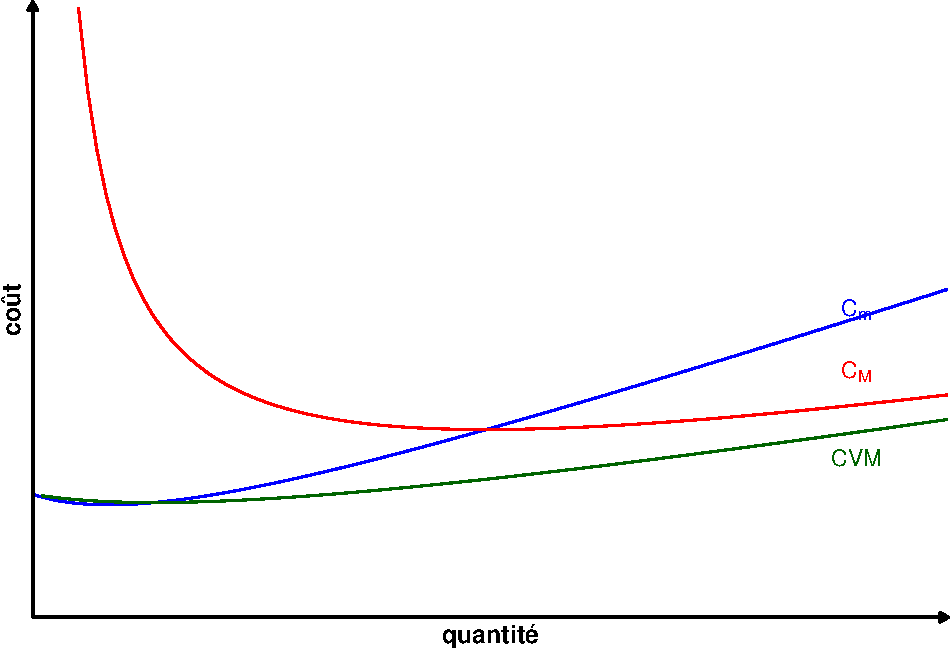
\includegraphics{_main_files/figure-latex/cppcout-1.pdf}
\caption{\label{fig:cppcout}Exemples de fonctions de coût.}
\end{figure}

\hypertarget{loffre-du-producteur}{%
\subsection{L'offre du producteur}\label{loffre-du-producteur}}

\begin{definition}[Recette totale]
La recette totale, notée \(RT\), est le produit de la vente des unités de biens.
Pour \(q\) unités de bien vendus, le producteur gagne \(RT(q)\), autrement dit, c'est le chiffre d'affaire du producteur (pour ce bien).
\end{definition}

\begin{definition}[Recette marginale]
La recette marginale, notée \(R_m\) est la recette rapportée par une unité supplémentaire de bien.
\[R_m(q)=RT'(q)\]
\end{definition}

\begin{definition}[Profit]
Le profit, noté \(\pi\) est la différence entre la recette totale est le coût total de production :
\[\pi(q)=RT(q)-CT(q)\]
\end{definition}

Le producteur choisit la quantité produite de manière à maximiser son profit.

\begin{definition}[Programme du producteur]
Le programme du producteur est :
\[\max_q\pi(q)=\max_q RT(q)-CT(q)\]
\end{definition}

\begin{theorem}[Offre du producteur]
En concurrence pure et parfaite, le programme du producteur est tel que la quantité produite \(q\) égalise coût marginal et recette marginale.
À l'optimum :
\begin{equation}
R_m(q) =c_m(q)
\label{eq:cppopti}
\end{equation}
\end{theorem}

\begin{proof}
Le programme du producteur est de maximiser son profit :
\[\max_q\pi(q)=\max_q RT(q)-CT(q)\]
À l'optimum, et à condition que les fonctions de coût et de recette soient dérivables (ce qui sera toujours le cas ici), cela signifie que l'on doit avoir la condition du premier ordre :
\[\pi'(q)=0\Leftrightarrow RT'(q)-CT'(q)=0\Leftrightarrow R_m(q)=C_m(q)\]
On obtient donc bien l'équation \eqref{eq:cppopti}
\end{proof}

L'intuition pour ce résultat est assez simple.
Si on a \(R_m(q)>C_m(q)\), alors augmenter la quantité produite rapporte plus que cela ne coûte, et donc augmente le profit.
À l'inverse, si \(R_m(q)<C_m(q)\), diminuer la quantité produite diminue plus le coût que la recette du producteur, et donc augmente le profit.
La situation s'équilibre donc pour \(R_m(q)=C_m(q)\).
Si cette égalité n'est pas vérifiée, le producteur peut en effet augmenter son profit en jouant sur la quantité produite.

En concurrence pure et parfaite, le producteur est \emph{price-taker}.
Le prix sur le marché est unique et donné , il vaut \(p\) et ne dépend pas des quantités produites par \emph{un} producteur.
Le producteur vend son bien au prix défini par le marché.
La recette totale devient donc \(RT(q)=p\times q\), avec \(p\) fixé.
La recette marginale est donc \(R_m(q)=RT'(q)=p\).
En réécrivant l'équation \eqref{eq:cppopti}, on obtient en concurrence pure et parfaite :
\[p=C_m(q)\]

\begin{proposition}[Courbe d'offre en CPP]
En concurrence pure et parfaite, la courbe d'offre du producteur est la courbe de coût marginal.
\[p=C_m(q)\]
\end{proposition}

Le profit du producteur s'écrit alors :
\[\pi(q)=RT(q)-CT(q)=pq-CT(q)=pq-C_M(q)q=q(p-C_M(q))\]
Autrement dit, le profit d'un producteur en concurrence pure et parfaite et la différence entre le prix de vente et le coût moyen de production multiplié par le nombre d'unités vendues.
Si ce prix est inférieur au coût moyen de toutes les unités vendues, le profit sera négatif.

\begin{figure}
\centering
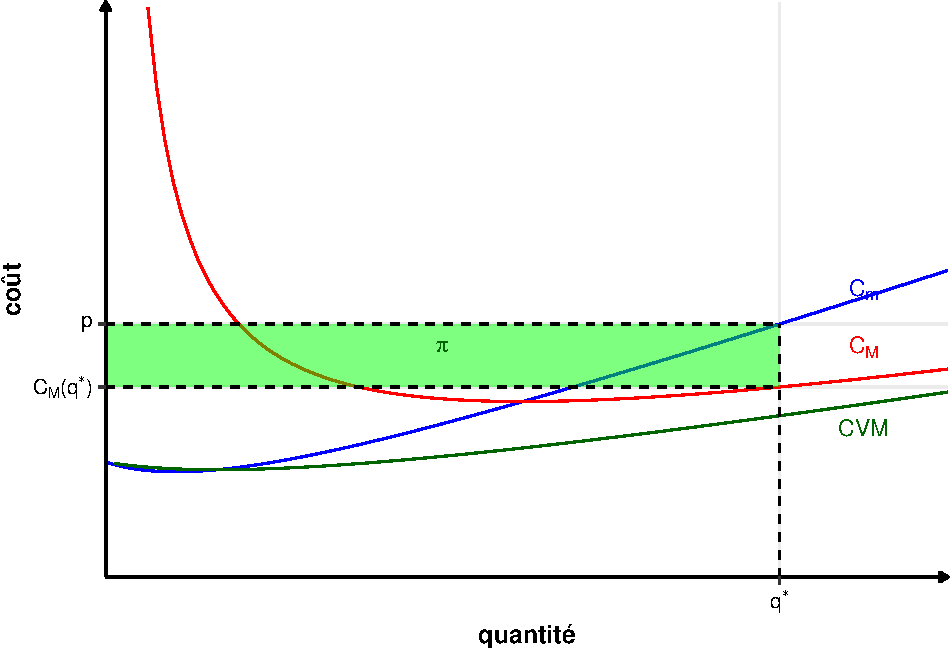
\includegraphics{_main_files/figure-latex/cppprofit-1.pdf}
\caption{\label{fig:cppprofit}Profit d'un producteur en concurrence pure et parfaite.}
\end{figure}

\hypertarget{luxe9quilibre-de-marchuxe9}{%
\section{L'équilibre de marché}\label{luxe9quilibre-de-marchuxe9}}

\begin{definition}[Demande agrégée (D)]
La \emph{demande agrégée (D)} est la somme des demandes individuelles pour chaque niveau de prix.
\end{definition}

\begin{definition}[Offre agrégée (S)]
L'\emph{offre agrégée (S)} est la somme des offres individuelles pour chaque niveau de prix.
\end{definition}

L'équilibre de marché se fait à l'intersection entre S et D (quand S=D).

\begin{figure}
\centering
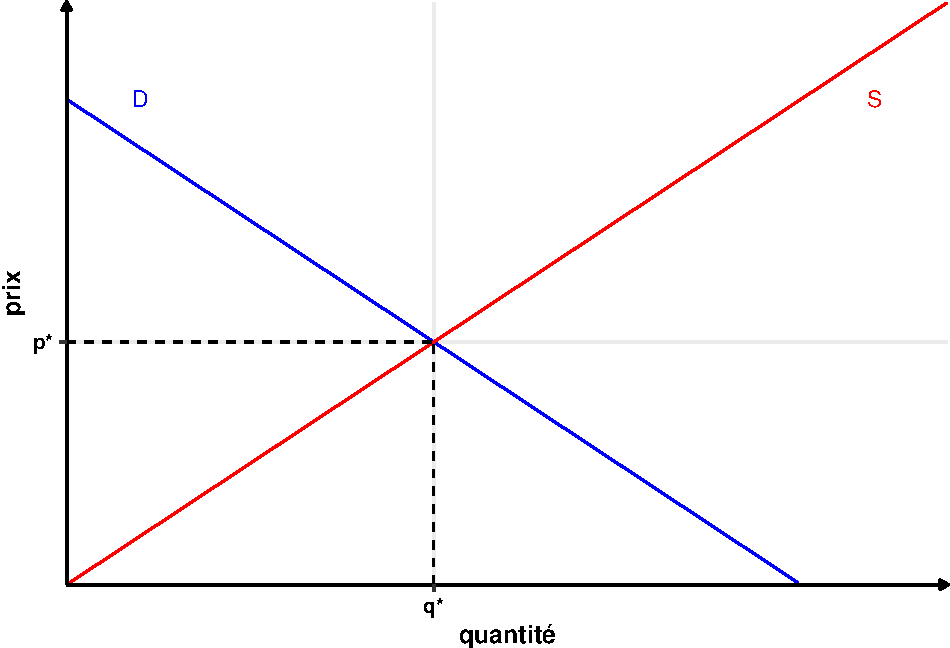
\includegraphics{_main_files/figure-latex/marche-1.pdf}
\caption{\label{fig:marche}Equilibre de marché.}
\end{figure}

La courbe de demande correspond à la suite des prix de réserve des individus, c'est-à-dire aux prix maximal que chaque individu est prêt à payer pour obtenir une unité \emph{supplémentaire} du bien.

La courbe d'offre correspond à la série des coûts marginaux de production, c'est-à-dire les prix minimaux auxquels les producteurs souhaitent vendre une unité supplémentaire du bien.

La vente de toutes les unités jusqu'à la quantité d'équilibre \(q^*\) au prix \(p^*\) procure un \emph{surplus} aux agents économiques.

\begin{definition}[Surplus des consommateurs]
Le surplus des consommateurs est la somme des différences entre le prix de réserve des consommateurs et le prix payé par le consommateur pour obtenir les biens.
Sur le graphique quantité prix \((q, p)\), c'est l'aire compris entre la courbe de demande est la droite horizontale dont l'ordonnée est le prix d'échange.
Formellement :
\[S_c=\int_0^{q^*}P(q)-p^* dq\]
\end{definition}

\begin{remark}
Seule la dernière unité de bien achetée par les consommateur l'est au prix de réserve.
Il n'y a pas de gain à l'échange pour cette unité, mais pour toutes les autres, il y en a, ce qui explique pourquoi il y a un surplus à l'échange, et pourquoi celui-ci à lieu.
\end{remark}

\begin{definition}[Surplus des producteurs]
Le surplus des producteurs est la somme des différences entre le prix auquel les producteurs vendent le bien et la courbe de coût marginal, qui représente le coût d'une unité supplémentaire produite.
Sur le graphique quantité prix \((q, p)\), c'est l'aire compris entre le prix de vente et la courbe de coût marginal.
Formellement :
\[S_p=\int_0^{q^*}p^*-S(q) dq\]
\end{definition}

En pratique, on utilisera jamais la formule avec des intégrales, mais on calculera l'aire du triangle (ou trapèze) concerné.

\begin{figure}
\centering
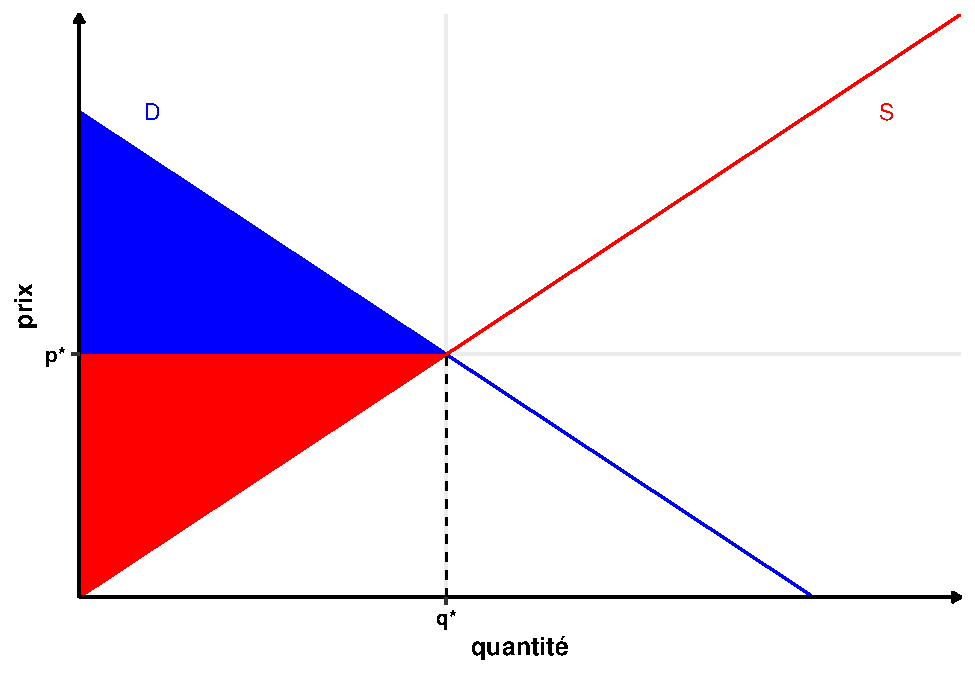
\includegraphics{_main_files/figure-latex/surplus-1.pdf}
\caption{\label{fig:surplus}Surplus des consommateurs et des producteurs.}
\end{figure}

\begin{proposition}[Propriétés de l'équilibre en concurrence pure et parfaite]
\protect\hypertarget{prp:cppprop}{}\label{prp:cppprop}L'équilibre en CPP est celui qui \textbf{maximise} le \emph{surplus total}.
Tout autre couple prix/quantité abouti à un surplus total plus faible.\\
L'équilibre de CPP est \emph{Pareto-optimal}, i.e., il est impossible d'améliorer la situation d'un agent sans détériorer celle d'un autre.
C'est ce qu'on appelle le \emph{premier théorème du bien-être}.
\end{proposition}

Ces propriétés font de la CPP une ``référence'' par rapport à laquelle on peut comparer les résultats des autres structures de marché.

\hypertarget{perception-par-les-agents-isoluxe9s}{%
\section{Perception par les agents isolés}\label{perception-par-les-agents-isoluxe9s}}

L'hypothèse d'atomicité indique que les agents individuels sont isolés au sein d'un très grand nombre d'autres agents.
Ainsi, aucun agent n'a d'influence sur le prix s'il modifie son comportement.
Une conséquence directe est que le comportement des autres agents est perçu comme étant infiniment élastique.
C'est-à-dire qu'un producteur sait qu'au prix de marché, il pourra vendre toute sa production, mais que s'il pratique un prix même légèrement plus élevé, il ne vendra \textbf{rien}.
Il perçoit ainsi une demande infiniment élastique au prix, au niveau du prix \(p^*\).

\begin{figure}

{\centering 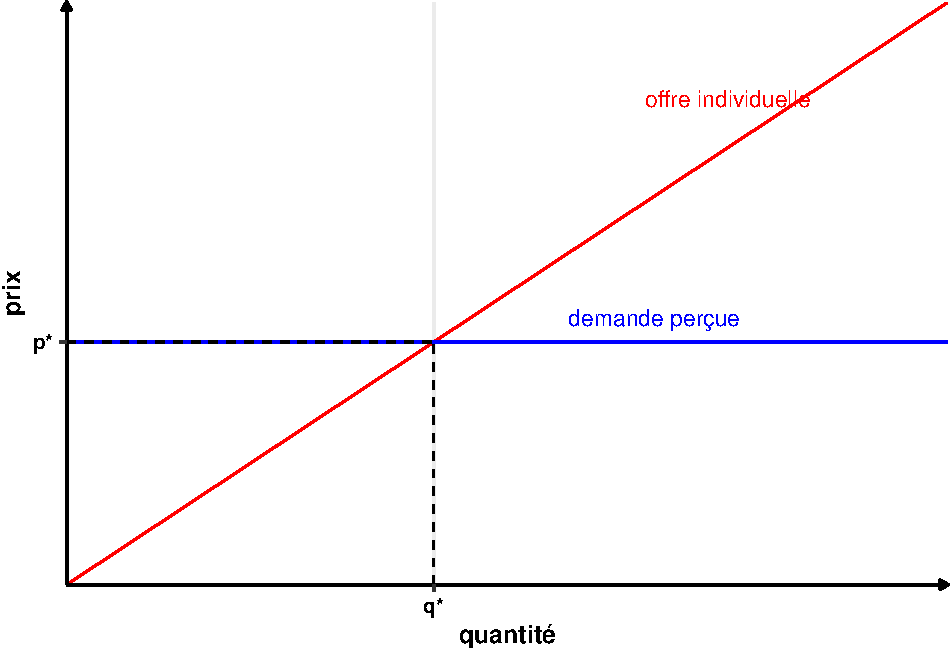
\includegraphics{_main_files/figure-latex/elasticite-1} 

}

\caption{Perception de la demande globale par un producteur isolé.}\label{fig:elasticite}
\end{figure}

Dans ce graphique, \(q^*\) représente la production optimale de ce producteur quand il est seul.

\hypertarget{le-monopole}{%
\chapter{Le monopole}\label{le-monopole}}

\begin{definition}[Monopole]
Un \emph{monopole} est sur un marché donné l'unique entreprise qui produit le bien.
\end{definition}

C'est le cas extrême opposé à la concurrence pure et parfaite, du côté du producteur.
Il est intéressant à étudier car il nous renseigne sur les principaux aspects du comportement des entreprises dans les cas intermédiaires.

Il y a de nombreuses raisons qui aboutissent à l'existence de monopoles.
Les principales sont :

\begin{itemize}
\tightlist
\item
  Légales, à cause de réglementation particulières.
  C'est ce qu'on appelle en général des professions réglementées, comme les avocats, les bureaux de tabac, les taxis\ldots{}
\item
  Légales, à cause des brevets sur une technologie données (industrie pharmaceutique\ldots) ;
\item
  Historique, le premier arrivé ;
\item
  Monopoles \emph{naturels} : en présence d'économies d'échelles, produire une quantité donnée revient moins cher avec un seul producteur qu'avec plusieurs.
  C'est notamment les cas des industries où il faut installer des réseaux (chemins de fer, électricité, téléphone, etc).
  Plus généralement, les industries avec des coûts fixes / coûts d'entrées très élevées aboutissent à des formes proches du monopole naturel (sidérurgie, automobile\ldots) ;
\item
  Exclusivité sur la production de certaines matières premières (cuivre au Chili, terres rares en Chine,\ldots) ;
\item
  Coalitions créant un cartel ;
\item
  \ldots{}
\end{itemize}

\hypertarget{recette-et-recette-marginale}{%
\section{Recette et recette marginale}\label{recette-et-recette-marginale}}

\hypertarget{duxe9finition}{%
\subsection{Définition}\label{duxe9finition}}

À la différence du cas de la concurrence pure et parfaite, le monopole perçoit la courbe de demande agrégée, et non plus celle avec une élasticité infinie.
Le choix de la quantité qu'il met sur le marché modifie le prix auquel il pourra vendre sa production, et il le sait.\\
Il va choisir \textbf{un} des paramètres du couple \((q, P(q))\), et l'autre en découlera, à travers la demande inverse \(P(q)\).
Autrement dit, s'il choisit \(q\), \(P(q)\) sera déterminé par la demande (inverse).
Si, au contraire, il choisit \(P\), \(q\) sera déterminé par la demande.

En CPP, la recette totale du producteur individuel était \(R(q) = q\cdot P(q^*)\), où \(q\) est sa production individuel, \(q^*\) la quantité d'équilibre sur le marché (résultat de la production de \emph{toutes} les entreprises présentes sur le marché) et \(P(q^*)=p^*\) est le prix d'équilibre.

En monopole, le prix dépend de la production du monopole (ou l'inverse, peu importe) :
\[
R(q) = q\cdot P(q)
\]

\hypertarget{recette-marginale-et-courbe-de-demande}{%
\subsection{Recette marginale et courbe de demande}\label{recette-marginale-et-courbe-de-demande}}

Comme la courbe de demande est décroissante (l'élasticité prix de la demande est négative \(\varepsilon_{q/p} <0\)), \(P(q)\) et \(q\) ont une relation inverse.
Autrement dit, si \(q\) augmente, alors \(p\) baisse, et réciproquement.

Cela implique que la recette totale va augmenter ou baisser suivant les propriétés de la courbe de demande.

\begin{figure}
\centering
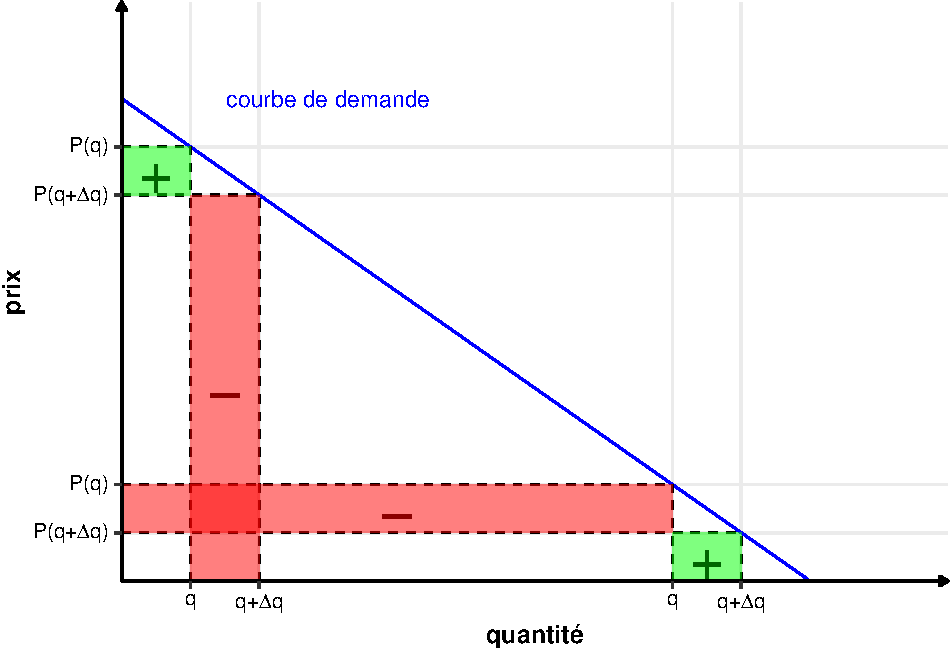
\includegraphics{_main_files/figure-latex/monorecettemarginale-1.pdf}
\caption{\label{fig:monorecettemarginale}Recette marginale d'un monopole.}
\end{figure}

Quel est le paramètre important de la courbe de demande qui détermine si le revenu \(R\) augmente ou diminue (c'est-à-dire si \(R_m\) est positive ou négative) ?

\begin{align*}
R(q) & = qP(q)\\
R_m(q)& = R'(q) \\
& = \left(qP(q)\right)' \\
& = P(q) + qP'(q) \\
& = P(q)\left(1 + \frac{q}{P(q)}P'(q) \right)\\
& = P(q)\left(1 + \frac{1}{\varepsilon_{q/p}(q)}\right)
\end{align*}

\begin{remark}[Élasticité prix de la demande]
L'élasticité prix de la demande \(\varepsilon_{q/p}\) s'écrit :
\[\varepsilon_{q/p}(p)=\frac{p}{D(p)}D'(p) <0\]
Où \(D\) est la fonction de demande.
Elle est toujours négative, car la demande diminue quand le prix augmente.
On peut la réécrire à l'aide de la fonction de demande inverse \(P\).
Comme \(D\) et \(P\) sont les fonctions réciproques l'une de l'autre, on a \(D(P(q)) = q\).
En dérivant à gauche et à droite, on obtient :
\[P'(q)D'(P(q)) = 1\]
On obtient donc :
\[P'(q)=\frac{1}{D'(p)}\]
Et l'élasticité prix de la demande peut aussi s'écrire :
\[\varepsilon_{q/p}(q)=\frac{P(q)}{q}\frac{1}{P'(q)}\]
\end{remark}

On peut donc écrire :
\begin{equation}
R_m(q) = P(q)\left(1 - \frac{1}{|\varepsilon_{q/p}(q)|}\right)
\label{eq:rm}
\end{equation}

De l'équation \eqref{eq:rm}, on observe que le signe de la recette marginale \(R_m\) dépend de l'élasticité prix de la demande.

\begin{enumerate}
\def\labelenumi{\arabic{enumi}.}
\tightlist
\item
  Si la demande est élastique (\(|\varepsilon_{q/p}(q)|>1\)), alors \(R_m(q)>0\), donc si la quantité augmente, le revenu augmente.
\item
  Si la demande est inélastique (\(|\varepsilon_{q/p}(q)|<1\)), alors \(R_m(q)<0\), donc si la quantité augmente, le revenu diminue.
\end{enumerate}

Une représentation graphique de l'allure générale est donnée dans la figure \ref{fig:monopoleelasticite}

\begin{figure}
\centering
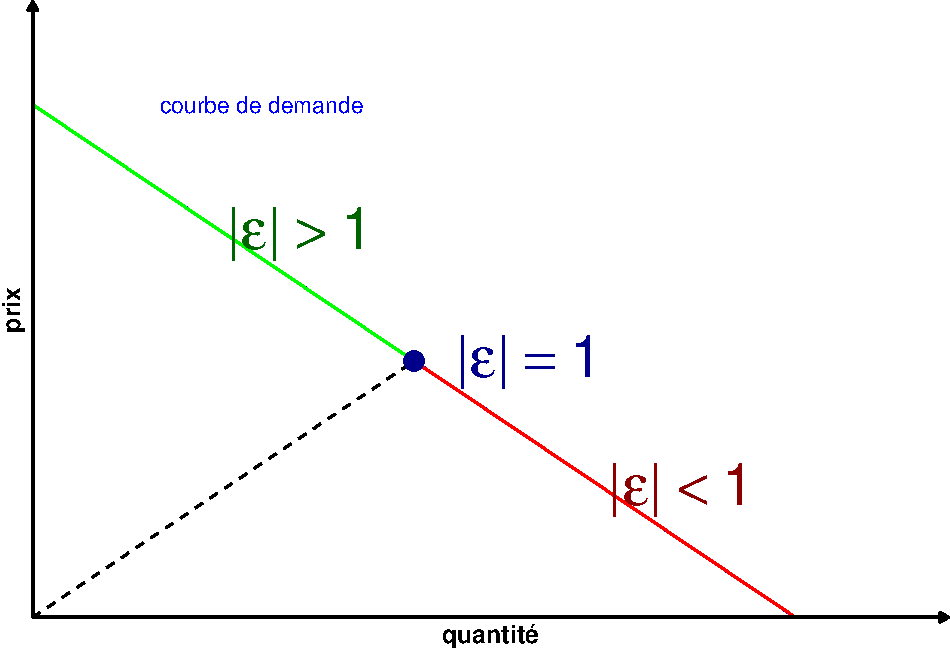
\includegraphics{_main_files/figure-latex/monopoleelasticite-1.pdf}
\caption{\label{fig:monopoleelasticite}La recette marginale est maximale lorsque l'élasticité prix de la demande est égale à -1.}
\end{figure}

\hypertarget{repruxe9sentation-graphique}{%
\subsection{Représentation graphique}\label{repruxe9sentation-graphique}}

La courbe de recette marginale est toujours située en-dessous de la courbe de demande :
\[
R_m(q) = P(q) + qP'(q) < P(q)
\]
et \(P'(q)\) est négative (la demande inverse est décroissante).

\hypertarget{exemple-avec-une-courbe-de-demande-linuxe9aire}{%
\subsubsection{Exemple avec une courbe de demande linéaire}\label{exemple-avec-une-courbe-de-demande-linuxe9aire}}

Prenons maintenant l'exemple d'une courbe de demande inverse linéaire quelconque \(P(q) = a-bq\) (\(a\) et \(b\) sont des paramètres quelconques).
On obtient alors \(R_m(q) = a-2bq\) (et \(R(q) = aq-bq^2\)).\\
Dans le cas linéaire, le revenu marginal est une droite de pente deux fois plus élevée que la demande, et ayant la même ordonnée à l'origine.
La recette marginale divise en deux tout segment horizontal entre l'axe des ordonnées et la courbe de demande inverse.
On peut ainsi représenter graphiquement, comme dans la figure \ref{fig:recettemarginale} la demande, la recette marginale et la recette totale.

\begin{figure}
\centering
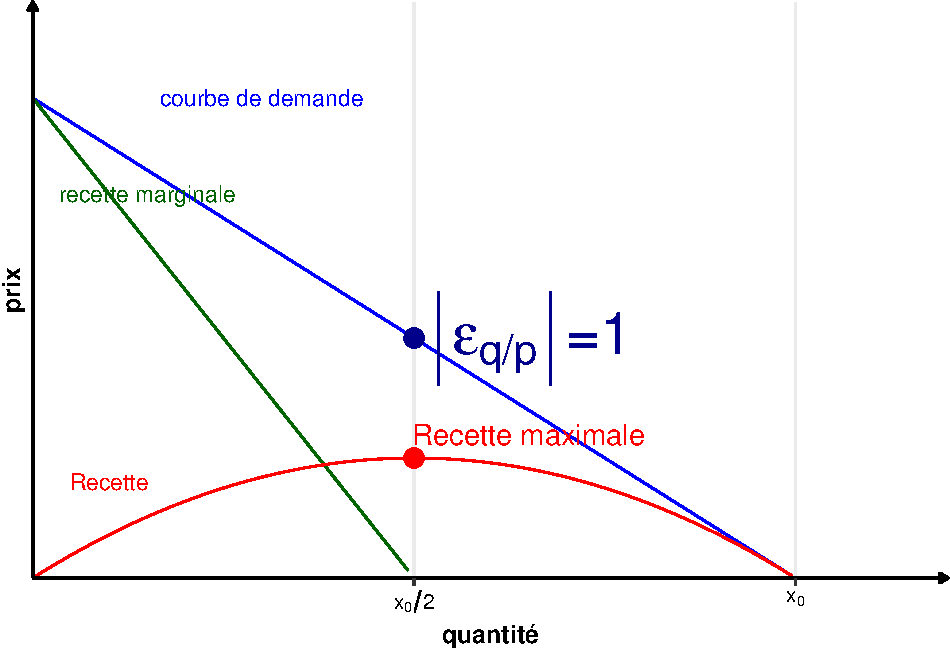
\includegraphics{_main_files/figure-latex/recettemarginale-1.pdf}
\caption{\label{fig:recettemarginale}Elasticité et recette.}
\end{figure}

La recette maximale est atteinte lorsque la valeur absolue de l'élasticité prix de la demande est égale à 1 (\(|\varepsilon_{q/p}(q)|=1\)).

\begin{figure}
\centering
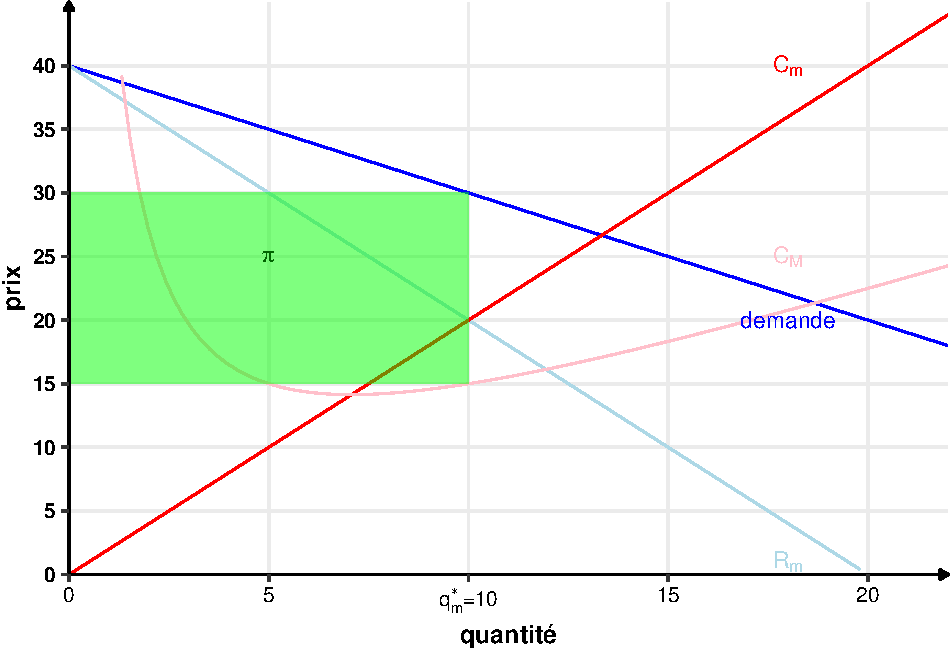
\includegraphics{_main_files/figure-latex/monopoleprofit-1.pdf}
\caption{\label{fig:monopoleprofit}Recette maximale.}
\end{figure}

Sur la figure \ref{fig:monopoleprofit}, on voit qu'il est possible de calculer la recette totale de deux manières :

\begin{enumerate}
\def\labelenumi{\arabic{enumi}.}
\tightlist
\item
  En utilisant l'aire du trapèze vert (intégrale de la recette marginale entre 0 et la quantité échangée \(q^*\)) ;
\item
  En utilisant l'aire du rectangle rouge (\(\pi=p^* q^*\)).
\end{enumerate}

Le résultat donne l'égalité d'aire entre le triangle vert et le triangle rouge.

\hypertarget{duxe9cision-de-production-du-monopole}{%
\section{Décision de production du monopole}\label{duxe9cision-de-production-du-monopole}}

\hypertarget{maximisation-du-profit}{%
\subsection{Maximisation du profit}\label{maximisation-du-profit}}

Comme dans le cas de la CPP, on suppose que le monopole cherche à maximiser son profit \(\pi(q)=R(q)-C(q)\), où \(C(q)\) est la fonction de coût (total) du monopole.\\
Il y a 2 conditions d'optimalités, les conditions de premier (la dérivée du profit à l'optimum est nulle: \(\pi'(q^*)=0\)) et de second ordre (la dérivée seconde du profit à l'optimum est strictement négative \(\pi''(q^*)<0\)), ainsi qu'une contrainte, que le profit à l'optimum soit positif (\(\pi(q^*)>0\)).

La condition de premier ordre s'exprime ainsi :
\[
\begin{array}{rcl}
\pi'(q^*) &=&0\\
\Leftrightarrow R'(q^*) - C'(q^*) &=& 0\\
\Leftrightarrow R_m(q^*) &=&C_m(q^*) 
\end{array}
\]
À l'optimum, le monopole égalise le coût marginal et le revenu marginal.

La condition du second ordre s'exprime ainsi :
\[
\begin{array}{rcl}
\pi''(q^*) &<&0\\
\Leftrightarrow R_m'(q^*) - C_m'(q^*) &<& 0\\
\Leftrightarrow R_m'(q^*) &<& C_m'(q^*)
\end{array}
\]

La dérivée de la recette marginale doit être inférieure à la dérivée du coût marginal.
Autrement dit, la recette marginale doit croître moins vite que le coût marginal.
Cette condition est en particulier vérifiée si la recette marginale est décroissante et le coût marginal croissant.

Finalement, il faut vérifier que le profit à l'optimum est positif (\(\pi(q^*)>0\)).
Dans le cas contraire, le marché n'existerait tout simplement pas, car le monopole ne voudrait pas produire le bien.

\begin{theorem}[Optimum du du monopole]
À l'optimum, le monopole égalise le coût marginal et le revenu marginal.
Ce n'est un maximum que si la dérivée de la recette marginale est inférieure à la dérivée du coût marginal et que le profit est positif.
\begin{equation}
R_m(q^*)=C_m(q^*) 
\label{eq:cpo}
\end{equation}
\begin{equation}
R_m'(q^*) <C_m'(q^*) \label{eq:cso}
\end{equation}
\begin{equation}
\pi(q^*)>0 \label{eq:profitpos}
\end{equation}
\end{theorem}

On peut comprendre graphiquement pourquoi il faut que le coût marginal et la recette marginale soient égaux (figure \ref{fig:monopoleoptimale}).
Si le monopole produit plus que \(q_m^*\), alors chaque unité produite en plus lui coûte plus chère qu'elle ne lui rapporte.
A l'inverse, s'il produit moins, produire des unités en plus lui rapporterait plus que cela ne lui coûte.

\begin{figure}
\centering
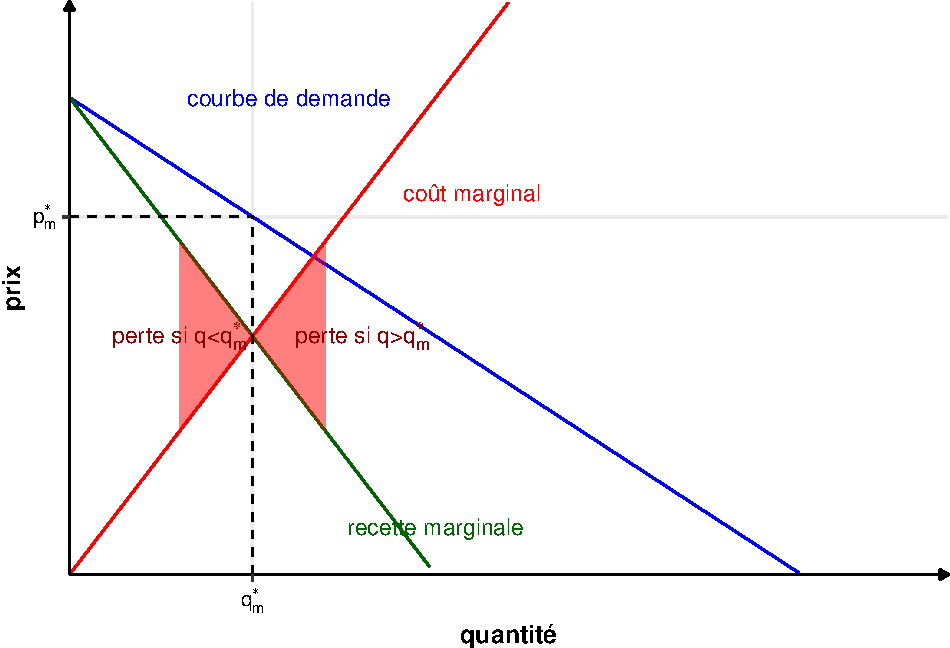
\includegraphics{_main_files/figure-latex/monopoleoptimale-1.pdf}
\caption{\label{fig:monopoleoptimale}Production optimale du monopole.}
\end{figure}

Le prix est lu et obtenu sur la courbe de \textbf{demande}.

\begin{example}[Maximisation du monopole]
\protect\hypertarget{exm:monopoleexemple}{}\label{exm:monopoleexemple}Prenons un monopole avec une fonction de coût \(C(q)=50+q^2\).
Le monopole fait face à une demande inverse \(P(q) = 40-q\).

Le coût marginal est :
\[
C_m(q) = C'(q)=2q
\]

La recette totale est :
\[
R(q) = qP(q) = q(40-q) = 40q-q^2
\]
La recette marginale est donc :
\[
R_m(q) = R'(q) = 40 - 2q
\]
Le profit vaut :
\[
\pi(q) = R(q)-C(q)
\]
Conformément à l'équation \eqref{eq:cpo}, il est maximal lorsque :
\[
\begin{array}{rcl}
R_m(q^*) &=&C_m(q^*)\\
\Leftrightarrow 40 -2q &= &2q\\
\Leftrightarrow q^*&=&10
\end{array}
\]
La condition de second ordre de l'équation \eqref{eq:cso} est bien vérifiée, car \(-2<2\).

Le prix de vente vaut :
\[P(q^*) = P(10) = 40-10 = 30\]
La recette vaut 300, le coût 150.
On a donc un profit de \textbf{150}, qui est bien positif (condition de l'équation \eqref{eq:profitpos}.
\end{example}

\begin{figure}
\centering
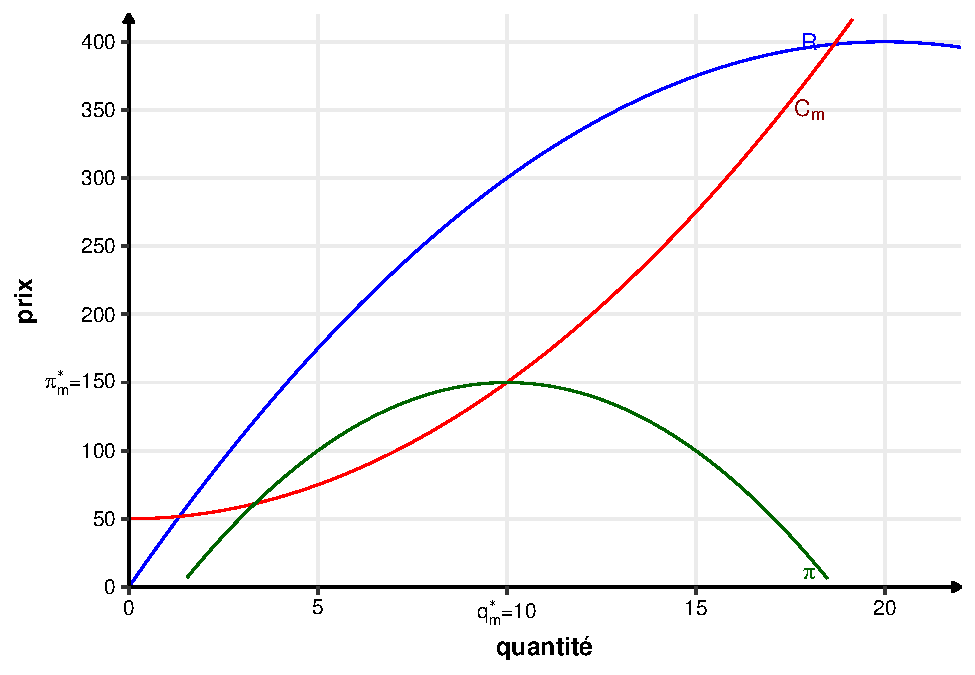
\includegraphics{_main_files/figure-latex/monopolerecette-1.pdf}
\caption{\label{fig:monopolerecette}Recette, coût et profit dans l'exemple \ref{exm:monopoleexemple}.}
\end{figure}

\begin{figure}
\centering
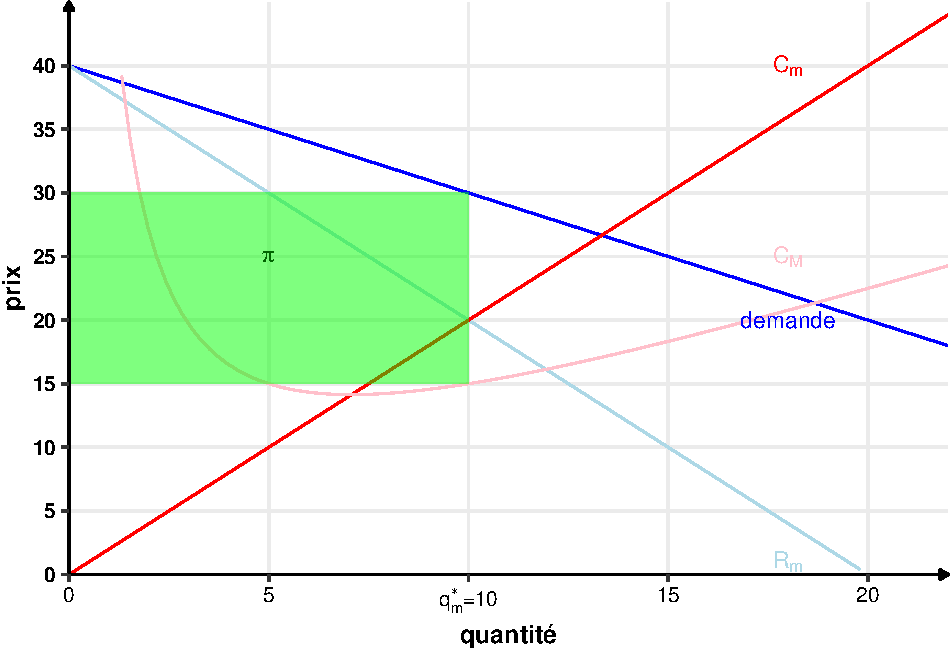
\includegraphics{_main_files/figure-latex/monopoleprofitexemple-1.pdf}
\caption{\label{fig:monopoleprofitexemple}Demande, prix, coûts et profits dans l'exemple \ref{exm:monopoleexemple}.}
\end{figure}

\hypertarget{propriuxe9tuxe9s-de-la-solution-de-la-maximisation-du-monopole}{%
\subsection{Propriétés de la solution de la maximisation du monopole}\label{propriuxe9tuxe9s-de-la-solution-de-la-maximisation-du-monopole}}

On avait dans l'équation \eqref{eq:rm} :
\[
R_m(q) = P(q)\left(1 - \frac{1}{|\varepsilon_{q/p}(q)|}\right)
\]
Comme à l'optimum, d'après l'équation \eqref{eq:cpo}, on doit avoir \(R_m(q^*)=C_m(q^*)\), on a :
\[
R_m(q^*) = P(q^*)\left(1 - \frac{1}{|\varepsilon_{q/p}(q^*)|}\right) = C_m(q^*) 
\label{eq:rmcm}
\]
On observe ici un lien avec la solution en CPP.
En effet, en CPP, l'élasticité de la demande au prix est perçue comme infinie, on aura donc bien \(P(q^*) = C_m(q^*)\), la solution obtenue en CPP.
Dès lors que l'élasticité de la demande au prix n'est plus infinie en revanche, on obtient :
\[
 P(q^*)=\frac{C_m(q^*)}{1 - \frac{1}{\left|\varepsilon_{q/p}(q^*)\right|}} > C_m(q^*)
\]

\emph{Question :} Dans quelle zone d'élasticité le monopole va-t-il opérer ?

On voit que si \(\left|\varepsilon_{q/p}(q^*)\right|<1\), c'est-à-dire que si la demande est inélastique, alors \(1 - \frac{1}{\left|\varepsilon_{q/p}(q^*)\right|} <0\), ce qui implique que la recette marginale \(R_m\) est négative, et donc impossible à égaliser avec le coût marginal \(C_m\).\\
On peut voir la réponse d'une autre façon.
Si la pente est inélastique, alors le revenu \(R\) augmente quand la quantité \(q\) baisse.
Le coût total \(C\) baisse aussi quand la quantité baisse.
Le monopole aurait donc tout intérêt à réduire sa production lorsque la demande est inélastique.

\begin{corollary}
Le monopole opère donc nécessairement dans la zone élastique de la courbe de demande : \(\left|\varepsilon_{q/p}(q^*)\right|>1\) .
\end{corollary}

\hypertarget{indice-de-pouvoir-du-monopole}{%
\subsection{Indice de pouvoir du monopole}\label{indice-de-pouvoir-du-monopole}}

La capacité du monopole à vendre à un prix supérieur au coût marginal dépend de la plus ou moins grande élasticité de la demande au prix.
Cela permet de construire un indice du \emph{pouvoir de monopole} à partir de l'élasticité du prix à la demande à l'équilibre.
On a, d'après l'équation \eqref{eq:rmcm} :
\[
R_m(q^*) = P(q^*)\left(1 - \frac{1}{|\varepsilon_{q/p}(q^*)|}\right) = C_m(q^*) 
\]
On en déduit :

\[\begin{array}{rl}
& C_m(q^*) = P(q^*) - \frac{P(q^*)}{|\varepsilon_{q/p}(q^*)|}\\
\Leftrightarrow & P(q^*) - C_m(q^*) = \frac{P(q^*)}{|\varepsilon_{q/p}(q^*)|}
\end{array}
\]

\begin{definition}[Indice de Lerner]
\protect\hypertarget{def:Lerner}{}\label{def:Lerner}On définit l'indice de Lerner \(L\) par :
\[
L=\frac{1}{|\varepsilon_{q/p}(q^*)|} = \frac{P(q^*) - C_m(q^*)}{P(q^*)} \label{eq:Lerner}
\]
L'indice de Lerner est donc inversement proportionnel à l'élasticité prix de la demande.
Il est aussi égal à la capacité du monopole à vendre au-dessus de son coût marginal, en pourcentage du prix total.
\end{definition}

On peut construire à partir de l'équation précédente le \emph{markup pricing}.

\begin{definition}[Markup pricing]
\[
P(q^*) =\frac{|\varepsilon_{q/p}(q^*)|}{|\varepsilon_{q/p}(q^*)|-1} C_m(q^*)
\]
\end{definition}

\hypertarget{variation-de-la-demande}{%
\subsection{Variation de la demande}\label{variation-de-la-demande}}

Les décisions de production du monopole et la fixation de son prix dépendent de la demande à laquelle il fait face et du coût marginal.
Le monopole n'a \textbf{pas de courbe d'offre} au sens où il n'y a pas de relation univoque entre prix et quantité produite, à la différence des producteurs en CPP.
En monopole, si la demande change, le monopole s'adapte, soit en changeant sa production, mais pas son prix (figure \ref{fig:monopolechangementdemande2}), ou l'inverse (figure\ref{fig:monopolechangementdemande1}).

\begin{figure}
\centering
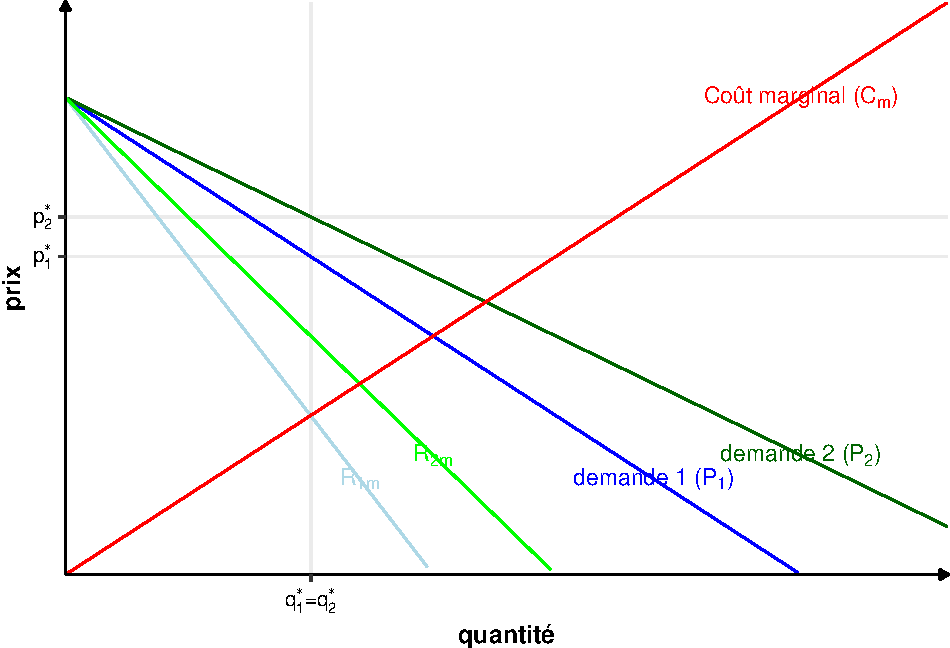
\includegraphics{_main_files/figure-latex/monopolechangementdemande1-1.pdf}
\caption{\label{fig:monopolechangementdemande1}Exemple de réaction du monopole à un changement de demande: changement de prix.}
\end{figure}

\begin{figure}
\centering
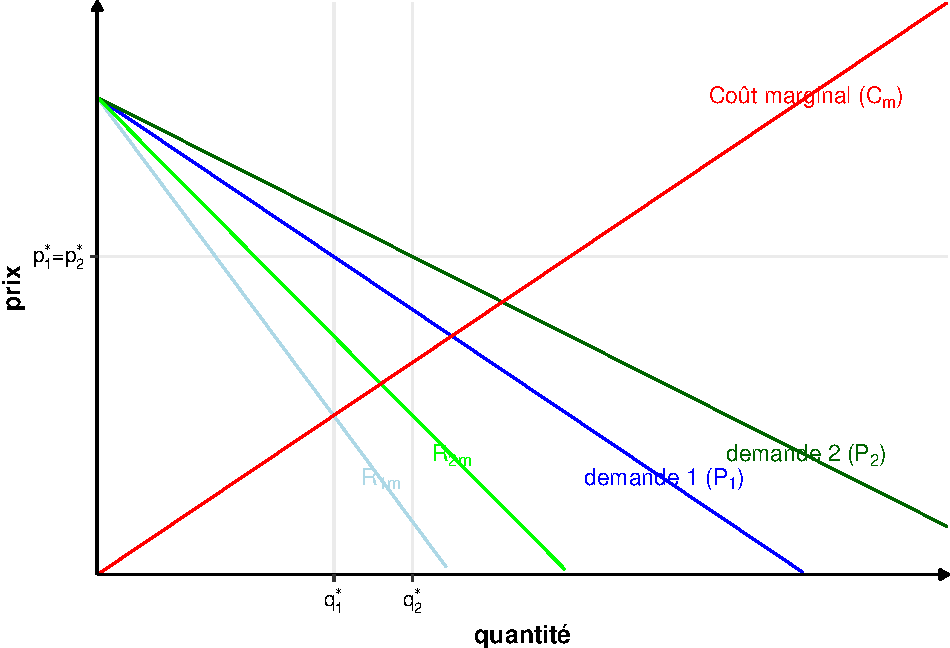
\includegraphics{_main_files/figure-latex/monopolechangementdemande2-1.pdf}
\caption{\label{fig:monopolechangementdemande2}Exemple de réaction du monopole à un changement de demande: changement de quantité.}
\end{figure}

En CPP, un changement de demande, si elle implique une changement du prix d'équilibre, entraîne forcément un changement dans la quantité produite par un producteur individuel.

\hypertarget{linefficience-du-monopole}{%
\subsection{L'inefficience du monopole}\label{linefficience-du-monopole}}

La production du monopole est inférieure à la production en CPP et le prix est supérieur au prix de CPP.

\begin{figure}
\centering
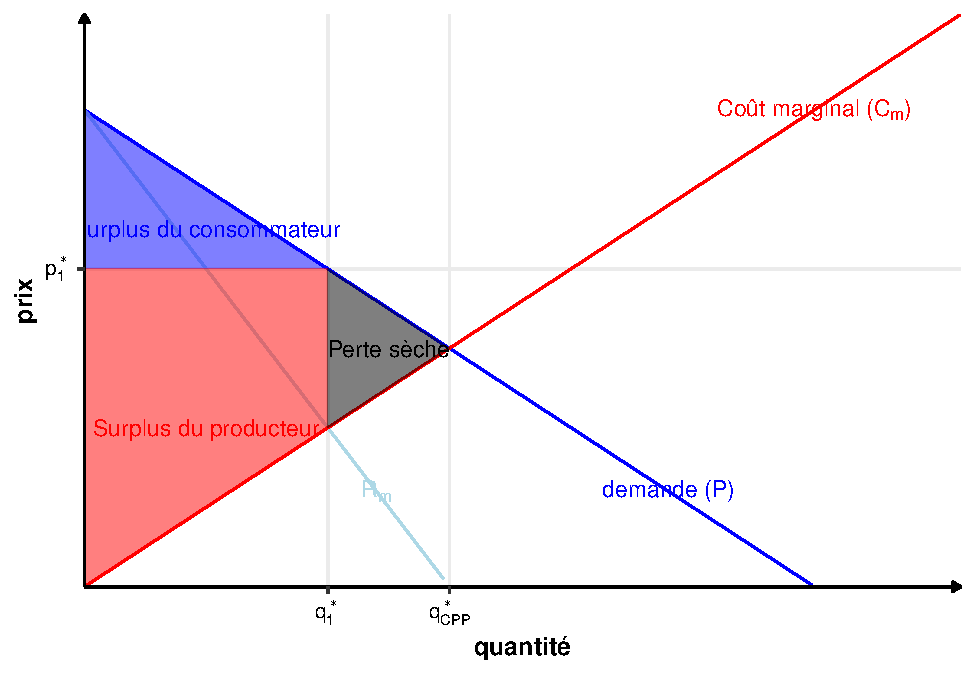
\includegraphics{_main_files/figure-latex/monosurplus-1.pdf}
\caption{\label{fig:monosurplus}Surplus quand le producteur est en monopole.}
\end{figure}

Cela signifie que le surplus du producteur (son profit) est plus élevé en monopole qu'en CPP, et que le surplus des consommateur est plus faible.
Il y a globalement une perte sèche de surplus total.
\textbf{Le monopole est inefficace au sens de Pareto.}
Il existe des consommateurs prêt à acheter à un prix supérieur au coût marginal (dans le triangle de la perte sèche).
Il est donc possible d'avoir une amélioration parétienne qui améliore à la fois la situation des consommateurs et du monopole.
Il suffirait pour cela que le monopole produise une unité supplémentaire du bien à un prix supérieur au coût marginal, sans rien changer d'autre pour obtenir cette amélioration.

\hypertarget{ruxe9gulation-du-monopole}{%
\section{Régulation du monopole}\label{ruxe9gulation-du-monopole}}

Cette partie va traiter de la manière dont un gouvernement peut inciter un monopole à modifier son comportement.

\hypertarget{taxe-unitaire}{%
\subsection{Taxe unitaire}\label{taxe-unitaire}}

Un gouvernement impose une taxe de \(t\) unités monétaire par unité de bien produite.
On a donc :

\[
\pi(q) = R(q) - C(q) -tq
\]
La condition de première ordre de la maximisation du producteur de l'équation \eqref{eq:cpo} devient alors :
\[
\begin{array}{rl}
&(R(q)-C(q) -tq)'(q^*) = 0\\
\Leftrightarrow & R_m(q^*)-C_m(q*) -t = 0\\
\Leftrightarrow & R_m(q^*) = C_m(q^*) + t
\end{array}
\]
Le problème est exactement le même que précédemment, en intégrant la taxe dans le coût marginal.
Pour le monopole, c'est comme si l'état ajoutait un coût \(t\) à chaque unité produite, ce qui est effectivement ce que l'État fait.

\begin{figure}
\centering
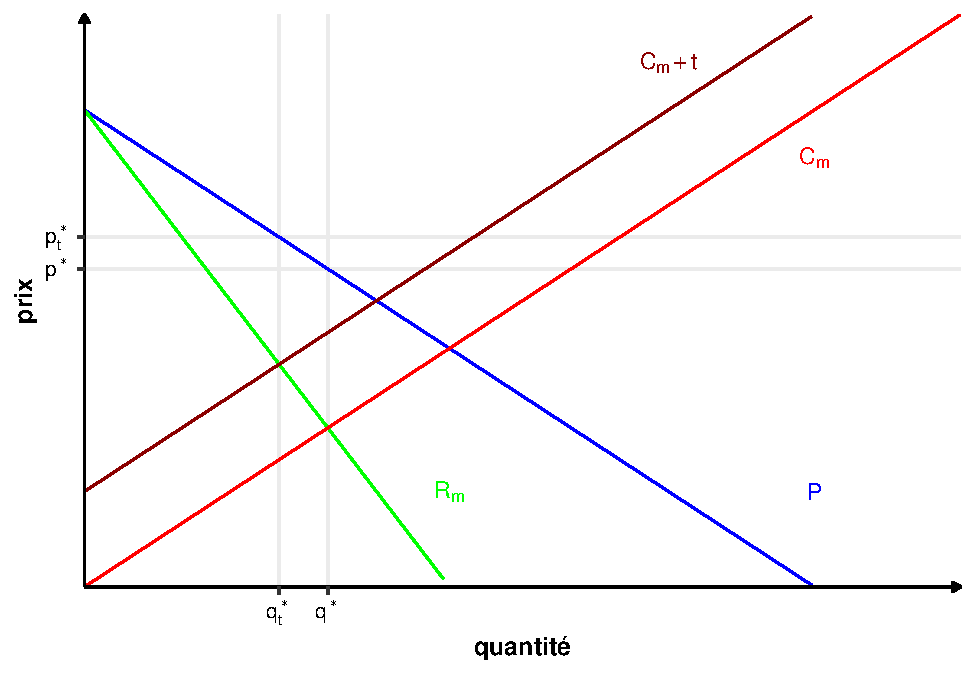
\includegraphics{_main_files/figure-latex/monopoletaxeunitaire-1.pdf}
\caption{\label{fig:monopoletaxeunitaire}Impact d'une taxe unitaire : augmentation du coût marginal.}
\end{figure}

Cela entraîne une diminution de la quantité produite et une augmentation du prix.
Le surplus des consommateurs baisse, ainsi que celui du monopole.

Une vue \textbf{alternative} à l'augmentation du coût marginal est de considérer que la taxe diminue la recette marginale de \(t\) :
\[
 R_m(q^*) -t = C_m(q^*)
\]

\begin{figure}
\centering
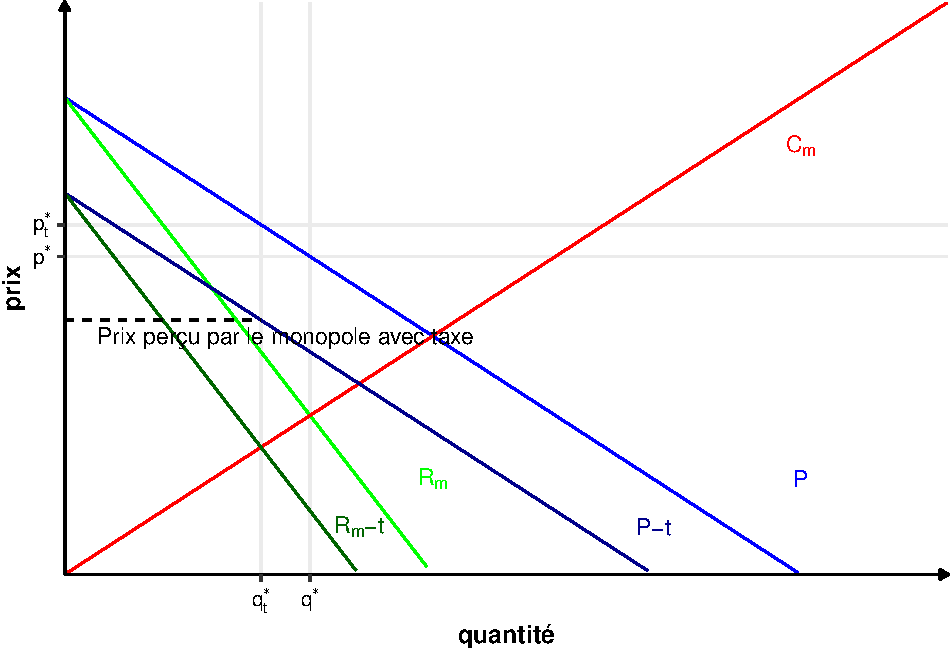
\includegraphics{_main_files/figure-latex/monopoletaxeunitaire2-1.pdf}
\caption{\label{fig:monopoletaxeunitaire2}Impact d'une taxe unitaire : diminution de recette marginale.}
\end{figure}

Si le gouvernement utilise une taxe négative (= une subvention), alors le gouvernement peut augmenter la production et de diminuer le prix.

\hypertarget{taxe-forfaitaire}{%
\subsection{Taxe forfaitaire}\label{taxe-forfaitaire}}

Avec une taxe forfaitaire, l'état prélève un montant \(T\) indépendant de la quantité produite sur le profit du producteur.
\[
\pi(q) = R(q) - C(q) -T
\]
La condition du premier ordre de l'équation \eqref{eq:cpo} devient alors :
\[
\begin{array}{rl}
& (R(q)-C(q) -T)'(q^*) = 0\\
\Leftrightarrow & R_m(q^*)-C_m(q*) = 0\\
\Leftrightarrow & R_m(q^*) = C_m(q^*)
\end{array}
\]
On retrouve exactement la même condition d'optimalité qu'en l'absence de taxe.
Si elle n'est pas trop élevée, une taxe forfaitaire n'a \emph{aucune} influence sur la quantité produite et prix.
Si la taxe forfaitaire est très élevée, supérieure au profit \(R(q^*) - C(q^*) <T\), le monopole préfère ne rien produire et le surplus social est nul.

On peut donc envisager de combiner une subvention unitaire au monopole combinée à une taxe forfaitaire pour augmenter le surplus total.

\hypertarget{impuxf4t-sur-profit}{%
\subsection{Impôt sur profit}\label{impuxf4t-sur-profit}}

Au lieu de taxer chaque unité produite, on peut taxe le niveau de profit à un taux \(t\).
Le profit devient alors
\[
\pi(q) = R(q) - C(q) -t( R(q) - C(q)) = (1-t)(R(q) - C(q))
\]
La condition du premier ordre de l'équation \eqref{eq:cpo} devient alors :
\[
\begin{array}{rl}
&((1-t)(R(q)-C(q)))'(q^*) = 0\\
\Leftrightarrow & (1-t)(R_m(q^*)-C_m(q*)) = 0\\
\Leftrightarrow & R_m(q^*) = C_m(q^*)
\end{array}
\]

Comme pour la taxe forfaitaire, le comportement du monopole n'est pas modifié par une taxe sur le profit.
On peut donc aussi envisager une subvention à la production et une taxe proportionnelle sur le profit.

\hypertarget{fixation-dun-prix-maximum}{%
\subsection{Fixation d'un prix maximum}\label{fixation-dun-prix-maximum}}

Le gouvernement interdit de vendre au-dessus d'une prix maximum \(p^{max}\)

Le gouvernement modifie ainsi la demande perçue par le producteur.

\begin{figure}
\centering
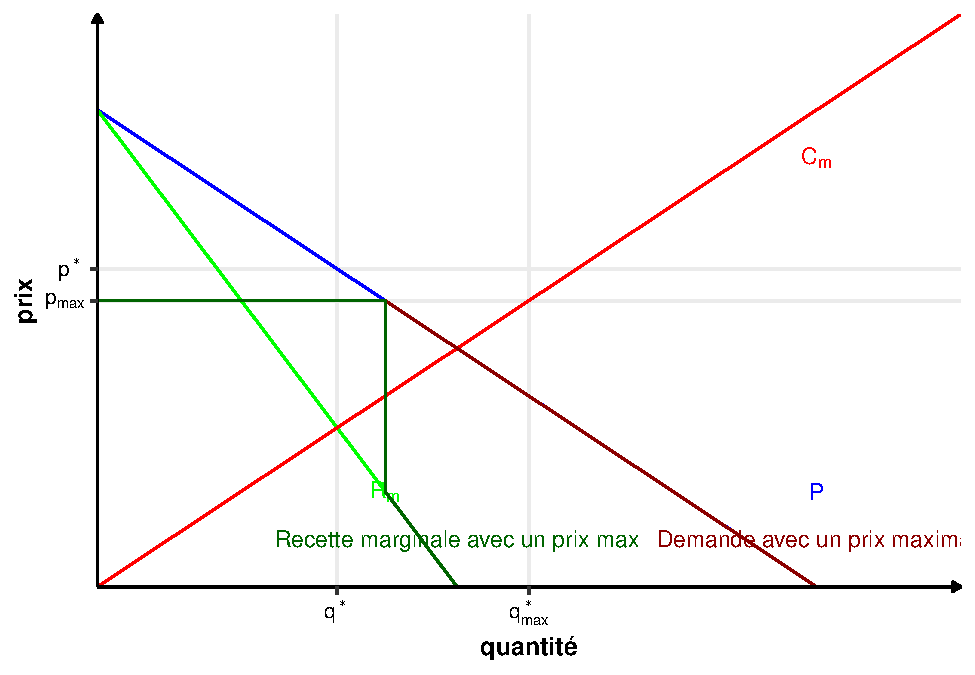
\includegraphics{_main_files/figure-latex/monopoleprixmaximal-1.pdf}
\caption{\label{fig:monopoleprixmaximal}Fixation d'un prix maximal supérieur au prix de CPP.}
\end{figure}

\begin{figure}
\centering
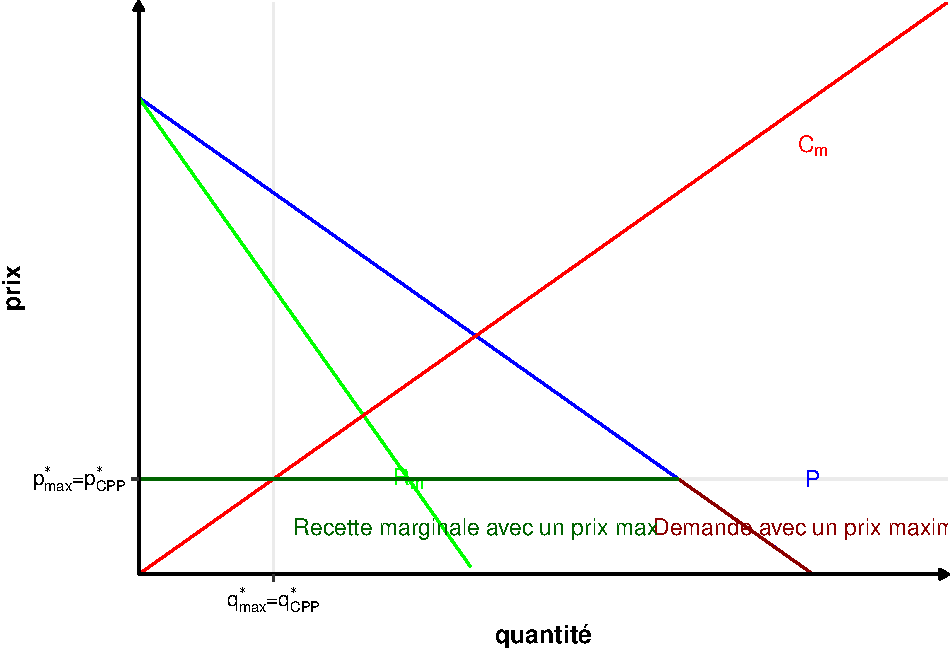
\includegraphics{_main_files/figure-latex/monopoleprixmaximal2-1.pdf}
\caption{\label{fig:monopoleprixmaximal2}Fixation d'un prix maximal inférieur au prix de CPP.}
\end{figure}

Si le prix maximum est inférieur au prix de concurrence pure et parfaite, les quantités produites peuvent devenir sous-optimale.
Le gouvernement peux maximiser le surplus social en prenant le prix concurrentiel comme prix maximum.\\
\emph{Rappel :} En CPP, on obtient le prix à l'aide de la courbe de coût marginal.
L'équilibre a lieu quand le coût marginal et la demande se croisent.

\begin{figure}
\centering
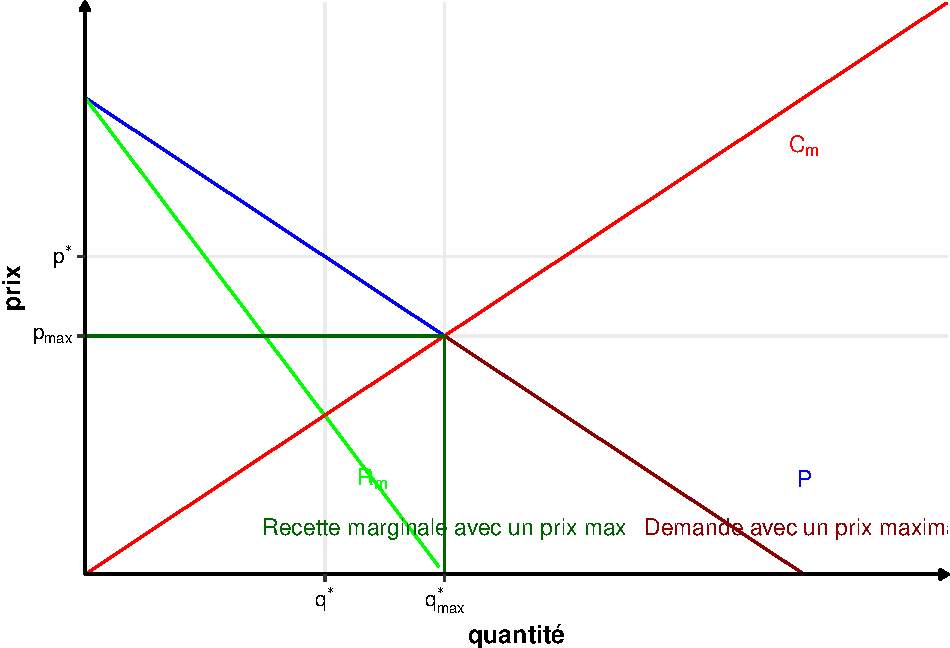
\includegraphics{_main_files/figure-latex/monopoleprixmaximalCPP-1.pdf}
\caption{\label{fig:monopoleprixmaximalCPP}Fixation d'un prix maximal égal au prix de CPP.}
\end{figure}

Avec un prix maximum égal au prix de concurrence pure et parfaite, le revenu marginal coupe la courbe de coût marginal au point d'équilibre de la concurrence pure et parfaite.

Globalement, si le prix maximal est entre le prix de monopole et le prix de concurrence pure et parfaite, alors la quantité produite augmente quand le prix maximal diminue.
Si au contraire le prix maximal est inférieur au prix de CPP (et donc de monopole), alors la quantité produite diminue quand le prix maximal augmente.

\hypertarget{le-monopole-naturel}{%
\section{Le monopole naturel}\label{le-monopole-naturel}}

Une situation de monopole naturel émerge à cause d'une structure particulière de la technologie de production et des coûts, plutôt qu'à cause d'une disposition légale.

\begin{definition}[Monopole naturel]
Un monopole naturel émerge en présence d'une technologie dotée de rendements d'échelles \emph{croissants} dans la zone de production optimale.
\end{definition}

Les rendements d'échelles sont croissants lorsque la technologie de production \(f\) est telle que :
\[
f(\lambda z_1, \lambda z_2, ...\lambda z_n) > \lambda f(z_1,z_2, ..., z_n)
\]
où les \(z_i\) sont les facteurs de productions.
En mots : une entreprise utilisant \(\lambda\) fois plus de facteurs de productions qu'une petite entreprise produit plus que \(\lambda\) petites entreprises réunies.

En général, un monopole naturel émerge à cause de coûts fixes élevés.
Par exemple, lorsqu'il faut investir dans un réseau (ferrés, téléphone, électricité, etc).

Une conséquence des rendements d'échelle croissants est que le coût moyen est décroissant :
\[
C_M(f(\lambda z)) =\frac{\lambda z\cdot w_z}{f(\lambda z)} < C_M(\lambda f(z)) = \frac{\lambda z\cdot w_z}{\lambda f(z)}
\]
car \(f(\lambda z)>\lambda f(z)\)
Cela signifie qu'une seule entreprise qui produit \(f(\lambda z)\) est plus efficace que \(\lambda\) entreprises qui produisent \(\lambda f(z)\).
Il y a ici des économies d'échelle.

\begin{definition}[Économie d'échelle]
Il y a des \emph{économies d'échelle} quand une unité de bien produite en plus revient moins chère que l'unité précédente.
Cela signifie que le \emph{coût moyen} baisse quand le producteur produit plus d'unités.
\end{definition}

De manière générale, il y a presque toujours une zone où le coût moyen est décroissant, mais elle est rarement très étendue.
Dans le graphique \ref{fig:monopolenaturelcout}, la demande inverse 1 coupe la courbe de coût marginal à un endroit où les économies d'échelle sont décroissantes.
La demande 2, en revanche, la coupe à un endroit où les économies d'échelle sont croissantes.

\begin{figure}
\centering
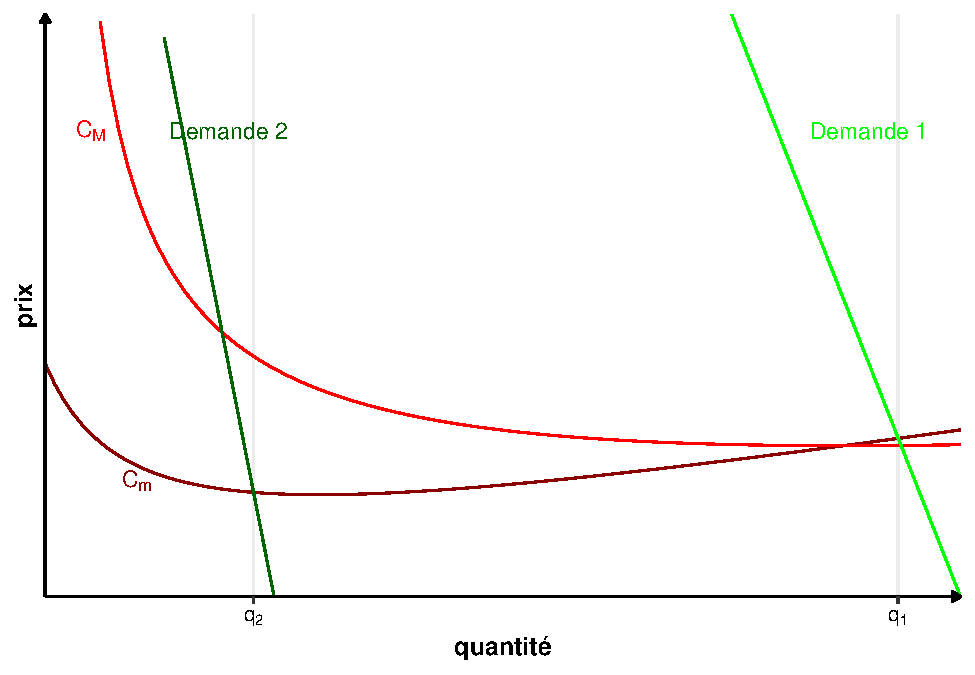
\includegraphics{_main_files/figure-latex/monopolenaturelcout-1.pdf}
\caption{\label{fig:monopolenaturelcout}Fonction de coût et demande avec et sans économies d'échelle.}
\end{figure}

\begin{remark}[Lien entre coût marginal et coût moyen en monopole naturel.]
Lorsque le coût moyen est décroissant, c'est que le coût marginal est inférieur au coût moyen.
\[
C_M(q) = \frac{C(q)}{q}
\]
\[
C_M'(q) =\frac{C'(q)q-C(q)}{q^2} = \frac{C_m(q)-C_M(q)}{q}
\]
Or \(C_M'(q)<0\), comme le coût marginal est décroissant.
On en déduit donc que
\[
C_m(q)-C_M(q)< 0 \Leftrightarrow C_m(q)<C_M(q)
\]
\end{remark}

\begin{remark}[Rendements d'échelle et économies d'échelle]
Il ne faut pas confondre les rendements d'échelle, qui mettent en relation les \textbf{quantités} de facteurs de productions et les quantités de biens produites et économies d'échelle, qui est une notion lié au \textbf{coût} de production des unités de biens produites.
\end{remark}

\textbf{Question :} Que se passe-t-il quand la fonction de demande inverse coupe la courbe de coût marginal dans la partie où le coût marginal est inférieur au coût moyen (où \(C_m<C_M\)) ?

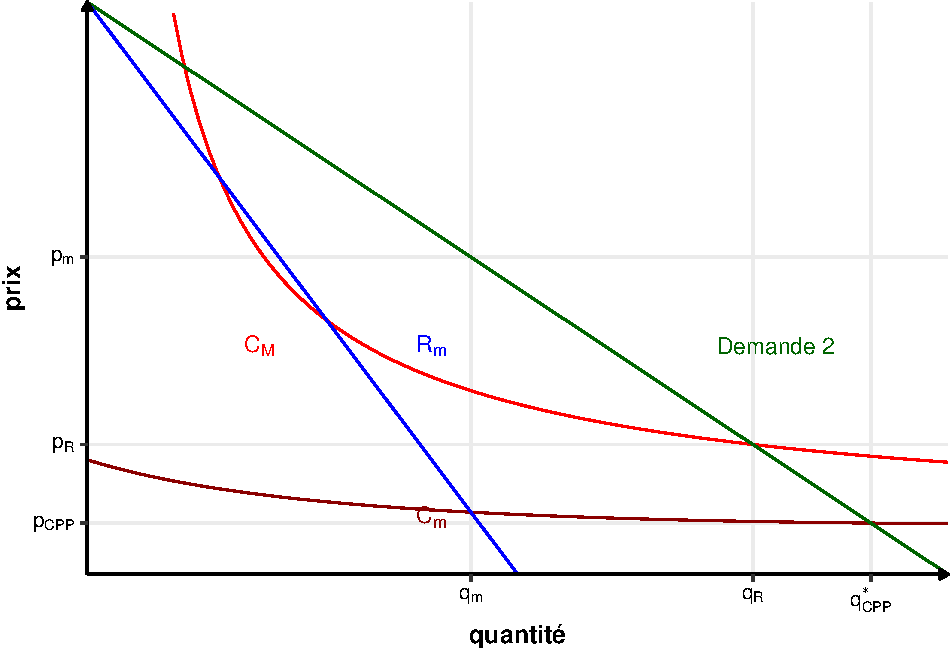
\includegraphics{_main_files/figure-latex/monopolenaturel-1.pdf}
Si on impose une tarification au coût marginal, alors le monopole fait des pertes, car le prix est inférieur au coût moyen.
La régulation ``optimale'' généralement utilisée impose \emph{un prix au coût moyen} et une obligation de satisfaire toute la demande.
Le monopole fait alors un profit nul.

Une solution alternative est un prix égal au coût moyen assorti de subventions pour couvrir les pertes.

\hypertarget{le-monopole-discriminant}{%
\section{Le monopole discriminant}\label{le-monopole-discriminant}}

Un monopole discriminant pratique un prix différent pour chaque (groupe de) consommateurs.
Pour cela, il doit pouvoir identifier l'appartenance de chaque consommateur à un groupe et les marchés entre les consommateurs doivent être hermétiques.
En particulier, il ne faut pas qu'un consommateur puisse revendre son unité de bien à un autre consommateur.

Il existe 3 types de discriminations par les prix, les discrimination du premier, deuxième et troisième degrés.
On ne traitera que les discriminations du premier et troisième degrés dans ce cours.

\hypertarget{discrimination-au-premier-degruxe9-discrimination-parfaite}{%
\subsection{Discrimination au premier degré (discrimination parfaite)}\label{discrimination-au-premier-degruxe9-discrimination-parfaite}}

Dans une discrimination parfaite, le monopole connaît la valorisation (prix de réserve) de chaque individu et lui fait payer le prix maximum qu'il est prêt à payer (son prix de réserve donc).
Le consommateur ne retient alors aucun surplus, la \emph{totalité} du surplus est capturé par le producteur.

\emph{Question :} Quel va être le niveau de production du monopole ?

Comme le monopole fait payer chaque unité à la valorisation du consommateur, la première unité est vendue au prix P(1), la deuxième au prix P(2), etc.
La recette totale est donc :
\[
R(q) = \int_0^q P(x) dx
\]
Notons le coût total \(C(q)\).
Le profit est :
\[
\pi(q) = R(q) - C(q) = \int_0^q P(x) dx -C(q)
\]
La condition du premier ordre s'écrit donc :
\[
\begin{array}{rl}
&\frac{d\pi(q^*)}{dq} = 0\\
\Leftrightarrow & \frac{d\int_0^{q^*} P(x) dx -C(q^*)}{dq} = 0\\
\Leftrightarrow & P(q^*) - C_m(q^*) = 0\\
\Leftrightarrow & P(q^*) = C_m(q^*)
\end{array}
\]
La recette marginale est ici confondue avec la courbe de demande.
L'optimum se trouve donc au point où la courbe de coût marginal coupe la courbe de demande (inverse).
C'est la même condition qu'en CPP.
Le monopole parfaitement discriminant produit donc la quantité de concurrence pure et parfaite.
Le prix de la dernière unité vendue par le monopole est égal au prix de la concurrence pure et parfaite, même si les prix des autres unités vendues sont supérieurs au prix de la CPP.

\begin{figure}
\centering
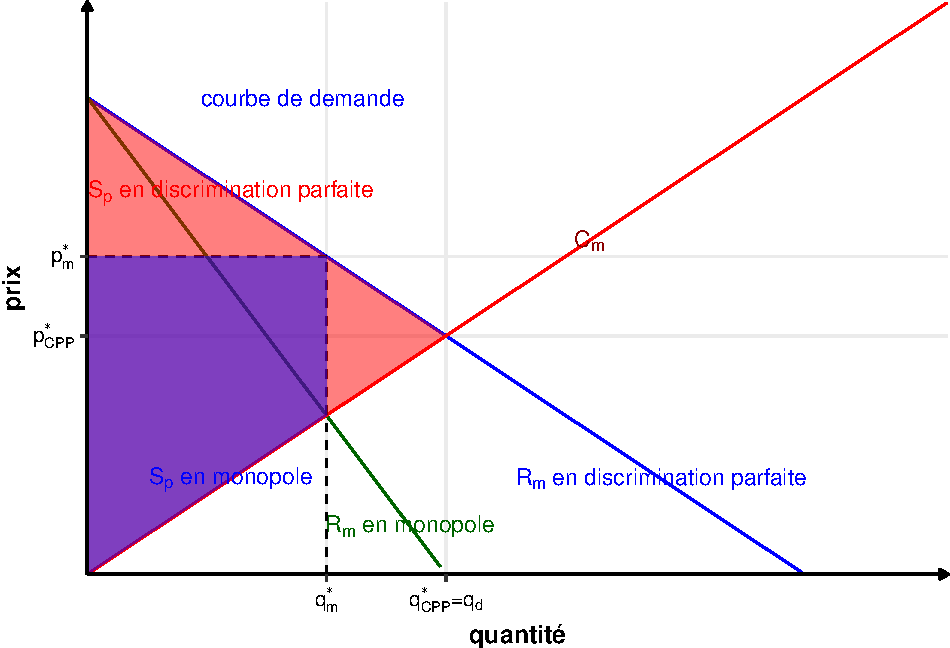
\includegraphics{_main_files/figure-latex/monopolediscriparfaite-1.pdf}
\caption{\label{fig:monopolediscriparfaite}Surplus du monopole en discrimination parfaite (aire rouge et bleue).}
\end{figure}

La situation de discrimination parfaite est un optimum de Pareto.
En effet, le surplus social est maximal (mais capturé entièrement par le monopole).

En pratique, il est très difficile de faire de la discrimination parfaite.
Les entreprises essaient de s'en approcher le plus possible.

Un exemple existe, lors d'une vente de bons du trésors des Etats-Unis.
Chaque ménage intéressé soumettait une offre (prix, quantité) au gouvernement.
Le gouvernement triait les offres par ordre décroissant de prix et les satisfait jusqu'à épuisement des bons à vendre.

\hypertarget{discrimination-du-deuxiuxe8me-degruxe9}{%
\subsection{Discrimination du deuxième degré}\label{discrimination-du-deuxiuxe8me-degruxe9}}

\begin{definition}[Discrimination du deuxième degré]
La discrimination du deuxième degré a lieu lorsque les prix de ventes dépendent des quantités achetées.
\end{definition}

Par exemple, si les 10 premières unités vendues le sont à 5€, et les suivantes à 2€.
Les prix de ventes sont nécessairement \emph{décroissants} avec la quantité vendue.

\begin{figure}
\centering
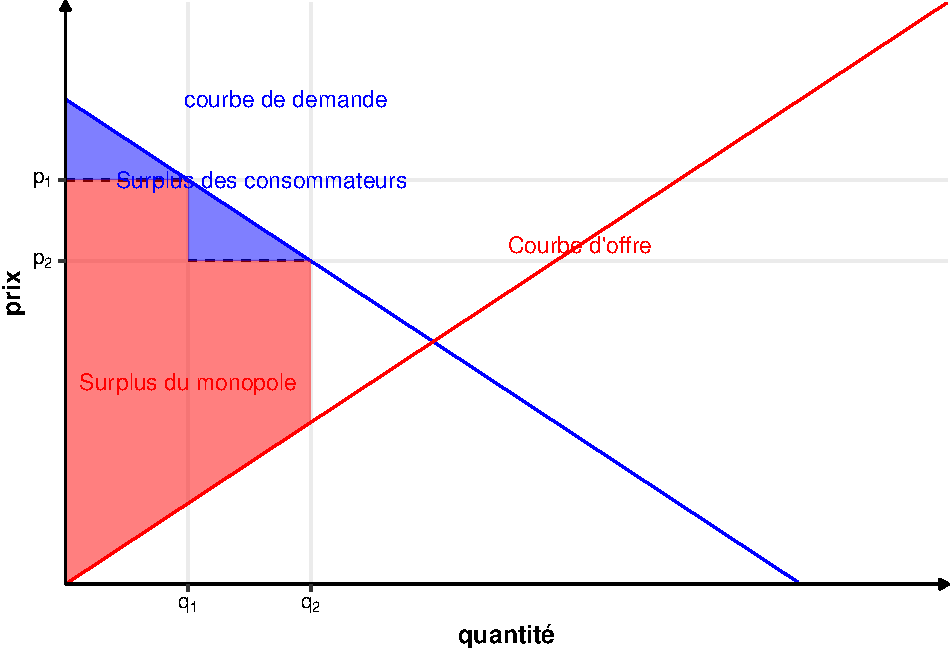
\includegraphics{_main_files/figure-latex/monopolediscri2degre-1.pdf}
\caption{\label{fig:monopolediscri2degre}Graphique avec une discrimination du deuxième degré. Les quantités inférieures à \(q_1\) sont vendues au prix \(p_1\), les suivantes au prix \(p_2\).}
\end{figure}

Le monopole ajuste les quantités seuils afin de maximiser son profit.
Il y a un nombre fini de seuils de dégressivité.
Plus il y a de seuils, plus on s'approche d'un situation de discrimination parfaite.

\hypertarget{discrimination-du-troisiuxe8me-degruxe9}{%
\subsection{Discrimination du troisième degré}\label{discrimination-du-troisiuxe8me-degruxe9}}

Il s'agit de faire payer un prix différent à chaque groupe de consommateur, en fonction des caractéristiques de leurs fonctions de demande.
Tous les membres d'un groupe payent donc le même prix, contrairement à la discrimination au premier degré.
Les groupes sont en général caractérisés par des propensions à payer différentes.
Il s'agit d'une segmentation des consommateurs.

\begin{example}[Discrimination au troisième degré]
Les tarifs jeunes de la SNCF, les tarifs familles.
Il est important de pouvoir identifier les groupes.
\end{example}

\emph{Question :} Comment répartir la production entre les différents groupes ?

\begin{enumerate}
\def\labelenumi{\arabic{enumi}.}
\tightlist
\item
  Quelle production totale ?
\item
  Quelle répartition ?
\end{enumerate}

\emph{Méthode :} On résout d'abord 2 en supposant que 1 est déjà résolu.
On obtient alors la répartition en fonction de la production totale.
Puis ou résout 1 à l'aide de la solution de 2.

On modélise le problème de la manière suivante :

\begin{itemize}
\tightlist
\item
  2 groupes A et B;
\item
  Avec des fonctions de demande inverses \(P_A(q_A)\) et \(P_B(q_B)\);
\item
  Une quantité \(q\) totale a été produite, qu'il faut répartir entre les 2 groupes : \(q=q_A+q_B\)
\end{itemize}

Le problème du monopole s'écrit :
\[
\max_{q_A, q_B} \pi(q_A, q_B) = q_AP_A(q_A) + q_BP_B(q_B) -C(q)
\]
La quantité totale \(q\) est fixée, donc le coût total l'est aussi et peut être supprimé du problème de maximisation.
On cherche donc juste à maximiser la recette totale :
\[
\max_{q_A, q_B} q_AP_A(q_A) + q_BP_B(q_B) 
\]
Avec \(q=q_A+q_B\), donc \(q_B=q-q_A\), le problème devient :
\[
\begin{array}{rl}
&\max_{q_A, 0\leq q_A\leq q} q_AP_A(q_A) + (q-q_A)P_B(q-q_A) \\
\Leftrightarrow &\max_{q_A, 0\leq q_A\leq q} R_A(q_A) + R_B(q-q_A) 
\end{array}
\]
La condition du premier ordre s'écrit :
\[
\begin{array}{rl}
&\frac{dR_A(q_A) + R_B(q-q_A) }{dq_A} = 0\\
\Leftrightarrow & R_{mA}(q_A) - R_{mB}(q-q_A) = 0\\
\Leftrightarrow & R_{mA}(q_A) = R_{mB}(q_B) 
\label{eq:cpo3e}
\end{array}
\]
L'équation \eqref{eq:cpo3e} nous dit que le monopole réparti la quantité totale produite de manière égaliser les recettes marginales entre les deux groupes.

Intuitivement, si la recette marginale issue du groupe A est supérieure à celle issue du groupe B (\(R_{mA}(q_A) > R_{mB}(q_B)\)), alors en diminuant la quantité \(q_B\) dans le groupe B et en la transférant au groupe A, le monopole perd \(R_{mB}(q_B)\) et gagne \(R_{mA}(q_A)\), donc la recette totale augmente et le profit aussi.
Inversement dans le cas opposé.
Il n'est donc pas intéressant de transférer la production d'un groupe vers un autre lorsque \(R_{mA}(q_A) = R_{mB}(q_B)\) (et seulement dans ce cas).

Maintenant que la répartition est résolue, il faut trouver la quantité totale produite.
Le problème devient maintenant :
\[
\max_{q_A, q_B} \pi(q_A, q_B) = q_AP_A(q_A) + q_BP_B(q_B) -C(q_A+q_B)
\]
La condition du premier ordre s'obtient maintenant en dérivant suivant \(q_A\) et \(q_B\) séparément :
\[
\begin{array}{rcl}
\frac{\partial\pi(q_A, q_B)}{\partial q_A} = 0&\Leftrightarrow& R_{mA}(q_A^*) = C_m(q_A^*+q_B^*)\\
\frac{\partial\pi(q_A, q_B)}{\partial q_B} = 0&\Leftrightarrow& R_{mB}(q_B^*) = C_m(q_A^*+q_B^*)\\
\end{array}
\]
Le monopole doit faire en sorte que le coût marginal de sa production totale soit égale à la recette marginale sur chacun des marchés.

\emph{Intuition :}
Le monopole doit égaliser la recette marginale sur les deux marchés.
Or le coût marginal dépend de la quantité \emph{totale} produite, pas de la répartition entre les marchés.
Si on est dans la situation telle que \(C_m(q)<R_{mA}(q_A)\), alors il y a la possibilité de faire du profit sur le marché A (et le marché B par conséquent).
Inversement, si \(C_m(q)>R_{mA}(q_A)\), alors le monopole fait des pertes.

\begin{remark}
On utilise bien \(C_m(q_A+q_B)\) et non \(C_m(q_A)\) ou \(C_m(q_B)\) car c'est bien la variation du coût total lorsqu'on augmente ``un peu'' \(q_A\) et \(q_B\) reste fixe.
\end{remark}

D'après l'équation \eqref{eq:rm}, on peut écrire :
\[
\begin{array}{crcl}
&R_{mA}(q_A^*) &=& R_{mB}(q_B^*)\\
\Leftrightarrow & P_A(q_A^*)\left(1-\frac{1}{\left|\varepsilon_{q/p_A}(q^*_A)\right|}\right) & = & P_B(q_B^*)\left(1-\frac{1}{\left|\varepsilon_{q/p_B}(q_B^*)\right|}\right)
\end{array}
\]
Sans perte de généralité, on peut supposer que \(P_A(q_A^*)> P_B(q_B^*)\).
On obtient alors que :
\[
1-\frac{1}{\left|\varepsilon_{q/p_A}(q_A^*)\right|} <1-\frac{1}{\left|\varepsilon_{q/p_B}(q_B^*)\right|}
\]
Autrement dit
\[
\left|\varepsilon_{q/p_B}(q_B^*)\right|>\left|\varepsilon_{q/p_A}(q^*_A)\right|
\]
Le prix est donc plus faible pour le groupe où l'élasticité prix de la demande est plus élevée.
Le prix est plus élevé pour le groupe avec l'élasticité la plus faible, les moins réactifs au prix.

\begin{example}
Les tarifs ``professionnels'' dans les transports (avion, train, etc).
Les professionnels sont moins sensibles au prix car leurs dates de voyage sont moins flexibles que celles des particuliers.
Leur élasticité prix est donc plus faible et leur prix plus élevés.
\end{example}

Des fonctions de demande inverse différentes associées à des élasticités prix de la demande différente aboutissent à des prix différents.

\hypertarget{oligopoles}{%
\chapter{Oligopoles}\label{oligopoles}}

On a vu jusqu'à présent deux cas extrêmes :

\begin{itemize}
\tightlist
\item
  La concurrence pure et parfaite :
  il y a une infinité d'entreprise infinitésimales sur un marché donné.
\item
  Le monopole : il y a une seule entreprise sur un marché donné.
\end{itemize}

Dans les deux cas, l'entreprise ou les entreprises n'ont pas à se préoccuper des autres entreprises.
Dans le cas du monopole, parce qu'il n'y en a pas.
Dans le cas de la CPP, l'entreprise observe le prix du marché et prend sa décision en fonction de ce prix, et uniquement de ce prix.
Les actions des autres entreprises ne l'influence pas.

On considère maintenant la situation où il n'y a plus une seule ou une infinité d'entreprises, mais plusieurs, qui sont en situation d'\emph{interactions stratégiques}.
Les décisions de chaque acteur dépend des décisions des autres acteurs (ou des anticipations de ces décisions).\\
On parle de \emph{duopole} dans le cas où le marché compte deux entreprises et d'\emph{oligopole} dans le cas où il compte plus que deux entreprises.\\
Les entreprises peuvent se faire concurrence de différentes manières :

\begin{itemize}
\tightlist
\item
  En quantité, concurrence dite à la \emph{Cournot} ;
\item
  En prix, concurrence à la \emph{Bertrand} ;
\item
  En prenant une situation de leader ou de follower, à la \emph{Stackelberg} ;
\item
  En format une entente, dans un \emph{cartel} ;
\item
  Dans une concurrence spatiale, à la \emph{Hotelling}.
\end{itemize}

Nous verrons dans ce cours les concurrences à la Cournot et à la Stackelberg, ainsi que les cartels.

\hypertarget{duopole-uxe0-la-cournot}{%
\section{Duopole à la Cournot}\label{duopole-uxe0-la-cournot}}

\hypertarget{introduction}{%
\subsection{Introduction}\label{introduction}}

On considère deux entreprises sur le même marché qui doivent choisir les quantités à produire, sans connaître la quantité choisie par l'autre (= décision simultanée).\footnote{Même marché : bien unique et prix unique.}
Le prix est déterminé par la quantité \emph{totale} produite par les deux entreprises et la fonction de demande sur le marché.

Chaque entreprise est caractérisée par une quantité produite et un coût :

\begin{itemize}
\tightlist
\item
  Entreprise 1 : quantité \(q_1\) produite au coût \(C_1(q_1)\) ;
\item
  Entreprise 2 : quantité \(q_2\) produite au coût \(C_2(q_2)\).
\end{itemize}

Les fonctions de coût sont \textbf{différentes} entre les deux entreprises, contrairement au cas du monopole discriminant au troisième degré, où l'on considérait \(C(q_1+q_2)\).

La fonction de demande inverse sur le marché est \(P(q_1+q_2)\).
C'est différent du monopole discriminant où il y avait une fonction de demande par segment.

On a donc les fonctions de profit:
\[
\begin{array}{rcl}
\pi_1(q_1, q_2) &=& P(q_1+q_2)\cdot q_1-C_1(q_1)\\
\pi_2(q_1, q_2) &=& P(q_1+q_2)\cdot q_2-C_2(q_2)
\end{array}
\]
L'action d'une entreprise a des conséquences sur le profit réalisé par l'autre entreprise, même si celle-ci ne fait rien.
En particulier, si \(q_1\) augmente, alors le prix du marché diminue, au travers de la fonction de demande inverse \(P\), et donc le profit de l'entreprise 2, \(\pi_2\), diminue, et réciproquement si \(q_2\) augmente.
Il y a donc un conflit d'intérêt entre les producteurs.
Chaque entreprise doit anticiper l'action de l'autre et réagir à cette anticipation le mieux possible.

\emph{Question :} Peut-il y avoir un équilibre dans cette situation ?

\hypertarget{formalisation-du-probluxe8me}{%
\subsection{Formalisation du problème}\label{formalisation-du-probluxe8me}}

\hypertarget{expression-des-profits}{%
\subsubsection{Expression des profits}\label{expression-des-profits}}

On a des profits :
\[
\begin{array}{rcl}
\pi_1(q_1, q_2) &=& P(q_1+q_2)\cdot q_1-C_1(q_1)\\
\pi_2(q_1, q_2) &=& P(q_1+q_2)\cdot q_2-C_2(q_2)
\end{array}
\label{eq:profitcournot}
\]

Supposons que l'entreprise 1 \emph{croit} que l'entreprise 2 va produire \(q_2^a\).
Quelle est sa production optimale ?
Son problème de maximisation est :
\[
\max_{q_1} \pi_1(q_1, q_2^a) =  q_1P(q_1+q_2^a)-C_1(q_1)
\]
On peut déduire de ce problème d'optimisation la \emph{fonction de réaction} \(q_1(q_2^a)=f_1(q_2^a)\) qui maximise \(\pi_1(q_1)\) en fonction de la production anticipée \(q_2^a\) de l'entreprise 2.\footnote{La fonction de réaction est parfois aussi connue sous le nom de \emph{fonction de meilleure réponse}.}
La fonction de réaction \(f_1(q_2^a)\) donne la valeur de \(q_1\) qui maximise le profit quand l'entreprise 2 produit \(q_2^a\).

De la même manière, l'entreprise 2 cherche à maximiser \(\pi_2\) en fonction de la production anticipée \(q_1^a\) de l'entreprise 1.
Son programme est :
\[
\max_{q_2} \pi_2(q_1^a, q_2) =  q_1P(q_1^a+q_2)-C_2(q_2)
\]
Elle aura également une fonction de réaction \(q_2(q_1^a)=f_2(q_1^a)\).

\hypertarget{forme-des-fonctions-de-ruxe9action}{%
\subsubsection{Forme des fonctions de réaction}\label{forme-des-fonctions-de-ruxe9action}}

Si l'entreprise \(i\) pense que l'entreprise \(j\) ne va rien produire, alors elle se trouve dans une situation de monopole et se comporte comme tel.
Elle produit de manière à égaliser coût marginal et recette marginale (\(R_{im}=C_{im}\)).

Si l'entreprise \(i\) pense que l'entreprise \(j\) va produire \(q_j^a>0\), alors elle est en monopole sur le \textbf{reste} de la demande.
Cette dernière correspond à la demande totale décalée de \(q_j^a>0\) vers la gauche.
Le croisement entre recette marginale et coût marginal se fait donc à un niveau plus faible qu'auparavant.

Plus l'entreprise \(i\) pense que l'entreprise \(j\) va produire une grande quantité, plus elle aura intérêt à réduire son offre.
\(q_i\) est décroissante en \(q_j^a\)

\begin{figure}
\centering
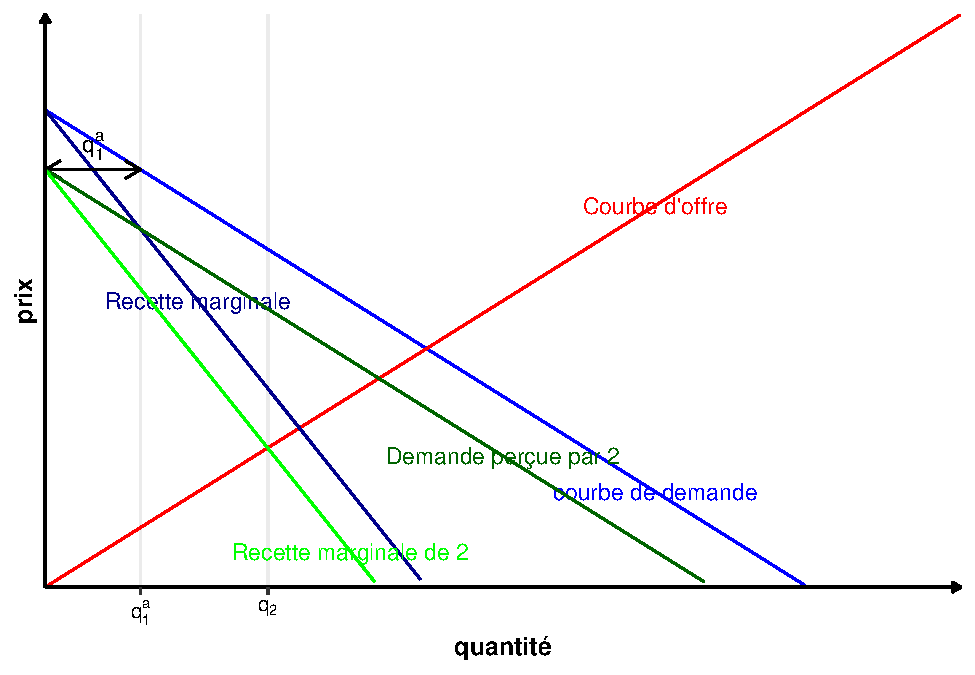
\includegraphics{_main_files/figure-latex/oligodemande-1.pdf}
\caption{\label{fig:oligodemande}Représentation de la demande perçue par l'entreprise 2 anticipant une offre \(q_1^a\) par l'entreprise 1.}
\end{figure}

\hypertarget{caractuxe9risation-de-luxe9quilibre}{%
\subsubsection{Caractérisation de l'équilibre}\label{caractuxe9risation-de-luxe9quilibre}}

Un équilibre \((q_1^a, q_2^a)\) doit être tel qu'aucune des deux entreprises n'ait intérêt à dévier unilatéralement :
\[
\begin{array}{rcl}
\pi_1(q_1^a, q_2^a) &\geq& \pi_1(q_1, q_2^a)\quad \forall q_1\\
\pi_2(q_1^a, q_2^a) &\geq& \pi_2(q_1^a, q_2)\quad \forall q_2
\end{array}
\]
Au point \(q_1^a\) et \(q_2^a\), aucune entreprise n'a intérêt à dévier unilatéralement de l'équilibre.
Les décisions prises sont mutuellement compatibles.
Chaque entreprise donne sa meilleure réponse à la meilleure réponse de l'autre.
C'est ce qu'on appelle un \textbf{équilibre de Nash} : un équilibre où personne n'a intérêt à dévier unilatéralement.

Dans le cas du duopole à la Cournot, chaque entreprise doit choisir la quantité qui maximise son profit étant donné le choix de l'autre entreprise.
Chaque entreprise est donc sur sa fonction de réaction.
L'équilibre est donc à l'intersection des fonctions de réactions des deux entreprises :
\[
\begin{array}{rcl}
q_1^a&=&f_1(q_2^a)\\
q_2^a&=&f_2(q_1^a)
\end{array}
\]

\begin{figure}
\centering
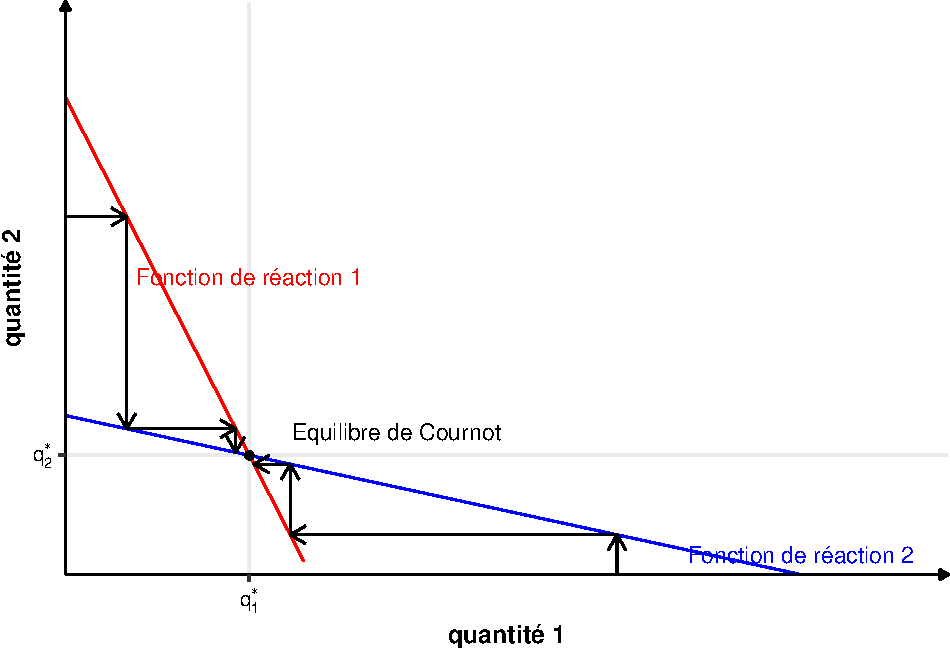
\includegraphics{_main_files/figure-latex/oligoreaction-1.pdf}
\caption{\label{fig:oligoreaction}Représentation d'un équilibre de Cournot où les fonctions de réaction convergent vers le point d'équilibre.}
\end{figure}

L'équilibre n'est pas nécessairement stable.
La stabilité dépend de la pente des fonctions de réactions.

\begin{figure}
\centering
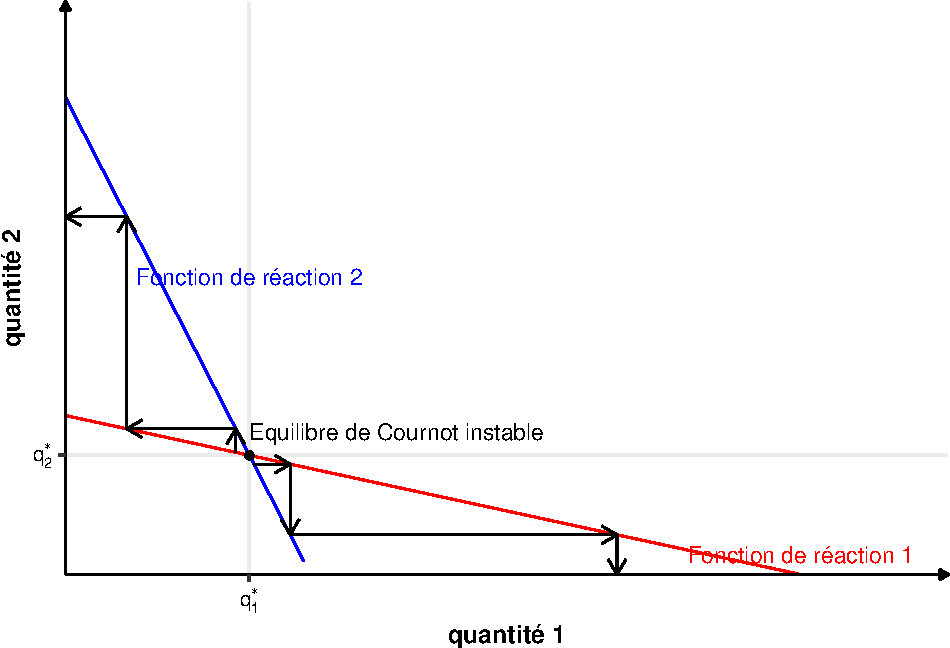
\includegraphics{_main_files/figure-latex/oligoreactioninstable-1.pdf}
\caption{\label{fig:oligoreactioninstable}Représentation d'un équilibre de Cournot où les fonctions de réaction divergent du point d'équilibre. Equilibre instable}
\end{figure}

\hypertarget{exemple}{%
\subsection{Exemple}\label{exemple}}

\hypertarget{donnuxe9es-du-probluxe8me}{%
\subsubsection{Données du problème}\label{donnuxe9es-du-probluxe8me}}

Prenons les fonctions suivantes :

\[
\begin{array}{l}
P(q_1+q_2) = a - b(q_1+q_2)\\
C_1(q_1) = cq^2_1 \\
C_2(q_2) = cq^2_2 \\
\end{array}
\]

\hypertarget{profits}{%
\subsubsection{Profits}\label{profits}}

On en déduit les profits :

\[
\begin{array}{rcl}
\pi_1(q_1, q_2) &=& \left(a-b(q_1+q_2)\right)q_1-cq_1^2\\
\pi_2(q_1, q_2) &=& \left(a-b(q_1+q_2)\right)q_2-cq_2^2
\end{array}
\]

\hypertarget{fonctions-de-ruxe9action}{%
\subsubsection{Fonctions de réaction}\label{fonctions-de-ruxe9action}}

Calculons la fonction de réaction de l'entreprise 1.
Son profit est :
\[
\pi_1(q_1, q_2^a) = aq_1-bq_1^2-bq_2^aq_1-cq_1^2 = (a-bq_2^a)q_1-(b+c)q_1^2
\]

La condition du premier ordre suivant \(q_1\) s'écrit (ici \(q_2^a\) est considéré comme une donnée par l'entreprise 1) :

\[
\begin{array}{crcl}
&\frac{\partial \pi_1}{\partial q_1}&=&0\\
\Leftrightarrow & (a-bq_2^a)-2(b+c)q_1^* &=& 0\\
\Leftrightarrow & q_1^* &=& \frac{(a-bq_2^a)}{2(b+c)}
\label{eq:FR1}
\end{array}
\]

On calcule de la même manière (i.e., en utilisant la condition du premier ordre sur les profits de l'entreprise 2) la fonction de réaction de l'entreprise 2 et on obtient par symétrie du problème une légère réécriture de l'équation \eqref{eq:FR1}:

\[
q_2^* = \frac{(a-bq_1^a)}{2(b+c)}
\]

La symétrie du problème provient du fait que les deux entreprises ont exactement la même fonction de coût.
Ce \emph{n'est pas le cas en général}.
Si dans un problème les fonctions de coût sont identiques, alors vous pouvez faire les calculs pour une seule entreprise et déduire simplement les résultats pour la seconde.

\hypertarget{equilibre-de-cournot}{%
\subsubsection{Equilibre de Cournot}\label{equilibre-de-cournot}}

Quel est alors l'équilibre de Cournot ?

On doit avoir :
\[
\begin{array}{rcl}
f_1(q_2^*) &=& q_1^*\\
f_2(q_1^*) &=& q_2^*\\
\end{array}
\]
Autrement dit :
\[
\begin{array}{rcl}
q_1^* &=& \frac{(a-bq_2^*)}{2(b+c)} \\
q_2^* &=&\frac{(a-bq_1^*)}{2(b+c)}\\
\end{array}
\]
On résout le système et on obtient :
\[
q_1^*=q_2^* = \frac{a}{3b+2c}
\]

Quand le problème est symétrique, les deux entreprises en compétition à la Cournot produisent la même quantité de bien.

\hypertarget{une-intuition-graphique-les-courbes-disoprofit}{%
\subsection{Une intuition graphique : les courbes d'isoprofit}\label{une-intuition-graphique-les-courbes-disoprofit}}

On peut aussi aborder le problème à l'aide d'une intuition graphique.
Il s'agit de tracer les courbes d'\emph{isoprofit} des entreprises.

\begin{definition}[Courbe d'isoprofit]
Les courbes d'isoprofit est l'ensemble des couples de quantités \((q_1, q_2)\) qui permettent à une entreprise d'atteindre un niveau de profit donné.
\end{definition}

Reprenons l'expression générale des profits de l'équation \eqref{eq:profitcournot}.
\[
\begin{array}{rcl}
\pi_1(q_1, q_2) &=& q_1P(q_1+q_2)-C_1(q_1)\\
\pi_2(q_1, q_2) &=& q_2P(q_1+q_2) -C_2(q_2)
\end{array}
\]
La courbe d'isoprofit pour une valeur \(\pi_1\) \textbf{donnée et fixe} est :
\[
\pi_1 = q_1P(q_1+q_2)-C_1(q_1)
\]
L'équation ci-dessus définit implicitement une fonction \(q_1=I_\pi(q_1, \pi_1)\) qui permet de représenter la courbe d'isoprofit dans un graphique \((q_1,q_2)\), tout comme la fonction de réaction définit une fonction courbe \(q_2(q_1)\) pour l'entreprise 1.
La courbe de la fonction de réaction de 1 coupe la courbe d'isoprofit de 1 en son maximum.

\begin{figure}
\centering
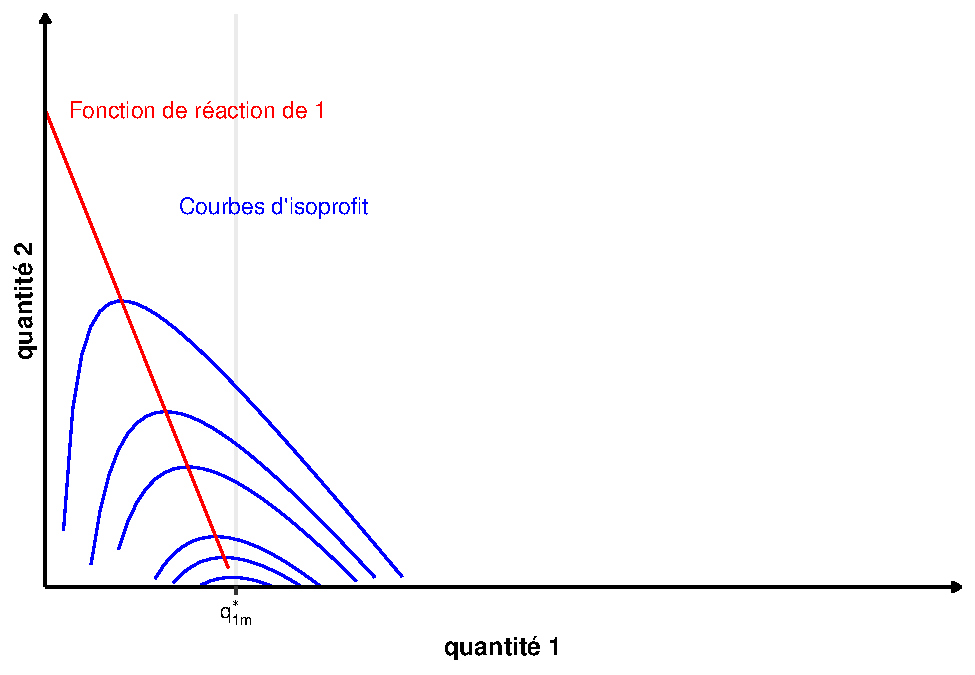
\includegraphics{_main_files/figure-latex/isoprofit1-1.pdf}
\caption{\label{fig:isoprofit1}Courbes d'isoprofit et fonction de réaction de l'entreprise 1}
\end{figure}

Sur la figure \ref{fig:isoprofit1}, le profit est croissant en descendant vers le bas sur les courbes d'isoprofit, autrement dit, les courbes d'isoprofit les plus basses représentent les profits les plus élevés.
Le maximum du profit est atteint lorsque l'entreprise 1 est en monopole.
La quantité produite est alors \(q_m^*\) est le profit \(\pi_m^*\).

\begin{figure}
\centering
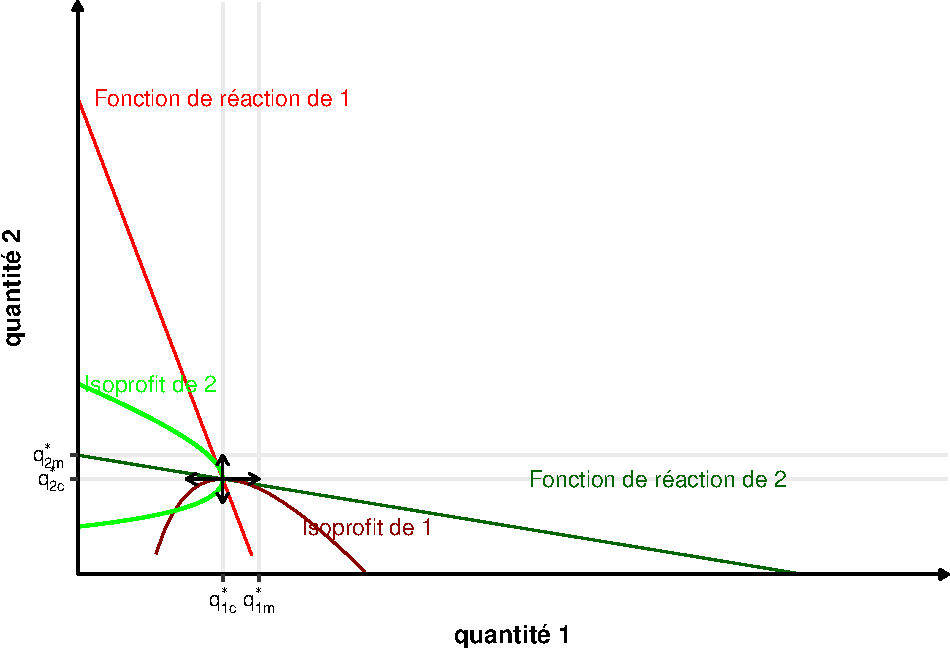
\includegraphics{_main_files/figure-latex/isoprofitCournot-1.pdf}
\caption{\label{fig:isoprofitCournot}Courbes d'isoprofits et fonctions de réactions des entreprises en équilibre de Cournot Nash.}
\end{figure}

\hypertarget{extension-oligopole-uxe0-la-cournot}{%
\subsection{Extension : oligopole à la Cournot}\label{extension-oligopole-uxe0-la-cournot}}

On étend l'analyse à \(N\) entreprises qui produisent un bien \emph{homogène}.
Comme ce bien est homogène, le prix est unique sur le marché.
Chaque entreprise \(i\) choisit une quantité \(q_i\geq 0\) et les produit à un coût de production \(C_i(q_i)\).
La production totale sur le marché est \(q=\sum_i q_i\).
La fonction de demande inverse sur le marché \(P(q)\) dépend de la production \emph{globable} \(q\).

Le profit de chaque entreprise s'écrit :
\[
\pi(q_i, q_{-i}) = q_iP(q) -C_i(q_i)
\]
Où \(q_{-i}\) est la somme de la production de toute les entreprises autres que l'entreprise \(i\).
Autrement dit \(q=q_i+q_{-i}\).

Le programme de maximisation d'une entreprise \(i\) s'écrit :
\[
\max_{q_i}\pi(q_i, q_{-i}) = q_iP(q) -C_i(q_i)
\]

La condition du premier ordre est telle que :

\[
\begin{array}{crcl}
&\frac{\partial \pi_i}{\partial q_i}(q^*) &=& 0\\
\Leftrightarrow & \frac{\partial  \left(q_iP(q_i+q_{-i}) -C_i(q_i)\right)}{\partial q_i}(q^*) &= &0\\
\Leftrightarrow & P(q^*) + q_i\frac{\partial  P}{\partial q}(q^*) -C_{im}(q_i^*)&= &0\\
\Leftrightarrow & P(q^*) - C_{im}(q_i^*)&= &-q_i^*\frac{\partial  P}{\partial q}(q^*) \\
\Leftrightarrow & \frac{P(q^*)-C_{im}(q_i^*)}{P(q^*)}&= &-\frac{q_i^*}{P(q^*)}\frac{\partial  P}{\partial q}(q^*) \\
\Leftrightarrow & \frac{P(q^*) -C_{im}(q_i)^*}{P(q^*)}&= &-\frac{q^*}{P(q^*)}\frac{\partial  P}{\partial q}(q^*)\frac{q_i^*}{q^*} \\
\Leftrightarrow & \frac{P(q^*) - C_{im}(q_i^*)}{P(q^*)}&= &S_i\frac{1}{\left|\varepsilon_{q/p}(q^*)\right|}
\end{array}
\]
(La dérivée de la fonction de demande suivant le prix est négative).

On obtient le \emph{markup-pricing} que peut appliquer un producteur en situation d'oligopole à la Cournot.
\[\frac{P(q^*) -C_{im}(q_i^*)}{P(q^*)}= \frac{S_i}{\left|\varepsilon_{q/p}(q^*)\right|}\]
La possibilité de fixer un prix au-dessus du coût marginal dépend de la part de marché de l'entreprise.

\begin{remark}
En monopole, \(S_i=1\), on retrouve alors bien :
\[\frac{P(q) -C_{im}(q)}{P(q)}= \frac{1}{\left|\varepsilon_{q/p}(q)\right|}\]

En concurrence pure et parfaite \(S_i\to 0\), donc \(\frac{P(q) -C_{im}(q_i)}{P(q)}\to 0\), ce qui implique bien que \(C_{mi}(q_i)\to P(q)\).
On retrouve ainsi le résultat \(P(q^*)=C_m(q^*)\).
\end{remark}

\hypertarget{indice-de-lerner}{%
\subsection{Indice de Lerner}\label{indice-de-lerner}}

\emph{Rappel :} En monopole, l'indice de Lerner est :
\[L=\frac{P(q_m^*)-C_m(q_m^*)}{P(q_m^*)} = \frac{1}{\left|\varepsilon_{q/p}(q_m^*)\right|}\]

\begin{definition}[Indice de Lerner]
En oligopole à la Cournot avec \(n\) producteurs, on définit l'indice de Lerner par :
\[L = \sum_{i=1}^nS_iL_i\]
où \(S_i=q_i/q\) est la \emph{part de marché} de l'entreprise \(i\) et \(L_i\) est l'indice de Lerner propre à un producteur.
\end{definition}

\(q\) est la production totale \(q=\sum_{i=1}^N q_i\).
Notons \(q=(q_i, q_{-i})\) le vecteur donnant les quantités produites par chaque producteur.
\(q_i\) est la quantité produite par le producteur \(i\), \(q_{-i}=(q_1,\dots,q_{i-1}, q_{i+1}, \dots,q_N)\) est le vecteur de toutes les unités produites par les autres producteurs.

Exprimons maintenant l'indice de Lerner d'un producteur.
\[
\begin{array}{rcl}
L_i &=&\frac{1}{\left|\varepsilon_{q/p}(q_i, q_{-i})\right|}=\frac{P(q^*)-C_{im}(q_i^*)}{P(q^*)}\\
&=&\frac{1}{\left|\frac{1}{\frac{\partial P}{\partial q}(q)}\frac{P(q)}{q_i}\right|}\\
&=&\frac{1}{\left|\frac{1}{\frac{\partial P}{\partial q}(q)}\frac{P(q)}{q}\frac{q}{q_i}\right|}\\
&=&\frac{1}{\left|\frac{1}{\frac{\partial P}{\partial q}(q)}\frac{p}{q}\right|}\frac{q_i}{q}\\
&=&\frac{S_i}{\left|\varepsilon_{q/p}(q)\right|}\\
\end{array}
\]

On peut donc réécrire l'indice de Lerner uniquement en fonction de l'élasticité de la demande à l'équilibre et des parts de marchés de chaque producteur :
\[
L=\frac{1}{\left|\varepsilon_{q/p}(q^*)\right|}\sum_{i=1}^NS_i^2
\]

\hypertarget{indice-de-concentration-du-marchuxe9}{%
\subsection{Indice de concentration du marché}\label{indice-de-concentration-du-marchuxe9}}

\begin{definition}[Indice de Hirschman-Herfindahl (HHI)]
\protect\hypertarget{def:HHI}{}\label{def:HHI}L'indice de Hirschman-Herfindahl est la somme des carrés des part de marchés.
\[HHI = \sum_{i=1}^NS_i^2\]
C'est aussi la différence moyenne entre le coût marginal de production et le prix, multiplié par l'élasticité prix de la demande à l'optimum.
Autrement dit, la moyenne des \(L_i\) pondéré par les parts de marché.
\end{definition}

\[
 \begin{array}{rcl}
 \sum_{i=1}^{N}\frac{P(q) -C_{im}(q_i)}{P(q)}S_i &=&\sum_{i=1}^{N} \frac{S_i}{\left|\varepsilon_{q/p}(q^*)\right|}S_i \\
 &=&\frac{1}{\left|\varepsilon_{q/p}(q^*)\right|}\sum_{i=1}^NS_i^2\\
 &=&\frac{HHI}{\left|\varepsilon_{q/p}(q^*)\right|}
 \end{array}
 \]

\emph{Interprétation :}\\
Imaginons que toutes les \(N\) entreprises sont identiques (elles ont la même fonction de coût).
Elles produisent alors la même quantité optimale à l'équilibre.
Leur part de marché est donc \(S_i=1/N\).
Le HHI vaut :
\[
\begin{array}{rcl}
HHI&=&\sum_{i=1}^NS_i^2\\
&=&\sum_{i=1}^N\frac{1}{N^2}\\
&=&\frac{N}{N^2} \\
&=&\frac{1}{N}
\end{array}
\]
Le HHI correspond à l'inverse du nombre du nombre d'entreprise qui serait identique sur le marché et donnerait le même écart moyen entre coût marginal et prix.
Plus le HHI est proche de 1, plus on se rapproche du monopole.

Le HHI est utilisé par les autorités de la concurrence pour évaluer les effets sur les prix de fusions d'entreprises.
Elles peuvent interdire des fusions qui augmenteraient trop fortement le HHI.

\hypertarget{duopole-uxe0-la-stackelberg}{%
\section{Duopole à la Stackelberg}\label{duopole-uxe0-la-stackelberg}}

\hypertarget{introduction-1}{%
\subsection{Introduction}\label{introduction-1}}

Il n'y a plus de symétrie des entreprises dans un duopole à la Stackelberg.
Une entreprise, dite \emph{leader}, prend ses décisions avant l'entreprise dite \emph{follower}.
L'entreprise leader connaît les caractéristiques de l'entreprise follower et peut ainsi calculer sa fonction de réaction.
Elle va donc en tenir compte dans ses décisions.
On considère ici qu'il n'y a que deux périodes de décisions.

\hypertarget{ruxe9solution-graphique}{%
\subsection{Résolution graphique}\label{ruxe9solution-graphique}}

Le leader doit choisir sa quantité \(q_1\) de façon à être sur la courbe d'isoprofit la plus basse possible compatible avec la fonction de réaction de l'entreprise follower.
Il va donc se placer sur la courbe d'isoprofit tangente à la fonction de réaction du follower.

\begin{figure}
\centering
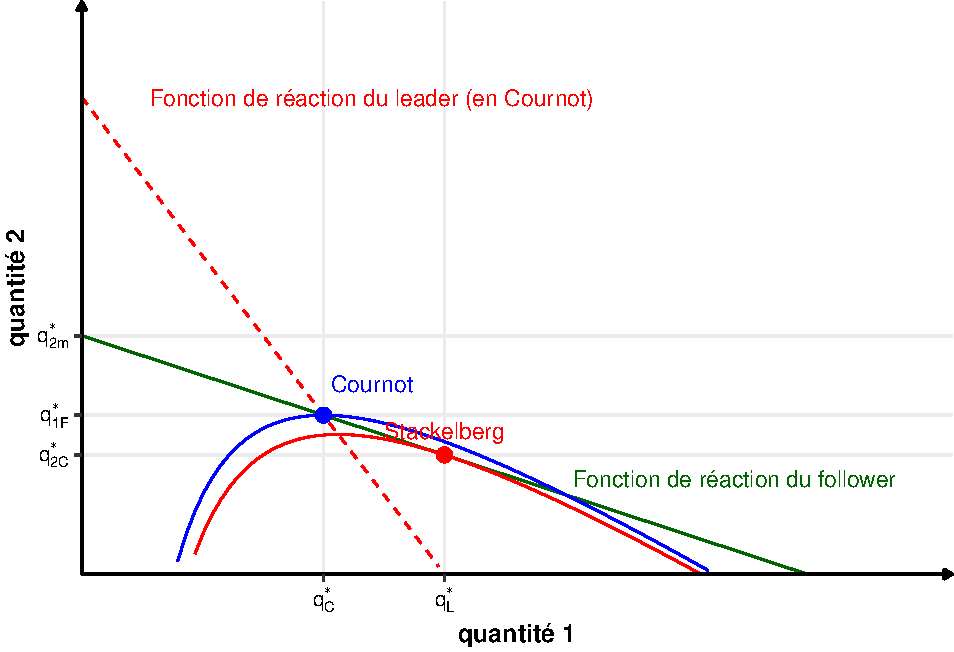
\includegraphics{_main_files/figure-latex/equilibreStackelberg-1.pdf}
\caption{\label{fig:equilibreStackelberg}Courbes d'isoprofits du leader et fonctions de réactions des entreprises en équilibre de Stackelberg.}
\end{figure}

Sur la figure \ref{fig:equilibreStackelberg}, on voit que le profit du leader est plus important en Stackelberg qu'en Cournot (et l'inverse pour le follower).
Les quantités produites par l'entreprise leader sont plus importantes en Stackelberg qu'en Cournot, mais celles du follower sont plus faibles.
La somme des deux est plus importante (\(q_{1C}^*+q_{2C}^*<q_{L}^*+q_{F}^*\)).
Le prix sera donc plus faible pour les consommateurs.

\hypertarget{exemple-1}{%
\subsection{Exemple}\label{exemple-1}}

\hypertarget{donnuxe9es-du-probluxe8mes}{%
\subsubsection{Données du problèmes}\label{donnuxe9es-du-probluxe8mes}}

Notons les variables et fonctions du leader avec un indice \(L\) et celles du follower avec un indice \(F\).

Gardons une fonction de demande linéaire.

\[
P(q_L+q_F) = a - b(q_L+q_F)
\]

Supposons, afin de simplifier les calculs, que les coûts marginaux sont nuls.

\hypertarget{profits-1}{%
\subsubsection{Profits}\label{profits-1}}

On en déduit les profits :

\[
\begin{array}{rcl}
\pi_L(q_L, q_F) &=& \left(a-b(q_L+q_F)\right)q_L\\
\pi_F(q_L, q_F) &=& \left(a-b(q_L+q_F)\right)q_F
\end{array}
\]

\hypertarget{fonction-de-ruxe9action-de-lentreprise-follower}{%
\subsubsection{Fonction de réaction de l'entreprise follower}\label{fonction-de-ruxe9action-de-lentreprise-follower}}

Calculons la fonction de réaction de l'entreprise follower.
La condition du premier ordre suivant \(q_F\) s'écrit (ici \(q_L\) est considéré comme une donnée par l'entreprise 1) :

\[
\begin{array}{crcl}
&\frac{\partial \pi_F}{\partial q_F}&=&0\\
\Leftrightarrow & (a-bq_L)-2bq_F^* &=& 0\\
\Leftrightarrow & q_F^* &=& \frac{a-bq_L}{2b}
\label{eq:FRFollower}
\end{array}
\]

\hypertarget{maximisation-de-lentreprise-leader}{%
\subsubsection{Maximisation de l'entreprise leader}\label{maximisation-de-lentreprise-leader}}

Comme l'entreprise leader connaît la fonction de réaction de l'entreprise follower (donnée par l'équation \eqref{eq:FRFollower}), elle peut l'intégrer à sa propre fonction de profit :

\[
\begin{array}{rcl}
\pi_L(q_L, q_F^*) &=& \left(a-b(q_L+q_F^*(q_L))\right)q_L\\
 &=& \left(a-b\left(q_L+\frac{a-bq_L}{2b}\right)\right)q_L\\
 &=& \frac{a}{2}q_L-\frac{b}{2}q_L^2
\end{array}
\]

La condition de premier ordre du leader est :

\[
\begin{array}{crcl}
&\frac{\partial \pi_L}{\partial q_L}&=&0\\
\Leftrightarrow & \frac{a}{2}-bq_L^* &=& 0\\
\Leftrightarrow & q_L^* &=& \frac{a}{2b}
\end{array}
\]

On en déduit qu'à l'équilibre de Stackelberg, le follower produit :
\[
q_F^*=\frac{a}{4b}
\]

L'entreprise leader produit plus que l'entreprise follower.
Elle profite de son pouvoir sur la seconde entreprise pour cela.
Si on calcule le profit, on verra que le profit de l'entreprise leader est plus important que celui de l'entreprise follower si elles sont exactement symétriques, en dehors de leur prises de décisions.

\hypertarget{cartels-et-collusions}{%
\section{Cartels et collusions}\label{cartels-et-collusions}}

\hypertarget{introduction-2}{%
\subsection{Introduction}\label{introduction-2}}

En duopoles / oligopoles de Cournot ou de Stackelberg, les entreprises ne coopèrent pas entre elles :

\begin{itemize}
\tightlist
\item
  Elles sont en concurrence ;
\item
  Elles agissent indépendamment les unes des autres.
\end{itemize}

\emph{Question :}\\
Que se passe-t-il si elles peuvent s'entendre ?
Par exemple, que se passe-t-il si elle peuvent passer un accord sur la quantité à produire.

\emph{Résultats :}\\
Les quantités mises sur le marché vont diminuer, et le prix du marché va augmenter.
C'est donc néfaste pour les consommateurs.
La raison est que le cartel se comporte exactement comme un monopole, puis partage les bénéfices.

\hypertarget{raisonnement-graphique}{%
\subsection{Raisonnement graphique}\label{raisonnement-graphique}}

\begin{figure}
\centering
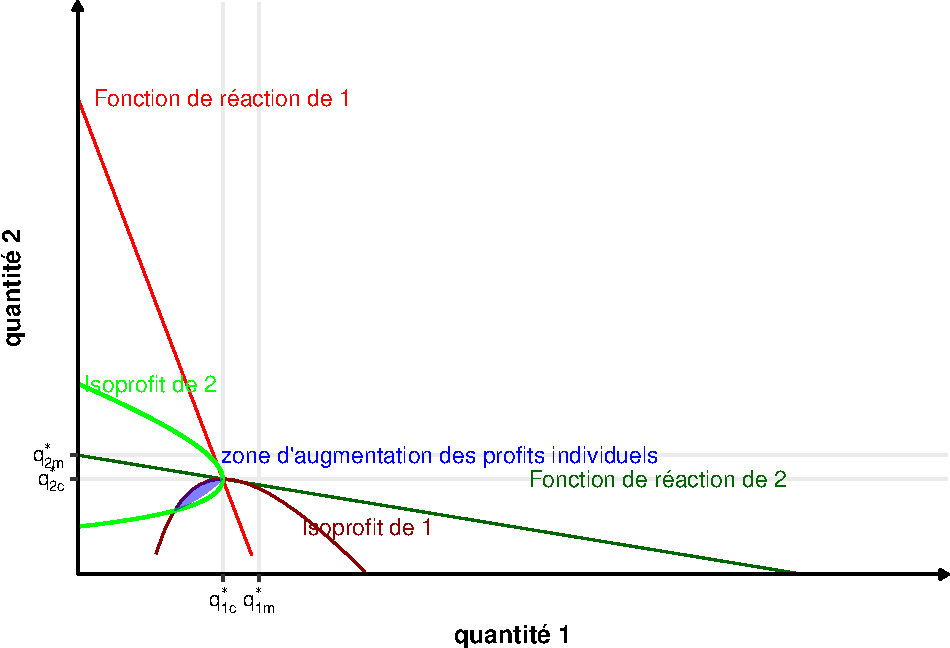
\includegraphics{_main_files/figure-latex/cartel-1.pdf}
\caption{\label{fig:cartel}Zone d'amélioration mutuellement bénéfique.}
\end{figure}

\hypertarget{ruxe9solution-analytique}{%
\subsection{Résolution analytique}\label{ruxe9solution-analytique}}

\hypertarget{iduxe9e}{%
\subsubsection{Idée}\label{iduxe9e}}

L'idée derrière la résolution analytique du problème du cartel est de considérer que le cartel se comporte comme un monopole avec 2 centres de productions.
Le cartel choisit la quantité globale produite et la répartition entre les entreprises.
C'est un raisonnement très similaire à un monopole discriminant au troisième degré.

\hypertarget{profits-2}{%
\subsubsection{Profits}\label{profits-2}}

Le profit global du cartel s'écrit :
\[
\pi_c=qP(q)-C_A(q_A)-C_B(q_B)=(q_A+q_B)P(q_A+q_B)-C_A(q_A)-C_B(q_B)
\]
Où \(q=q_A+q_B\).
Le profit est maximisé lorsque les dérivées partielles suivant chacune des quantités sont nulles (condition du premier ordre), c'est-à-dire lorsque \(\frac{\partial\pi_C}{\partial q_A}=0\) et \(\frac{\partial\pi_C}{\partial q_B}=0\).
\[
\frac{\partial\pi_C}{\partial q_A} = P(q) + q\frac{\partial P}{\partial q}(q_A)-\frac{\partial C_A}{\partial q_A}(q_A)
\]
On a \(P(q) + q\frac{\partial P}{\partial q}=R_m(q)\) est la recette marginale totale du cartel.
\(\frac{\partial C_A}{\partial q_A}=C_{mA}\) est le coût marginal de l'entreprise A.\\
On peut réécrire la dérivée du profit total suivant la quantité produite par l'entreprise A :
\[
\frac{\partial\pi_C}{\partial q_A} = R_m(q)  - C_{mA}(q_A)
\]
En utilisant le même raisonnement, on a pour l'entreprise B :
\[
\frac{\partial\pi_C}{\partial q_B} = R_m(q)  - C_{mB}(q_B)
\]

\hypertarget{optimalituxe9-pour-le-cartel}{%
\subsubsection{Optimalité pour le cartel}\label{optimalituxe9-pour-le-cartel}}

A l'optimum pour le cartel, on a donc :
\[R_m(q) = C_{mA}(q_A) = C_{mB}(q_B)\]
Le cartel égalise la recette marginale \emph{totale} aux coûts marginaux de chacune des deux entreprises.

\emph{Remarque :} Le cartel ne va pas forcément donner à produire la même quantité à chaque entreprise.
La répartition dépend des coûts marginaux respectifs.
Si les coûts marginaux sont identiques, les productions seront identiques.

\emph{Intuition :} Supposons que la quantité totale produite est fixée.
Supposons aussi que \(C_{mA}(q_A)>C_{mB}(q_B)\).\\
Alors, en transférant la production d'une unité de l'entreprise A vers l'entreprise B, le coût diminue de \(C_{mA}(q_A)\) et augmente de \(C_{mB}(q_B)\).
Il diminue donc au total, tout en maintenant la même quantité totale produite.\\
Autrement dit, tant que \(C_{mA}(q_A)\neq C_{mB}(q_B)\), il est possible de diminuer le coût total de production d'une quantité donnée en répartissant celle-ci différemment entre les entreprises.

\hypertarget{optimalituxe9-pour-une-entreprise}{%
\subsubsection{Optimalité pour une entreprise}\label{optimalituxe9-pour-une-entreprise}}

\emph{Question :} Prenons l'entreprise A, a-t-elle intérêt à rester dans le cartel (et à respecter la répartition donnée par celui-ci) ?

Le profit de l'entreprise A s'écrit :
\[
\pi_A=q_AP(q)-C_A(q_A)=q_AP(q_A+q_B)-C_A(q_A)
\]
La dérivée du profit s'écrit donc :
\[
\frac{\partial\pi_A}{\partial q_A}(q_A)=P(q_A+q_B)+q_A\frac{\partial P}{\partial q}(q_A)-C_{mA}(q_A)
\]
La condition d'optimalité du cartel suivant \(q_A\) donne :
\[
\begin{array}{crcl}
& P(q_A^*+q_B^*) + (q_A^*+q_B^*)\frac{\partial P}{\partial q}(q_A^*)-\frac{\partial C_A}{\partial q_A}(q_A^*)& = &0\\
\Leftrightarrow &  P(q_A^*+q_B^*) + q_A^*\frac{\partial P}{\partial q}(q_A^*)-\frac{\partial C_A}{\partial q_A}(q_A^*)& = &-q_B^*\frac{\partial P}{\partial q}(q_A^*)\\
\Leftrightarrow & \frac{\partial\pi_A}{\partial q_A}(q_A^*)& =  &-q_B^*\frac{\partial P}{\partial q}(q_A^*)
 \end{array}
\]
Or on sait que la fonction de demande inverse \(P(q)\) est décroissante avec les quantités produites, ou que la fonction de demande est décroissante avec le prix, ce qui revient au même.
Donc \(\frac{\partial P}{\partial q}(q_A)<0\).
On en déduit donc que \(\frac{\partial\pi_A}{\partial q_A}(q_A^*)>0\) : l'entreprise A a intérêt à augmenter sa production si elle pense que l'entreprise B va respecter l'accord du cartel (et réciproquement).

En conclusion, les accords de cartel ne sont pas ``naturellement'' stable, ils ont besoin d'un mécanisme qui maintient l'accord, par exemple en punissant une entreprise déviant de l'accord.

\hypertarget{exercices}{%
\chapter{Exercices}\label{exercices}}

\hypertarget{concurrence-pure-et-parfaite}{%
\section{Concurrence pure et parfaite}\label{concurrence-pure-et-parfaite}}

\begin{exercise}
\protect\hypertarget{exr:cppexo1}{}\label{exr:cppexo1}

On considère un consommateur dont la fonction de demande optimale pour un bien est donnée par :
\[
Q(p)=10-p
\]
où \(p\) est le prix du bien.

\begin{enumerate}
\def\labelenumi{\arabic{enumi}.}
\tightlist
\item
  Donnez la fonction de demande inverse correspondante. Représentez la graphiquement.
\item
  Quel est le prix maximum que le consommateur est prêt à payer pour la première unité de bien ? Et pour la cinquième ?
\item
  Calculez le surplus du consommateur lorsque le prix est de \(p=2\). Interprétez la valeur obtenue.
\end{enumerate}

\end{exercise}

\begin{solution}[Exercice \ref{exr:cppexo1}]
La fonction de demande inverse est la fonction inverse de la fonction de demande.
Autrement dit, elle exprime le prix \(P\) en fonction de la quantité \(q\) plutôt que la quantité \(Q\) en fonction du prix \(p\).
Ici on \(q=10-p\), ce qui équivaut à \(p=10-q\).
La fonction de demande inverse est donc \(P(q)=10-q\).
Graphiquement, on obtient :

\begin{figure}
\centering
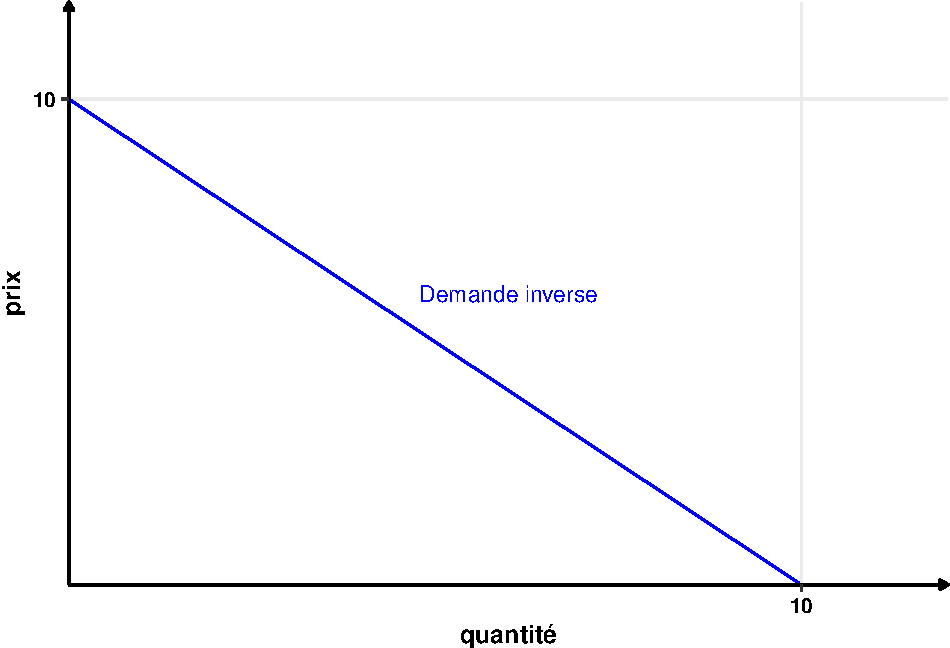
\includegraphics{_main_files/figure-latex/cppexo11-1.pdf}
\caption{\label{fig:cppexo11}Représentation graphique de la demande inverse.}
\end{figure}

\begin{enumerate}
\def\labelenumi{\arabic{enumi}.}
\setcounter{enumi}{1}
\item
  Pour la première unité de bien, on utilise la fonction de demande inverse.
  Le prix que le consommateur est prêt à payer pour la première unité est \(P(q=1)=9\).
  Pour la cinquième unité, c'est \(P(q=5)=5\).
  Dans les deux cas, ce sont le prix maximal que les consommateurs sont prêts à payer pour l'unité supplémentaire du bien.
  Rappelez-vous que la courbe de demande inverse représente l'ensemble des prix maximaux que les consommateurs sont prêts à payer pour une unité supplémentaire du bien.
\item
  Le surplus du consommateur est la somme des différences entre le prix maximal que chaque individu est prêt à payer et le prix auquel il paie effectivement le bien.
  Mathématiquement, le surplus du consommateur s'exprime toujours ainsi :
  \[
  S_c=\int_0^{q^*}P(q)-p^*dq
  \]
  Où \(p^*\) et \(q^*\) représente le prix sur le marché, et \(q^*\) la quantité échangée.
\end{enumerate}

\begin{figure}
\centering
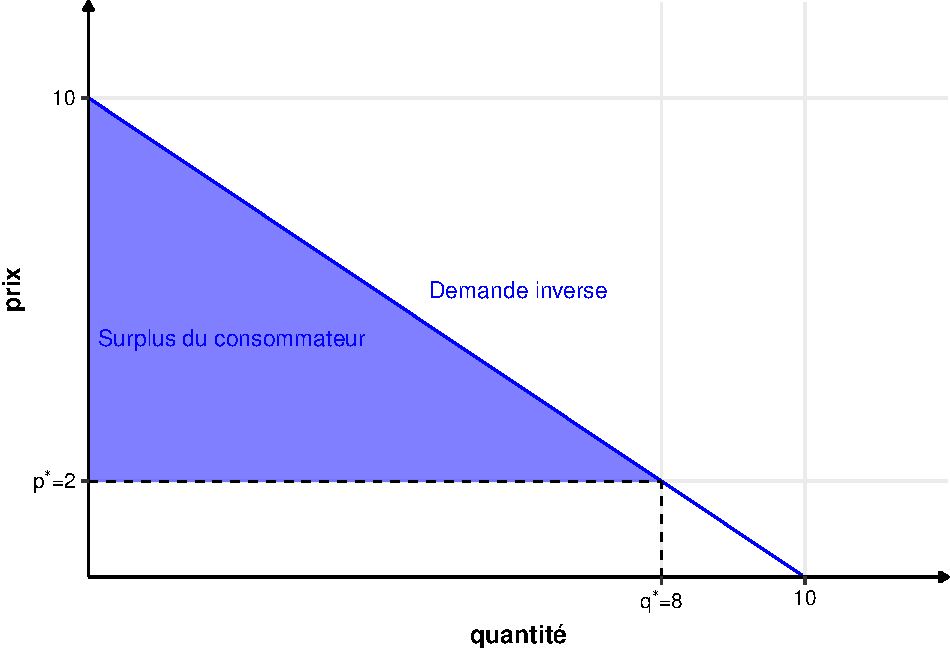
\includegraphics{_main_files/figure-latex/cppexo13-1.pdf}
\caption{\label{fig:cppexo13}Représentation graphique du surplus du consommateur.}
\end{figure}

En général, comme on peut le voir sur la figure \ref{fig:cppexo13}, il est possible de calculer le surplus en utiliser la formule donnant l'aire d'un triangle.
Ici, on obtient :
\[S_c=\frac{1}{2}(10-2)\cdot(8-0)=32\]
Les consommateurs ``gagnent'' donc 32 par rapport à la situation où ils devraient payer chacun leur prix de réserve.
\end{solution}

\begin{exercise}
\protect\hypertarget{exr:cppexo2}{}\label{exr:cppexo2}

On considère une firme faisant face à la contrainte technologique donnée par la fonction de coût total :
\[C(q)=q^2+10q\]

\begin{enumerate}
\def\labelenumi{\arabic{enumi}.}
\tightlist
\item
  Donnez la fonction de coût marginal correspondant.
\item
  Déterminez la fonction d'offre de cette firme. Représentez la graphiquement.
\item
  On suppose que la fonction de demande inverse du marché est donnée par :
  \[P(q)=100-q\]
  Déterminez le prix d'équilibre sur le marché, le surplus du producteur, le surplus du consommateur ainsi que le surplus total.
\item
  Supposons que l'État impose un prix \(p=80\). Quelle va être la quantité échangée ? Quel sera le surplus total ? Et si l'état impose un prix \(p=20\) ? Représentez graphiquement ces deux situations. En déduire que l'équilibre concurrentiel maximise le surplus total.
\end{enumerate}

\end{exercise}

\begin{solution}[Exercice \ref{exr:cppexo2}]
La fonction de coût marginal est la dérivée de la fonction de coût total.
La fonction de coût marginal donne le coût de production d'une unité de bien supplémentaire.
\[C_m(q)=C'(q)=2q+10\]

\begin{enumerate}
\def\labelenumi{\arabic{enumi}.}
\setcounter{enumi}{1}
\tightlist
\item
  La fonction d'offre des producteurs en concurrence pure et parfaite est égale à la fonction de coût marginal.
  Si on la note \(S\), \(S(q)=C_m(q) = 2q+10\).
  C'est le prix minimal auquel elle est prête à vendre une unité de bien supplémentaire.
\end{enumerate}

\begin{figure}
\centering
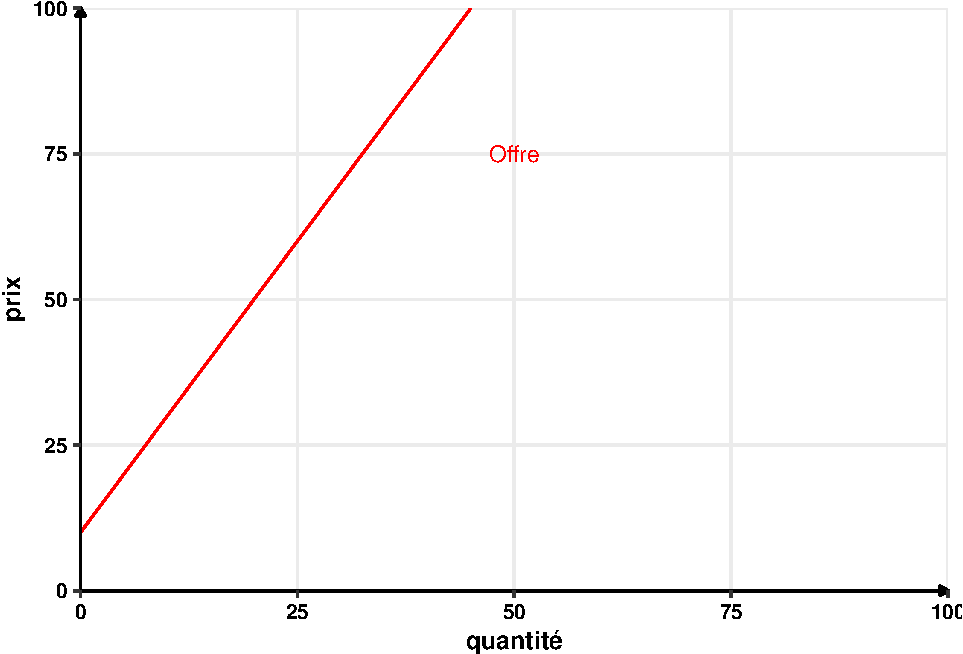
\includegraphics{_main_files/figure-latex/cppexo22-1.pdf}
\caption{\label{fig:cppexo22}Représentation graphique de la fonction d'offre.}
\end{figure}

\begin{enumerate}
\def\labelenumi{\arabic{enumi}.}
\setcounter{enumi}{2}
\tightlist
\item
  A l'équilibre sur le marché, une quantité \(q^*\) de biens est échangée au prix \(p^*\).
  Le marché vérifie alors les équations suivantes :
  \begin{equation}
  p^*=S(q^*)=P(q^*)
  \label{eq:cppequilibre}
  \end{equation}
  Commençons par la deuxième partie de l'équation \eqref{eq:cppequilibre} :
  \[
  \begin{array}{crcl}
  &2q^*+10&=&100-q^*\\
  \Leftrightarrow&3q^*&=&90\\
  \Leftrightarrow & q^*&=&30
  \end{array}
  \]
  La quantité échangée à l'équilibre est donc de \(q^*=30\).
  A l'aide de la quantité échangée est de la première partie de l'équation \eqref{eq:cppequilibre}, on obtient
  \[
  p^*=P(q^*=30) = 100-30=70 
  \]
  Sur le marché, 30 unités de bien sont donc échangés au prix de 70.
  On peut alors représenter les surplus sur le marché, comme dans la figure \ref{fig:cppexo23}.
  Le surplus des consommateurs est l'aire du triangle bleu, il vaut
  \[S_c=\frac{1}{2}(100-70)\times(30-0)=450\]
  Le surplus des producteurs est l'aire du triangle rouge :
  \[
  S_p=\frac{1}{2}(70-10)\times(30-0) = 900
  \]
\end{enumerate}

\begin{figure}
\centering
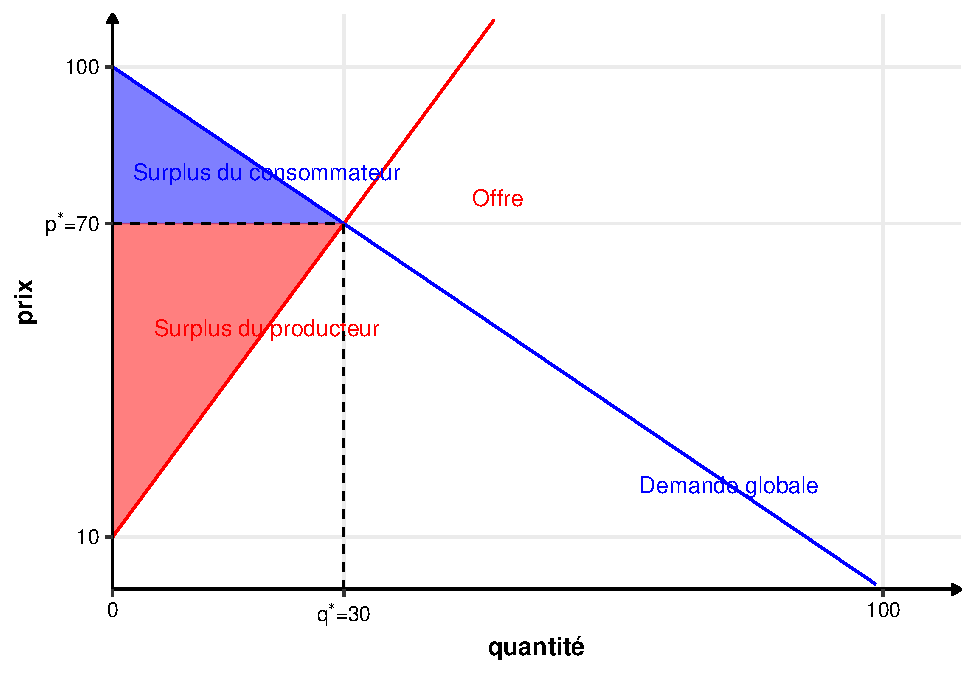
\includegraphics{_main_files/figure-latex/cppexo23-1.pdf}
\caption{\label{fig:cppexo23}Surplus en CPP.}
\end{figure}

Le surplus total est la somme des surplus des producteurs et des consommateurs :
\[
S_t^{CPP}=S_c+S_p=1350
\]

\begin{enumerate}
\def\labelenumi{\arabic{enumi}.}
\setcounter{enumi}{3}
\tightlist
\item
  On regarde maintenant le cas l'état impose un prix \(p^E=80\).
  La demande globale vaut alors de \(Q(p^E)=100-p^E=20\), que l'on l'obtient en inversant la demande inverse, autrement dit en trouvant la quantité \(q\) telle que \(P(q)=p^E=80\).
  L'offre globale vaut \(S(p^E)=\frac{p^E-10}{2}=35\), que l'on obtient en inversant la fonction d'offre, autrement dit en trouvant la quantité \(q\) telle que \(S(q)=p^E=80\).
  La demande globale est plus faible que l'offre globale, c'est donc la demande globale qui fixera les quantités échangées.
  La quantité échangée vaut donc 20.
  Graphiquement, on obtient la figure \ref{fig:cppexo24prixhaut}.
\end{enumerate}

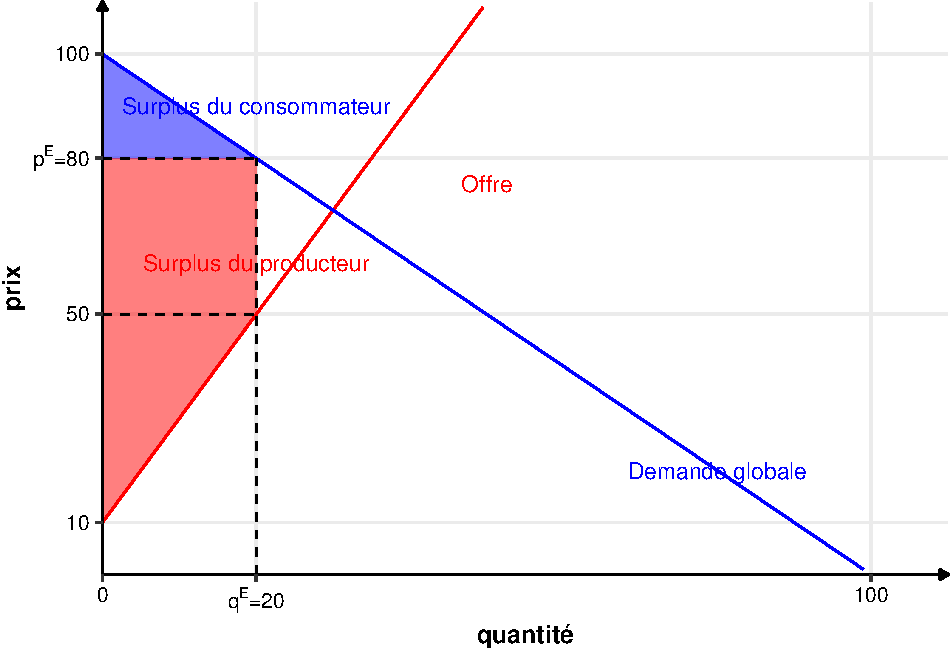
\includegraphics{_main_files/figure-latex/cppexo24prixhaut-1.pdf}
Le surplus total est dans ce cas l'aire du trapèze bleu et rouge.
Il nous faut obtenir le point sur la courbe d'offre pour la quantité \(q^E\).
En ce point, le prix est \(S(q^E)=50\).
\[
S_t=\frac{1}{2}(100-10+80-50)\times(20-0)=1200 < S_t^{CPP}
\]
Le surplus total est dans ce cas plus faible qu'en CPP.

On s'intéresse finalement au cas où l'état impose un prix \(p^E=20\).
La demande globale vaut alors de \(Q(p^E)=100-p^E=80\), que l'on l'obtient en inversant la demande inverse, autrement dit en trouvant la quantité \(q\) telle que \(P(q)=p^E=20\).
L'offre globale vaut \(S(p^E)=\frac{p^E-10}{2}=5\), que l'on obtient en inversant la fonction d'offre, autrement dit en trouvant la quantité \(q\) telle que \(S(q)=p^E=20\).
L'offre globale est plus faible que la demande globale, c'est donc l'offre globale qui fixera les quantités échangées.
La quantité échangée vaut donc 20.
Graphiquement, on obtient la figure \ref{fig:cppexo24prixbas}.

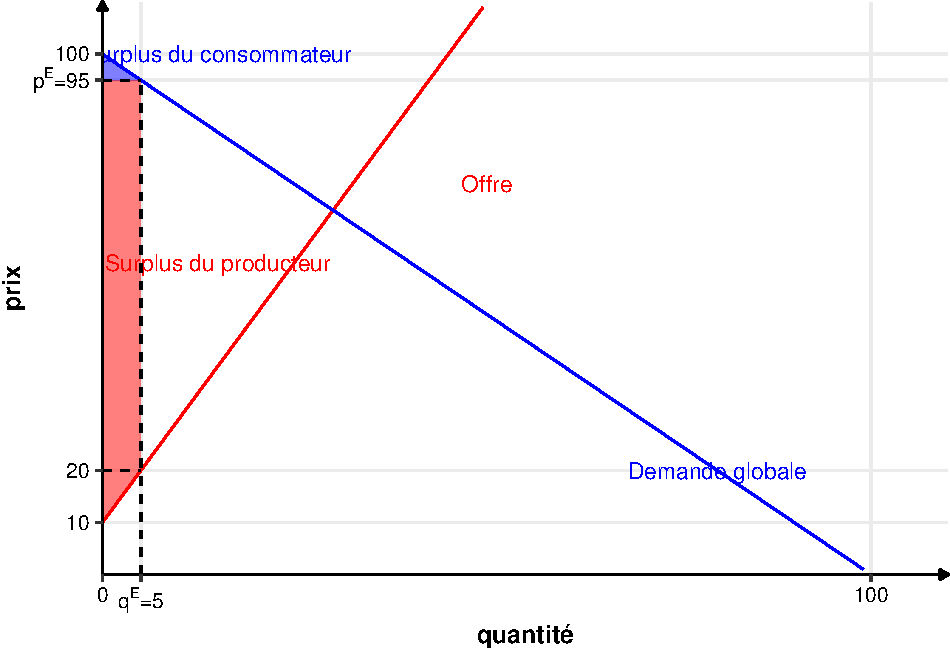
\includegraphics{_main_files/figure-latex/cppexo24prixbas-1.pdf}
Le surplus total est dans ce cas l'aire du trapèze bleu et rouge.
Il nous faut obtenir le point sur la courbe d'offre pour la quantité \(q^E\).
En ce point, le prix est \(S(q^E)=20\).
\[
S_t=\frac{1}{2}(100-10+95-20)\times(5-0)=\frac{825}{2}=412.5 < S_t^{CPP}
\]
Le surplus total est dans ce cas aussi plus faible qu'en CPP.

Ces deux situations illustrent les deux cas qui s'écartent de la CPP : un prix plus élevé ou un prix plus faible.
Dans les deux cas, on voit que le surplus total est plus faible.
Ce serait vrai pour n'importe quel prix différent du prix de la concurrence pure et parfaite.
On illustre ainsi le fait que l'équilibre de CPP maximise le surplus total.
\end{solution}

\hypertarget{exercices-sur-le-comportement-monopole}{%
\section{Exercices sur le comportement monopole}\label{exercices-sur-le-comportement-monopole}}

\begin{exercise}[Questions de cours]
\protect\hypertarget{exr:monoexo1}{}\label{exr:monoexo1}

Questions de cours :

\begin{enumerate}
\def\labelenumi{\arabic{enumi}.}
\tightlist
\item
  Quand la demande de bien est inélastique, la recette
  marginale est-elle positive ?
\item
  Un monopole maximise son profit dans la zone où les
  quantités demandées sont élastiques au prix. Vrai ou faux ?
\item
  Dans quel cas un monopole se comportera-t-il comme
  s'il était en situation de concurrence pure et parfaite (sans
  intervention de l'État) ?
\item
  Une entreprise a un taux de marge (indice de Lerner) de 45\%.
  Quelle est l'élasticité de la demande à laquelle
  elle fait face ?
\end{enumerate}

\end{exercise}

\begin{solution}[Solution de l'exercice \ref{exr:monoexo1}]

Réponses :

\begin{enumerate}
\def\labelenumi{\arabic{enumi}.}
\tightlist
\item
  Non, cf cours.
\item
  Vrai, cf cours.
\item
  Si l'élasticité prix de la demande est infini.
\item
  On a d'après la définition de l'indice de Lerner \eqref{eq:Lerner} :
  \[L=\frac{P(q^*)-C_m(q^*)}{P(q^*)}=\frac{1}{\left|\varepsilon_{p/q}(q^*)\right|}=0.45\]
  Donc \(\left|\varepsilon_{p/q}(q^*)\right| =1/0.45=20/9\).
\end{enumerate}

\end{solution}

\begin{exercise}
\protect\hypertarget{exr:monoexo2}{}\label{exr:monoexo2}

On considère une entreprise en monopole sur son marché dont la fonction de coût est :
\[C(q)=\frac{1}{20} q^2+15q+500\]
et qui fait face à la fonction de demande inverse : \[P(q)=45-0,2q\]

\begin{enumerate}
\def\labelenumi{\arabic{enumi}.}
\tightlist
\item
  Déterminer le prix \(p_m^*\) et la quantité \(q_m^*\) d'équilibre du monopole.
\item
  Les représenter graphiquement.
\item
  Calculer l'élasticité prix de la demande au point d'équilibre. Interpréter le résultat.
\item
  Calculer le surplus des consommateurs et le profit du monopole.
\item
  Déterminer le prix et la quantité correspondant à l'optimum de Pareto (concurrence pure et parfaite). Montrer que dans cette situation le surplus des consommateurs et le surplus social sont plus élevés, et que le profit du producteur est plus faible.
\item
  Calculer la charge morte du monopole.
\end{enumerate}

\end{exercise}

\begin{solution}[Solution de l'exercice \ref{exr:monoexo2}]

Réponses.

\begin{enumerate}
\def\labelenumi{\arabic{enumi}.}
\tightlist
\item
  À l'optimum, un monopole choisit la quantité telle que son coût marginal est égale à son revenu marginal :
  \[R_m(q^*)=C_m(q^*)\]
  Ici, on a :
  \[C_m(q^*)=\frac{1}{10}q+15\]
  Et :
  \[R(q) =qP(q)=45q-\frac{1}{5}q^2\]
  Donc :
  \[R_m(q)=45-\frac{2}{5}q\]
  À l'optimum, on doit donc avoir :
  \[
  \begin{array}{crcl}
  &45-\frac{2}{5}q^*&=&\frac{1}{10}q^*+15\\
  \Leftrightarrow & 30&=&\frac{1}{2}q^*\\
  \Leftrightarrow & q^*&=&60
  \end{array}
  \]
  On vérifie aussi la condition de second ordre \eqref{eq:cso} :
  \[R_m'(q^*)<C_m'(q^*)\]
  \[R'_m(q)=-\frac{2}{5}\]
  \[C'_m(q)=\frac{1}{10}>R_m'(q)\]
  La condition du second est bien vérifiée, nous avons bien un maximum ici.
  Finalement, le prix est \(p^*=P(q^*)=33\).
\end{enumerate}

\begin{figure}
\centering
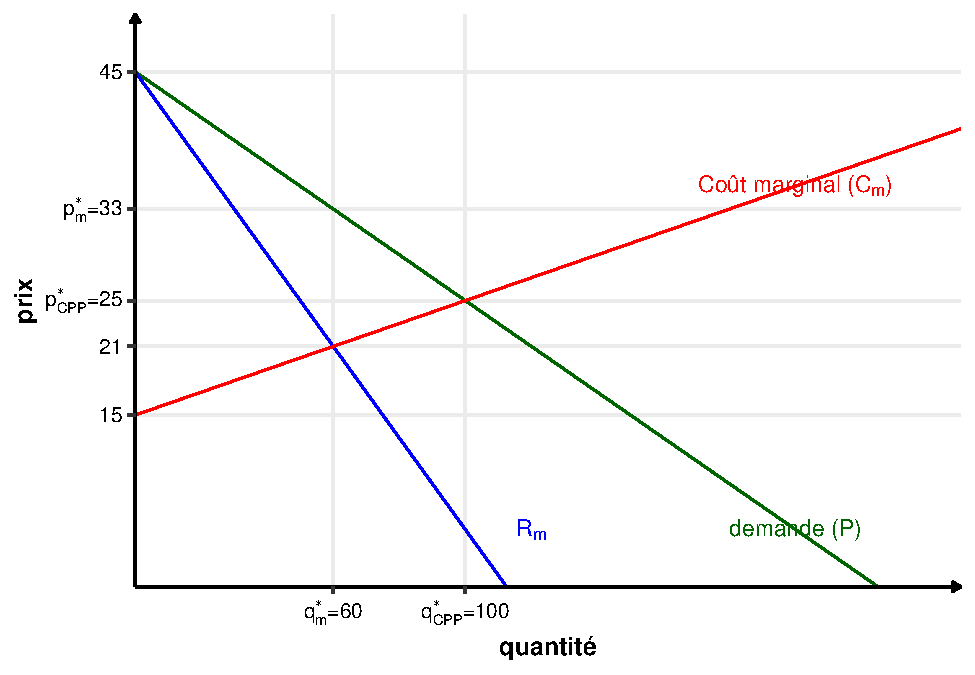
\includegraphics{_main_files/figure-latex/monoexo21-1.pdf}
\caption{\label{fig:monoexo21}Représentation graphique}
\end{figure}

\begin{enumerate}
\def\labelenumi{\arabic{enumi}.}
\setcounter{enumi}{2}
\item
  On a l'élasticité prix de la demande à l'équilibre :
  \[\varepsilon_{q/p}(q^*)=\frac{p^*}{q^*}\frac{1}{P'(q^*)}=\frac{33}{60}\frac{1}{-0.2}=-\frac{11}{4}\]
  La valeur absolue est bien plus grande que 1, nous sommes bien dans la zone où la demande est élastique.
  On peut aussi la calculer à l'aide de :
  \[\frac{p^*-C_m(q^*)}{p^*}=\frac{33-6-15}{33}=\frac{4}{11}=\frac{1}{|\varepsilon_{q/p}(q^*)|}\]
  On calcule ainsi le pouvoir du monopole : sa capacité à imposer au consommateur un prix à l'équilibre supérieur à son coût marginal.
\item
  Commençons par la représentation graphique.
\end{enumerate}

\begin{figure}
\centering
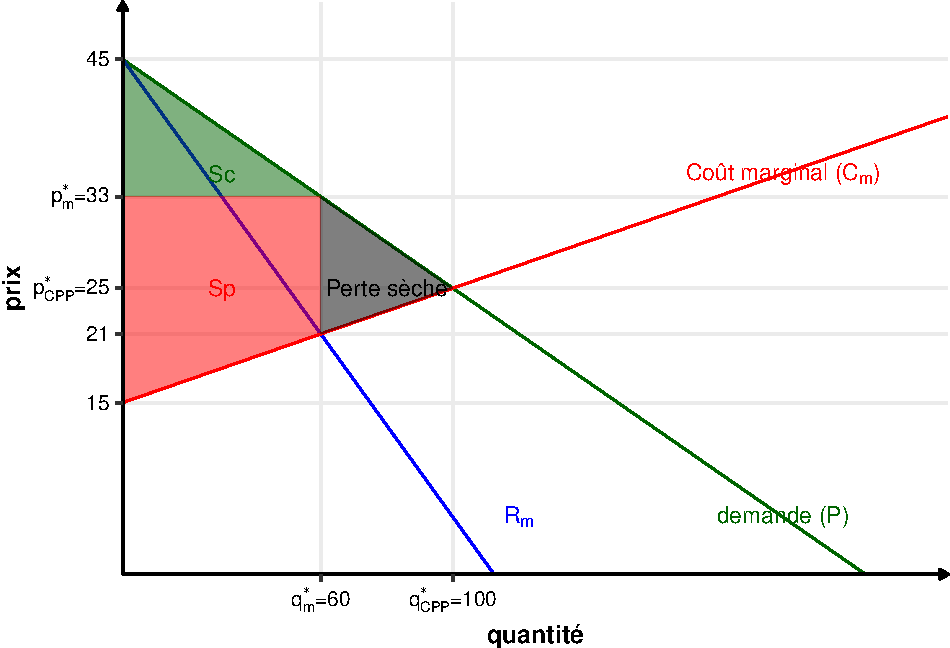
\includegraphics{_main_files/figure-latex/monoexo22-1.pdf}
\caption{\label{fig:monoexo22}Avec les surplus en monopole.}
\end{figure}

Le surplus des consommateurs se calcule en calculant l'aire du triangle vert dans la figure \ref{fig:monoexo22}.
On obtient :
\[S_c=\frac{(45-33)(60-0)}{2}=360\]
Le surplus du producteur s'obtient en calculant l'aire du trapèze rouge :
\[S_p=\frac{(33-15+33-21)(60-0)}{2}=900\]
Le profit du producteur est le surplus diminué du coût fixe, qui vaut ici 500. Le profit vaut donc 400.
Le surplus total est la somme des surplus des consommateurs et du producteur, soit \(S_T=1260\).

\begin{enumerate}
\def\labelenumi{\arabic{enumi}.}
\setcounter{enumi}{4}
\tightlist
\item
  En CPP, le prix est fixé par le marché et le prix est égal au coût marginal.
  On a (ici \(q^*\) et \(p^*\) sont différents des parties précédentes) :
  \[C_m(q^*)=P(q^*)=p^*\]
  Soit :
  \[\frac{1}{10}q^*+15=45-\frac{1}{5}q^*\]
  En résolvant l'équation, on obtient \(q^*=100\) et on peut en déduire \(p^*=25\).
  Pour calculer les surplus, on commence par la représentation graphique.
\end{enumerate}

\begin{figure}
\centering
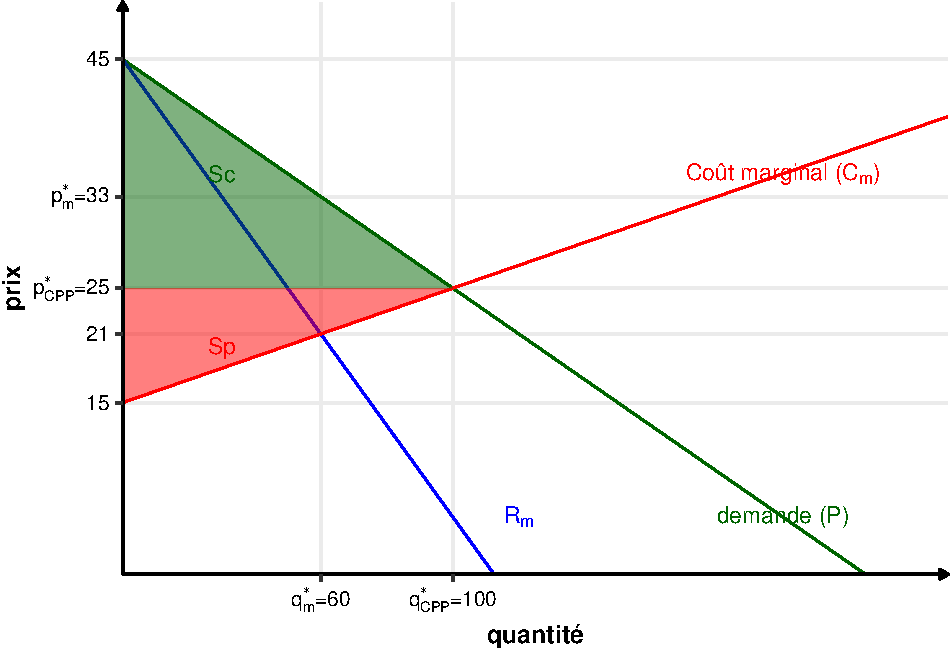
\includegraphics{_main_files/figure-latex/monoexo23-1.pdf}
\caption{\label{fig:monoexo23}Avec les surplus en CPP.}
\end{figure}

On calcule l'aire du triangle vert pour obtenir le surplus total des consommateurs.
Il vaut 1000, ce qui est supérieur au surplus obtenu en monopole.

On calcule l'aire du triangle rouge pour obtenir le surplus total du producteur.
Il vaut 500.
Si maintenant on enlève le coût fixe pour obtenir le profit, on obtient un profit nul.
Il est donc plus faible qu'en monopole.

Le surplus total en CPP vaudrait donc 1500, ce qui est supérieur au surplus total obtenu en monopole.

\begin{enumerate}
\def\labelenumi{\arabic{enumi}.}
\setcounter{enumi}{5}
\tightlist
\item
  La charge morte du monopole est la différence entre le surplus total en CPP et en monopole, soit \(1500-1260=240\).
  On peut aussi la calculer en utilisant l'aire du triangle noir sur la figure \ref{fig:monoexo22}.
\end{enumerate}

\end{solution}

\begin{exercise}
\protect\hypertarget{exr:monoexo3}{}\label{exr:monoexo3}

Sur un marché dominé par un producteur unique, la fonction de demande inverse pour une quantité \(q\) de bien est :
\[P(q)=250-q\]
La fonction de coût total du monopole est :
\[C(q)=4q^2+10q+400\]

\begin{enumerate}
\def\labelenumi{\arabic{enumi}.}
\tightlist
\item
  Quelle est la production d'équilibre du monopole ? Quel est le
  prix de vente ainsi que le profit du producteur ?
\item
  Comparez la solution précédente avec l'équilibre qui serait
  réalisé si l'entreprise se comportait comme en situation de
  concurrence pure et parfaite.
\item
  Dans chacun des cas ci-dessus, calculez le surplus du
  producteur, du consommateur, ainsi que le surplus total. Concluez
  sur l'impact de la présence d'un monopole sur le niveau de bien-être
  social.
\item
  Supposez que le producteur détienne un stock très important du bien
  (son coût marginal de production est nul). Donnez la solution du
  monopole dans une telle situation.
\end{enumerate}

\end{exercise}

\begin{solution}[Solution de l'exercice  \ref{exr:monoexo3}.]

Réponses:

\begin{enumerate}
\def\labelenumi{\arabic{enumi}.}
\tightlist
\item
  À l'optimum, un monopole choisit la quantité telle que son coût marginal est égale à son revenu marginal :
  \[R_m(q^*)=C_m(q^*)\]
  Ici, on a :
  \[C_m(q^*)=C'(q)=8q+10\]
  Et :
  \[R(q) =qP(q)=250q-q^2\]
  Donc :
  \[R_m(q)=R'(q)=250-2q\]
  À l'optimum, on doit donc avoir :
  \[
  \begin{array}{crcl}
  &250-2q^*&=&8q^*+10\\
  \Leftrightarrow & 240&=&10q^*\\
  \Leftrightarrow & q^*&=&24
  \end{array}
  \]
  On vérifie aussi la condition de second ordre \eqref{eq:cso} :
  \[R_m'(q^*)<C_m'(q^*)\]
  \[R'_m(q)=-2\]
  \[C'_m(q)=8>R_m'(q)\]
  La condition du second est bien vérifiée, nous avons bien un maximum ici.
  Le prix est \(p^*_M=P(q^*)=226\).
  Finalement, on peut calculer le profit :
  \[
  \pi^M(q^*)=R(q^*)-C(q^*)=p^*q^*-C(q^*)=24\times226-(4\times24^2+10\times24+400)=2480>0
  \]
  Le profit est bien positif, ce qui est la dernière condition à vérifier pour l'optimum.
\end{enumerate}

A l'optimum, il y a 24 unités de bien échangées sur le marché, au prix de 226.
Cela permet au monopole de faire un profit de 2480.

On représente graphiquement la situation obtenue sur la figure \ref{fig:monoexo31}.

\begin{enumerate}
\def\labelenumi{\arabic{enumi}.}
\setcounter{enumi}{1}
\tightlist
\item
  En CPP, le prix est fixé par le marché, le producteur le considère comme une donnée dans son optimisation.
  La courbe d'offre est égal à la courbe de coût marginal.
  À l'équilibre en CPP, l'offre est égale à la demande.
  On obtient (ici \(q^*\) et \(p^*\) sont différents des parties précédentes) :
  \[C_m(q^*)=P(q^*)=p^*\]
  Soit :
  \[8q^*+10=250-q^*\]
  En résolvant l'équation, on obtient \(q^*_{CPP}=80/3\) et on peut en déduire \(p^*_{CPP}=670/3\).
  On peut maintenant calculer le profit de la même manière que dans la question précédente, et on obtient \(\pi^{CPP}(q^*_{CPP})=22000/9<\pi^M\).
  Le profit du producteur en concurrence pure et parfaite est inférieur au profit en monopole.
  La quantité produite est supérieure et le prix du bien échangé inférieur.
\end{enumerate}

\begin{figure}
\centering
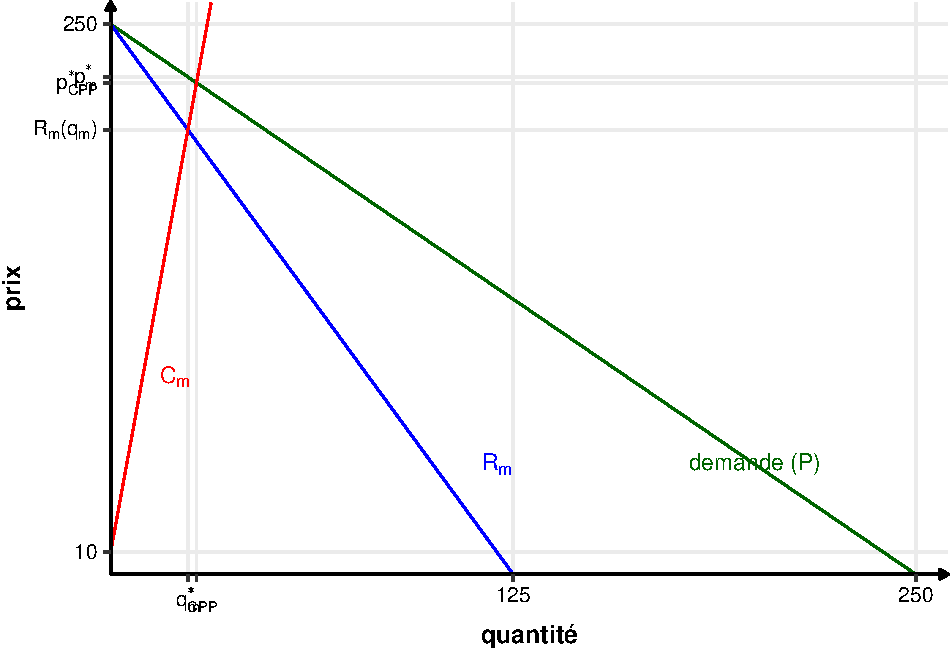
\includegraphics{_main_files/figure-latex/monoexo31-1.pdf}
\caption{\label{fig:monoexo31}Représentation graphique}
\end{figure}

\begin{enumerate}
\def\labelenumi{\arabic{enumi}.}
\setcounter{enumi}{2}
\tightlist
\item
  Pour calculer les surplus en monopole, commençons par la représentation graphique (figure \ref{fig:monoexo32}).
\end{enumerate}

\begin{figure}
\centering
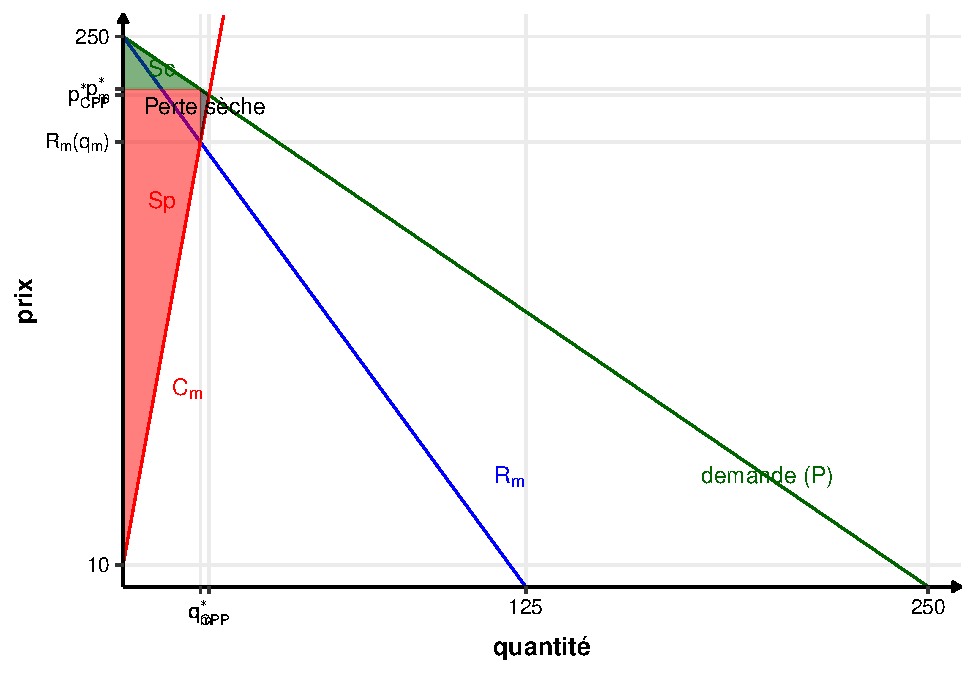
\includegraphics{_main_files/figure-latex/monoexo32-1.pdf}
\caption{\label{fig:monoexo32}Avec les surplus en monopole.}
\end{figure}

Le surplus des consommateurs se calcule en calculant l'aire du triangle vert dans la figure \ref{fig:monoexo32}.
On obtient :
\[S_c=\frac{(250-226)(24-0)}{2}=288\]
Le surplus du producteur s'obtient en calculant l'aire du trapèze rouge, ou bien en ajoutant le coût fixe (400 ici) au profit calculé à la question 1 :
\[S_p=\pi^M+CF=2480+400=2880\]
Le surplus total est la somme des surplus des consommateurs et du producteur, soit \(S_t^M=3168\).

Pour calculer les surplus en concurrence pure et parfaite, on commence par la représentation graphique (figure \ref{fig:monoexo33}).

\begin{figure}
\centering
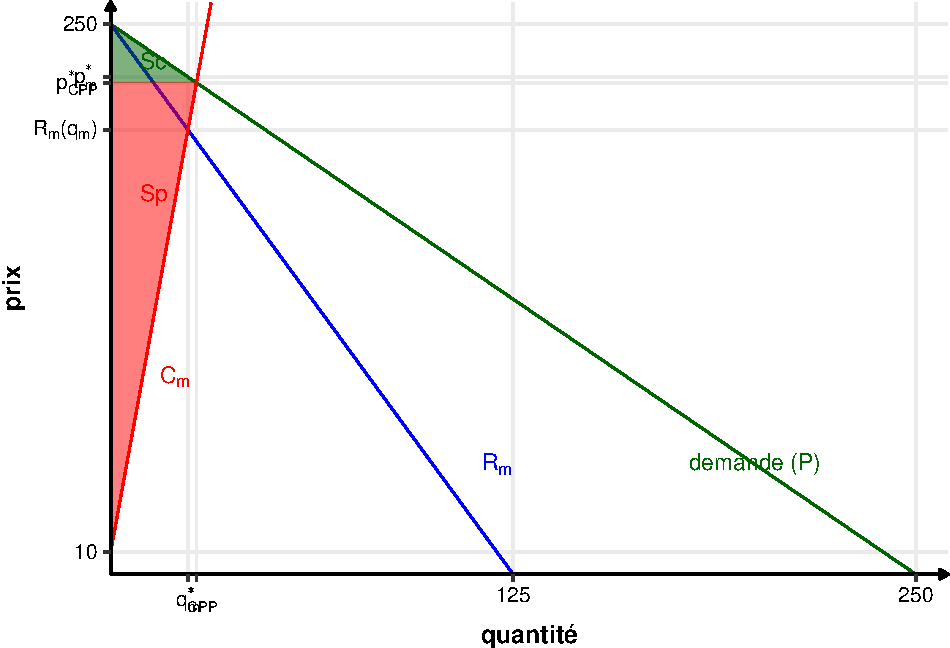
\includegraphics{_main_files/figure-latex/monoexo33-1.pdf}
\caption{\label{fig:monoexo33}Avec les surplus en CPP.}
\end{figure}

On calcule l'aire du triangle vert pour obtenir le surplus total des consommateurs.
Il vaut 3200/9, ce qui est supérieur au surplus obtenu en monopole.\\
On calcule l'aire du triangle rouge pour obtenir le surplus total du producteur, ou bien on ajoute le coût fixe (400 ici) au profit calculé à la question 2.
Il vaut ici 25600/9.
Il est donc plus faible qu'en monopole.\\
Le surplus total en CPP vaudrait donc 3200, ce qui est supérieur au surplus total obtenu en monopole.
Le monopole a un impact négatif sur le niveau de bien-être social.
Il introduit une charge morte de 32.

\begin{enumerate}
\def\labelenumi{\arabic{enumi}.}
\setcounter{enumi}{3}
\tightlist
\item
  À l'optimum, le monopole égalise recette marginale et coût marginal.
  Ici le coût marginal est nul, la recette marginale doit donc être nulle.
  On obtient donc l'équation :
  \[
  0=R_m(q^*)=250-2q^*
  \]
  On en déduit donc que \(q^*=125\).
  On peut alors calculer \(p^*=P(q^*)=125\).
  Quand le coût marginal du monopole est nul, il produit 125 unités de bien, vendues au prix 125.
\end{enumerate}

\end{solution}

\hypertarget{le-monopole-naturel-1}{%
\section{Le monopole naturel}\label{le-monopole-naturel-1}}

\begin{exercise}
\protect\hypertarget{exr:naturelexo1}{}\label{exr:naturelexo1}

On considère une entreprise en monopole sur son marché dont la fonction de coût est :
\[C(q)=\frac{5}{3}q^3-40q^2+340q\]
et qui fait face à la fonction de demande inverse :
\[P(q)=500-50q\]

\begin{enumerate}
\def\labelenumi{\arabic{enumi}.}
\tightlist
\item
  Calculer les grandeurs d'équilibre du monopole \((p^*_m,q^*_m)\).
\item
  Calculer le prix et la quantité d'équilibre de la concurrence pure et parfaite \((p^*_{cpp},q^*_{cpp}).\)
\item
  Calculer le profit du monopole dans ces deux situations. Interpréter le résultat.
\item
  Représenter graphiquement le coût marginal, le coût moyen, la demande et la recette marginale. Représenter la variation du profit du monopole entre ces deux situations.
\item
  Calculer le prix et la quantité assurant l'équilibre des finances du monopole, \((p_{B},q_{B})\). Comparer cette situation à l'optimum de Pareto de la concurrence pure et parfaite. Conclure.
\end{enumerate}

\end{exercise}

\begin{solution}[Solutions de l'exercice \ref{exr:naturelexo1}]

Réponses :

\begin{enumerate}
\def\labelenumi{\arabic{enumi}.}
\item
  À l'optimum, un monopole choisit la quantité telle que son coût marginal est égale à son revenu marginal :
  \[R_m(q^*)=C_m(q^*)\]
  Ici, on a :
  \[C_m(q^*)=C'(q)=5q^2-80q+340\]
  Et :
  \[R(q) =qP(q)=500q-50q^2\]
  Donc :
  \[R_m(q)=R'(q)=500-100q\]
  À l'optimum, on doit donc avoir :
  \[
  \begin{array}{crcl}
  &500-100q^*&=&5q^{*2}-80q^*+340\\
  \Leftrightarrow & 5q^{*2}+20q^*-160&=&0\\
  \Leftrightarrow & q^{*2}+4q^*-32&=&0
  \end{array}
  \]
  On doit donc résoudre une équation du second degré pour obtenir le résultat.
  On commence par calculer le discriminant :
  \[\Delta=b^2-4ac=4^2-4\times(-32)=16+128=144=12^2\]
  On en déduit que :
  \[q^8=\frac{-4\pm12}{2}=4\text{ ou } -8\]
  La solution \(q^*=-8\) est impossible, car les quantités sont forcément positives.
  La seule solution est donc \(q^*_m=4\).
  Remarquez qu'il est possible de ``voir'' sur l'équation du second degré que 4 était une racine et de se passer du calcul du discriminant.
  On vérifie aussi la condition de second ordre \eqref{eq:cso} :
  \[R_m'(q^*)<C_m'(q^*)\]
  \[R'_m(q)=-100\]
  \[C'_m(q)=10q-80\]
  En évaluant la dérivée du coût marginal en \(q^*\), on a \(C_m(q^*)=10\times4-80=-40>R_m(q^*)\)
  La condition du second est bien vérifiée, nous avons bien un maximum ici.
  Nous calculerons le profit à la question 3, nous n'allons donc pas le faire ici.
  Le prix est \(p^*_m=P(q^*_m)=300\).
\item
  En CPP, le prix est fixé par le marché, le producteur le considère comme une donnée dans son optimisation.
  La courbe d'offre est égal à la courbe de coût marginal.
  À l'équilibre en CPP, l'offre est égale à la demande.
  On obtient (ici \(q^*\) et \(p^*\) sont différents de la partie précédente) :
  \[C_m(q^*)=P(q^*)=p^*\]
  Soit :
  \[
  \begin{array}{crcl}
  &500-50q^*&=&5q^{*2}-80q^*+340\\
  \Leftrightarrow & 5q^{*2}-30q^*-160&=&0q^*\\
  \Leftrightarrow & q^{*2}-6q^*-32&=&0q^*
  \end{array}
  \]
  On doit donc résoudre une équation du second degré pour obtenir le résultat.
  On commence par calculer le discriminant :
  \[\Delta=(-6)^2+4\times32=36+128=164=4\times41\]
  On en déduit que :
  \[q^*=\frac{6\pm\sqrt{41}}{2}=3+\sqrt{41}\text{ ou } 3-\sqrt{41}\]
  La solution \(q^*=3-\sqrt{41}<0\) est impossible, car les quantités sont forcément positives.
  La seule solution est donc \(q^*_{CPP}=3+\sqrt{41}\approx\) 9.4.
  On peut en déduire \(p^*_{CPP}=50(7-\sqrt{41})\approx\) 29.84.
\item
  On calcule maintenant les profits.
  En monopole :
  \[\pi(p^*_m, q^*_m)=p^*_mq^*_m-C(q^*_m)=4\times300-\frac{5}{3}4^3+40\times4^2-340\times4=\frac{1120}{3}\approx 373,33\]
  En concurrence pure et parfaite :
  \[\pi(p^*_{CPP}, q^*_{CPP})=p^*_{CPP}q^*_{CPP}-C(q^*_{CPP})\approx-765\]
  Le profit des entreprises en concurrence pure et parfaite serait négatif.
  Le marché n'existerait donc pas, aucune entreprise ne souhaiterait produire pour faire des pertes.
  Cela signifie aussi qu'il ne serait pas possible pour l'État d'imposer au monopole une tarification au coût marginal.
  On est en fait dans une situation de monopole naturel, avec des coûts moyens décroissants.
  La tarification peut donc se faire au coût marginal, ce qu'on verra à la question 5.
\item
  Nous allons maintenant représenter graphiquement cette situation.
\end{enumerate}

\begin{figure}
\centering
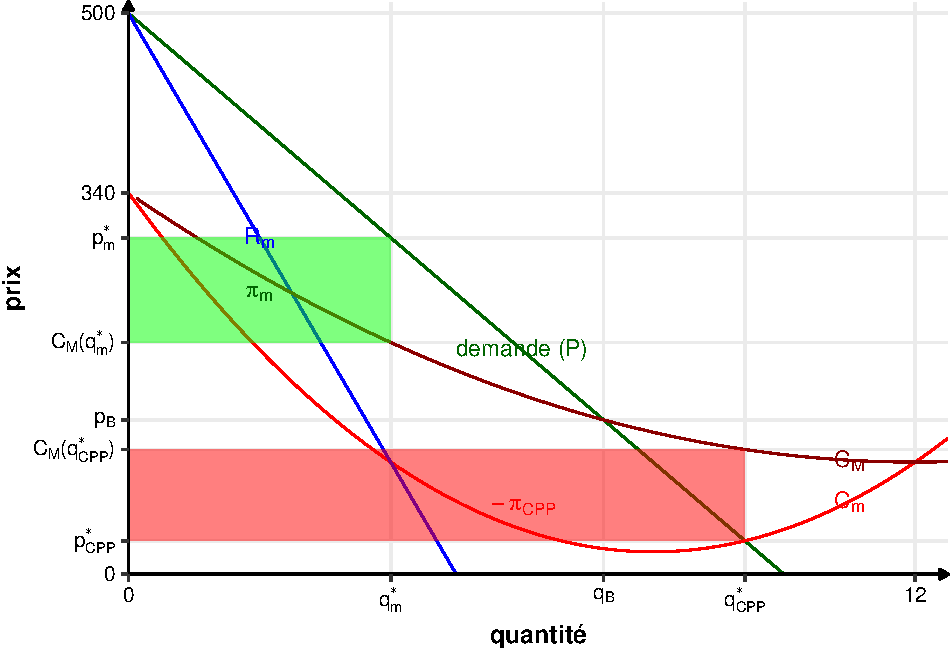
\includegraphics{_main_files/figure-latex/naturelexo1-1.pdf}
\caption{\label{fig:naturelexo1}Représentation graphique des équilibres}
\end{figure}

\begin{enumerate}
\def\labelenumi{\arabic{enumi}.}
\setcounter{enumi}{4}
\tightlist
\item
  Assurer l'équilibre des finances du monopole signifie faire en sorte qu'il ne fasse ni profits, ni pertes.
  Autrement dit, \(\pi(p_B, q_B)=0\).
  Cela se traduit par :
  \[
  \begin{array}{crcl}
  &p_Bq_B-C(q_B)&=&0 \\
  \Leftrightarrow & p_B&=&\frac{C(q_B)}{q_B}\\
  \Leftrightarrow & P(q_B)&=&C_M(q_B)
  \end{array}
  \]
  On oblige ainsi le monopole à fixer le prix à son coût moyen, ce qui est une manière de réguler un monopole naturel.
  On a \(C_M(q)=\frac{5}{3}q^2-40q+340\)
  On résout ainsi le problème :
  \[
  \begin{array}{crcl}
  &500-50q_B&=&\frac{5}{3}q_B^2-40q_B+340\\
  \Leftrightarrow & \frac{5}{3}q_B^2+10q_B-160&=&0\\
  \Leftrightarrow & q_B^2+6q_B-96&=&0
  \end{array}
  \]
  On doit donc résoudre une équation du second degré pour obtenir le résultat.
  On commence par calculer le discriminant :
  \[\Delta=6^2+4\times96=36+384=164=4\times105\]
  On en déduit que :
  \[q_B=\frac{-6\pm2\sqrt{105}}{2}=-3+\sqrt{105}\text{ ou } -3-\sqrt{105}\]
  La solution \(q_B=-3-\sqrt{105}<0\) est impossible, car les quantités sont forcément positives.
  La seule solution est donc \(q_{B}=-3+\sqrt{105}\approx\) 7.25.
  On peut en déduire \(p_{B}=50(13-\sqrt{105})\approx\) 137.65.\\
  On observe que \(p_B>p_{CPP}^*\) et \(q_B<q_{CPP}^*\), mais en échange, le monopole est à l'équilibre financier et produira.
  La situation n'est pas optimale au sens de Pareto, et il y aura une charge morte, mais l'optimum de Pareto est inatteignable sans subventionner le monopole.
  Il est impossible de le forcer à tarifer au coût marginal, en utilisant par exemple un prix maximal, car il ferait alors des pertes et ne produirait simplement pas.
  La solution de la tarification au cût moyen est en quelques sorte la deuxième meilleure solution possible, mais c'est la seule faisable.
\end{enumerate}

\end{solution}

\begin{exercise}
\protect\hypertarget{exr:naturelexo2}{}\label{exr:naturelexo2}

Un entreprise est en monopole sur un marché où la fonction de
demande est :
\[Q\left(p\right)=30-p\]
La fonction de coût total du monopole est :
\[C(q)=100+\frac{q^2}{2}\]

\begin{enumerate}
\def\labelenumi{\arabic{enumi}.}
\item
  Calculez le prix, la quantité d'équilibre et le profit. Représentez graphiquement cet équilibre et le surplus collectif.
\item
  L'État décide d'imposer au monopole une tarification au coût marginal. Expliquez cette décision. Représentez le nouvel équilibre et les surplus sur le précédent graphique. Commentez.
\item
  Calculez le surplus du consommateur et le surplus collectif sans et avec tarification au coût marginal.\\
  Après une innovation technologique, la fonction de coût devient :
  \[C(q)=100+\frac{q}{2}\]
\item
  L'État peut-il continuer à imposer une tarification au coût marginal ?
\item
  Quelle situation peut-il retenir ? Pourquoi ? Calculez et représentez le nouveau surplus collectif.
\end{enumerate}

\end{exercise}

\begin{solution}[Solution de l'exercice \ref{exr:naturelexo2}]

\begin{enumerate}
\def\labelenumi{\arabic{enumi}.}
\tightlist
\item
  À l'optimum, un monopole choisit la quantité telle que son coût marginal est égale à son revenu marginal :
  \[R_m(q^*)=C_m(q^*)\]
  Ici, on a :
  \[C_m(q^*)=C'(q)=q\]
  Et :
  \[R(q) =qP(q)=30q-q^2\]
  La fonction qui nous est donnée est la demande \(Q\) et non la demande inverse \(P\).
  On doit donc trouver la demande inverse, c'est à dire la fonction \(P\) telle que \(Q(P(q))=q\) :
  \[30-P(q)=q \Leftrightarrow P(q) = 30-q\]
  La fonction de demande inverse \(P\) est donc \(P(q)=30-q\).
  Donc :
  \[R_m(q)=R'(q)=30-2q\]
  À l'optimum, on doit donc avoir :
  \[
  \begin{array}{crcl}
  &30-2q^*&=&q^*\\
  \Leftrightarrow & q^*&=&10
  \end{array}
  \]
  On vérifie aussi la condition de second ordre \eqref{eq:cso} :
  \[R_m'(q^*)<C_m'(q^*)\]
  \[R'_m(q)=-2\]
  \[C'_m(q)=1>R_m'(q)\]
  La condition du second est bien vérifiée, nous avons bien un maximum ici.
  Le prix est \(p^*_m=P(q^*_m)=20\).
  Le profit est :
  \[\pi(q_m^*, p_m^*)=p_m^*q_m^*-C(q_m^*)=20\times10-\left(100+\frac{10^2}{2}\right)=50>0\]
  Le profit est bien positif.
  À l'optimum, 10 unités sont échangées sur ce marché, au prix de 20.
  Le monopole réalise alors un profit de 50.
\end{enumerate}

\begin{figure}
\centering
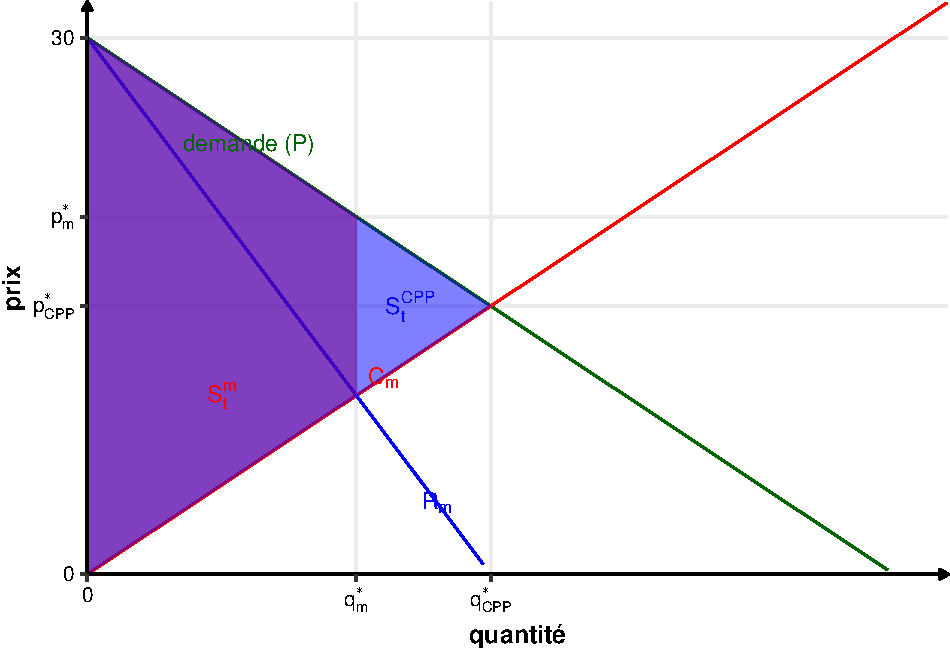
\includegraphics{_main_files/figure-latex/naturelexo21-1.pdf}
\caption{\label{fig:naturelexo21}Représentation graphique des équilibres}
\end{figure}

\begin{enumerate}
\def\labelenumi{\arabic{enumi}.}
\setcounter{enumi}{1}
\item
  La tarification au coût marginal du monopole a pour but d'obtenir l'équilibre de concurrence pure et parfaite, qui est un optimum de Pareto.
  L'État cherche en fait a augmenter le surplus collectif.
  Nous allons représenter ce nouvel équilibre comme étant l'équilibre de concurrence pure et parfaite.
\item
  Le surplus des consommateurs dans la situation de monopole (question 1) est donné par :
  \[S_c^m=\frac{1}{2}(30-p_m^*)\times q_m^*=\frac{1}{2}(30-20)\times 10=50\]
  Le surplus du monopole est donné par :
  \[S_p^m=\pi^m+CF=50+100=150\]
  Car le coût fixe vaut 50.
  Le surplus collectif est donc de :
  \[S_t^m=S_c^m+S_p^m=150+50=200\]
  Pour calculer les surplus avec la tarification au coût marginal, nous devons commencer par calculer les quantités et prix de l'échange.
  Nous avons l'équation suivante dans cette configuration :
  \[C_m(q^*)=P(q^*)=p^*\]
  Soit :
  \[q^*=30-q^*\Leftrightarrow q^*_{CPP}=15\]
  Et :
  \[p^*_{CPP}=P(q^*)=q^*=15\]
  En tarifiant au coût marginal, il y a donc 15 unités de biens échangées sur le marché, au prix de 15.
  Le surplus des consommateurs est alors :
  \[S_c^{CPP}=\frac{1}{2}(30-p_{CPP}^*)\times q_{CPP}^*=\frac{1}{2}(30-15)\times 15=\frac{225}{2}>S_c^m\]
  Le surplus du producteur est :
  \[S_p^{CPP}=\frac{1}{2}(p_{CPP}^*-0)\times q_{CPP}^*=\frac{1}{2}(30-15)\times 15=\frac{225}{2}<S_p^m\]
  On en déduit que le surplus total est :
  \[S_t^{CPP}=S_c^{CPP}+S_p^{CPP}=\frac{225}{2}+\frac{225}{2}=225>S_t^m\]
  Le surplus collectif est plus important quand l'Etat impose une tarification au coût marginal que quand il le laisse choisir sa quantité ou son prix.
\item
  Avec cette nouvelle fonction de coût, le coût marginal devient :
  \[C_m(q)=\frac{1}{2}\]
  La tarification au coût marginal donnerait donc un prix de l'échange de \(p^*=1/2\).
  On peut calculer le coût moyen d'une unité produite :
  \[C_M(q)=\frac{C(q)}{q}=\frac{100}{q}+\frac{1}{2}>\frac{1}{2}=p^*\]
  Le coût moyen d'une unité produite serait donc supérieur au prix de l'échange, et ce, quelque soit le nombre d'unités produites.
  Le producteur ferait donc systématiquement des pertes, à cause de ces coûts fixes, ce qui n'est pas une situation soutenable.
  Il se retirerait donc du marché.
\end{enumerate}

Rappel : \(\pi(q)=pq-C(q)=q(p-C(q)/q)=q(p-C_M(q))\).

\begin{enumerate}
\def\labelenumi{\arabic{enumi}.}
\setcounter{enumi}{4}
\tightlist
\item
  L'Etat peut forcer le monopole à tarifer au coût moyen et à répondre à toute la demande.
  En l'obligeant à vendre à son coût moyen de production, il s'assure que le monopole ne fait ni bénéfices, ni pertes.
  On a alors la condition d'équilibre :
  \[C_M(q^*)=P(q^*)=p^*\]
  On résout l'équation de gauche :
  \[
  \begin{array}{crcl}
  &C_M(q^*)&=&P(q^*)\\
  \Leftrightarrow&\frac{100}{q^*}+\frac{1}{2}&=&30-q^*\\
  \Leftrightarrow&200+q^*&=&60q^*-2q^{*2}\\
  \Leftrightarrow&2q^{*2}-59q^*+200&=&0\\
  \end{array}
  \]
  Pour trouver la solution, on doit donc résoudre une équation du second degré.
  On commence par calculer le discriminant :
  \[\Delta=(-59)^2-4\times200\times2=3481-1600=1881=9\times209\]
  On en déduit que :
  \[q^*=\frac{59\pm3\sqrt{209}}{4}\]
  Les deux racines sont positives, l'obligation de satisfaire toute la demande font que l'on prend la racine la plus grande.
  La solution est donc \(q^*=\frac{59+3\sqrt{209}}{4}\approx\) 25.59.
  On peut en déduire \(p^*=\frac{61-3\sqrt{209}}{4}\approx\) 4.41.
\end{enumerate}

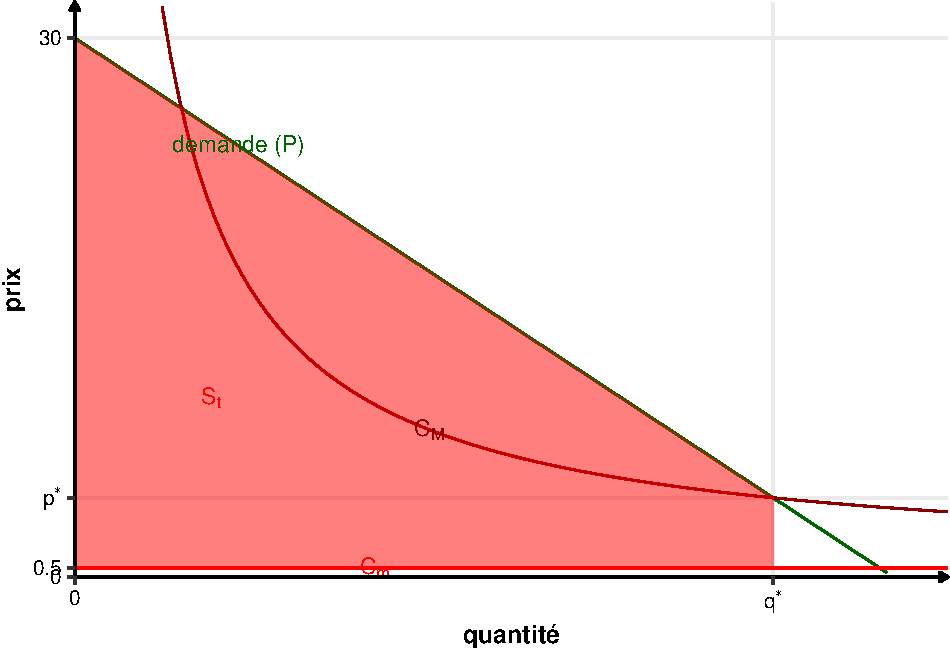
\includegraphics{_main_files/figure-latex/naturelexo25-1.pdf}
On représente graphiquement le surplus collectif sur la figure \ref{fig:naturelexo25}.
On voit que le surplus collectif est un trapèze : \[S_t=\left(30−\frac{1}{2}+p^*−\frac{1}{2}\right)×\frac{q^*}{2}=(29−p^*)\times \frac{q^*}{2}\]
En calculant (à la calculatrice), on obtient \(S_t\approx\) 314.69.

\end{solution}

\begin{exercise}
\protect\hypertarget{exr:naturelexo3}{}\label{exr:naturelexo3}

La demande d'un bien est donnée par : \[Q\left(p\right)=1000-50p\] Le coût
marginal et le coût moyen sont fixes à 10€ l'unité.

\begin{enumerate}
\def\labelenumi{\arabic{enumi}.}
\tightlist
\item
  Quels sont les prix et les quantités d'équilibre en concurrence
  et en monopole ?
\item
  L'État impose une taxe de 2 euros par unité. Quels sont les nouveaux prix et quantités en concurrence et en monopole ?
\item
  Quelle est la part de l'augmentation des prix supportée par les consommateurs en monopole et en concurrence ?
\end{enumerate}

\end{exercise}

\begin{solution}[Solution de l'exercice \ref{exr:naturelexo2}]
En lisant les données, nous pouvons écrire les fonctions de coût marginal et de coût moyen :
\[C_m(q)=10\qquad C_M(q)=10\]
On peut en déduire que la fonction de coût total est \(C(q)=10q\).\\
La fonction qui nous est donnée est la demande \(Q\) et non la demande inverse \(P\).
Pour résoudre l'exercice, nous avons besoin de la fonction de demande inverse, c'est à dire la fonction \(P\) telle que \(Q(P(q))=q\) :
\[1000-50P(q)=q \Leftrightarrow P(q) = 20-\frac{q}{50}\]

\begin{enumerate}
\def\labelenumi{\arabic{enumi}.}
\tightlist
\item
  Nous allons commencer par résoudre le problème du monopole.
  À l'optimum, un monopole choisit la quantité telle que son coût marginal est égale à son revenu marginal :
  \[R_m(q^*)=C_m(q^*)\]
  Ici, on a :
  \[R(q) =qP(q)=20q-\frac{1}{50}q^2\]
  Donc :
  \[R_m(q)=R'(q)=20-\frac{1}{25}q\]
  À l'optimum, on doit donc avoir :
  \[
  \begin{array}{crcl}
  &20-\frac{1}{25}q^*_m&=&10\\
  \Leftrightarrow & q^*_m&=&250
  \end{array}
  \]
  On vérifie aussi la condition de second ordre \eqref{eq:cso} :
  \[R_m'(q^*)<C_m'(q^*)\]
  \[R'_m(q)=-1/25\]
  \[C'_m(q)=10>R_m'(q)\]
  La condition du second est bien vérifiée, nous avons bien un maximum ici.
  Le prix est \(p^*_m=P(q^*_m)=15>10=C_M(q)\).
  Le prix est supérieur au coût moyen, donc les profits seront positifs.
  À l'optimum, 250 unités sont échangées sur ce marché, au prix de 15€.\\
  Résolvons maintenant le problème en concurrence pure et parfaite.
  La condition d'équilibre en concurrence pure et parfaite est :
  \[C_m(q^*)=P(q^*)=p^*\]
  Soit :
  \[10=20-\frac{1}{50}q^*_{CPP}\Leftrightarrow q^*_{CPP}=500>q_m^*\]
  Et :
  \[p^*_{CPP}=P(q^*)=10<p_m^*\]
  En concurrence pure et parfaite, 500 unités de biens sont échangées sur le marché à un prix de 10€.
  Les quantités échangées sont plus importantes et le prix plus faible qu'en monopole.\\
  \emph{Remarque :} On peut procéder à une résolution alternative en CPP, sans utiliser la demande inverse.
  On a en effet la condition d'équilibre du marché : \(C_m(q^*)=P(q^*)=p^*\).
  Ici, \(C_m(q^*)\) est constant et égal à 10, on a donc immédiatement \(p^*=C_m(q^*)=10\).
  On peut alors utiliser la fonction de demande \(Q\) : \(q^*=Q(p^*)=1000-50\times10=500\).
  On obtient bien les mêmes résultats qu'en utilisant la demande inverse.
  Dans cette exercice, on a néanmoins besoin de la demande inverse pour le monopole, s'en passer n'est donc pas possible.
\item
  L'imposition d'une taxe unitaire (une taxe sur chaque unité produite) revient à augmenter le coût marginal et le coût moyen du producteur de 2€.
  On a donc maintenant \(C_m(q)=C_M(q)=10+2=12\) (et \(C(q)=12q\)).
  On résout maintenant le problème comme précédemment.\\
  Nous allons commencer par résoudre le problème du monopole.
  À l'optimum, un monopole choisit la quantité telle que son coût marginal est égale à son revenu marginal :
  \[R_m(q^*)=C_m(q^*)\]
  Ici, on a :
  \[R(q) =qP(q)=20q-\frac{1}{50}q^2\]
  Donc :
  \[R_m(q)=R'(q)=20-\frac{1}{25}q\]
  À l'optimum, on doit donc avoir :
  \[
  \begin{array}{crcl}
  &20-\frac{1}{25}q^*_m&=&12\\
  \Leftrightarrow & q^*_m&=&200
  \end{array}
  \]
  On vérifie aussi la condition de second ordre \eqref{eq:cso} :
  \[R_m'(q^*)<C_m'(q^*)\]
  \[R'_m(q)=-1/25\]
  \[C'_m(q)=12>R_m'(q)\]
  La condition du second est bien vérifiée, nous avons bien un maximum ici.
  Le prix est \(p^*_m=P(q^*_m)=16>12=C_M(q)\).
  Le prix est supérieur au coût moyen, donc les profits seront positifs.
  À l'optimum, 200 unités sont échangées sur ce marché, au prix de 16€.\\
  Résolvons maintenant le problème en concurrence pure et parfaite.
  La condition d'équilibre en concurrence pure et parfaite est :
  \[C_m(q^*)=P(q^*)=p^*\]
  Soit :
  \[12=20-\frac{1}{50}q^*_{CPP}\Leftrightarrow q^*_{CPP}=400>q_m^*\]
  Et :
  \[p^*_{CPP}=P(q^*)=12<p_m^*\]
  En concurrence pure et parfaite, 400 unités de biens sont échangées sur le marché à un prix de 12€.
  Les quantités échangées sont plus importantes et le prix plus faible qu'en monopole.
\item
  En concurrence pure et parfaite, l'augmentation du prix lié à la taxe est entièrement supportée par les consommateurs, puisque le nouveau prix est supérieur de 2€ au précédent.
  En monopole, le nouveau prix est supérieur de 1€ au précédent.
  Les consommateurs absorbent donc la moitié de l'augmentation du prix, et le monopole en absorbe l'autre moitié.
\end{enumerate}

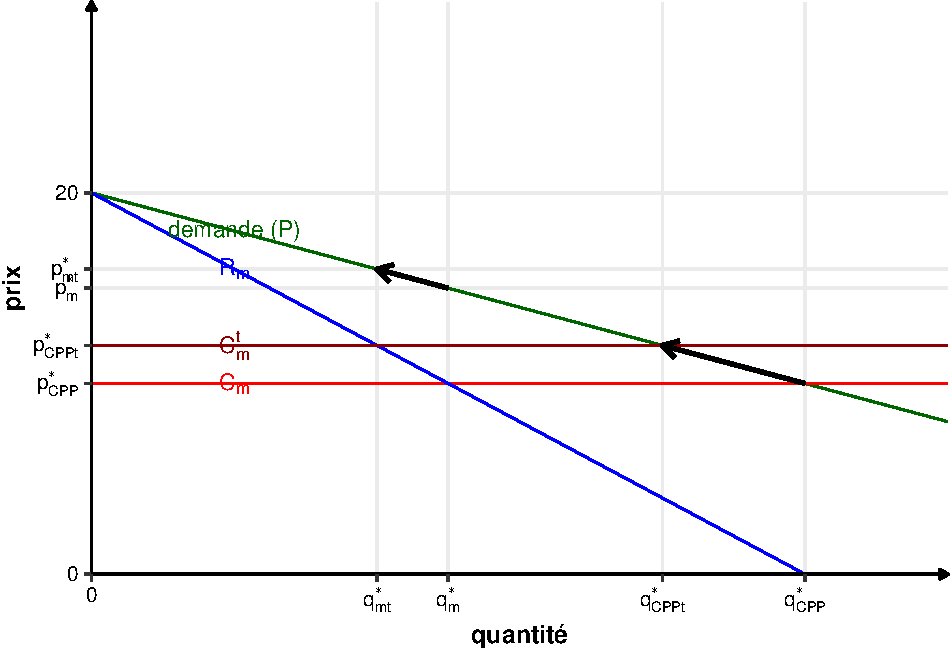
\includegraphics{_main_files/figure-latex/naturelexo3-1.pdf}
\end{solution}

\begin{exercise}
\protect\hypertarget{exr:naturelexo4}{}\label{exr:naturelexo4}

Une entreprise en monopole a une fonction de coût total de :
\[C(q)=3q^2\]
La fonction de demande sur son marché est :
\[P(q)=1200-q\]

\begin{enumerate}
\def\labelenumi{\arabic{enumi}.}
\tightlist
\item
  Donnez la quantité produite, le prix de vente ainsi que le
  profit à la solution du monopole.
\item
  Que fera l'entreprise si elle est confrontée à une taxe
  forfaitaire de 50 000€ ? Et si la taxe est de 100 000€ ?
\item
  L'État souhaite maximiser le surplus total en instaurant un
  prix plafond. À quel niveau doit-il le fixer ?
\item
  Que fera le monopole s'il doit payer une taxe de 40€
  par unité ? Quels seront alors ses profits ?
\end{enumerate}

\end{exercise}

\begin{solution}[Solutions de l'exercice \ref{exr:naturelexo4}]

Réponses

\begin{enumerate}
\def\labelenumi{\arabic{enumi}.}
\tightlist
\item
  À l'optimum, un monopole choisit la quantité telle que son coût marginal est égale à son revenu marginal :
  \[R_m(q^*)=C_m(q^*)\]
  Ici, on a :
  \[R(q) =qP(q)=1200q-q^2\]
  Et :
  \[C_m(q)=C'(q)=6q\]
  Donc :
  \[R_m(q)=R'(q)=1200-2q\]
  À l'optimum, on doit donc avoir :
  \[
  \begin{array}{crcl}
  &1200-2q^*_m&=&6q^*_m\\
  \Leftrightarrow & q^*_m&=&150
  \end{array}
  \]
  On vérifie aussi la condition de second ordre \eqref{eq:cso} :
  \[R_m'(q^*)<C_m'(q^*)\]
  \[R'_m(q)=-2\]
  \[C'_m(q)=6>R_m'(q)\]
  La condition du second est bien vérifiée, nous avons bien un maximum ici.
  Le prix est \(p^*_m=P(q^*_m)=1050\).
  On calcule le profit :
  \[\pi_m=p_m^*q_m^*-C(q^*_m)=1050\times150-3\times150^2=90000>0\]
  À l'optimum, 150 unités sont échangées sur ce marché, au prix de 1050€.
  Le monopole réalise alors un profit de 90 000€.
\item
  Une taxe forfaitaire ne change pas le comportement du monopole, sauf si la taxe forfaitaire transforme le profit du monopole en pertes.
  Le profit réalisé par le monopole devient avec la taxe forfaitaire \(T\) :
  \[\pi_m=p_m^*q_m^*-C(q^*_m)-T=1050\times150-3\times150^2-T=90000-T\]
  On en conclut que si la taxe forfaitaire est de 50 000€, le monopole continuera de produire normalement, mais si la taxe est de 100 000€, il arrêtera de produire et fermera.
\item
  L'Etat doit fixer un prix plafond qui est égal au prix de la concurrence pure et parfaite pour maximiser le surplus total.
  Cherchons donc l'équilibre de concurrence pure et parfaite.
  La condition d'équilibre en concurrence pure et parfaite est :
  \[C_m(q^*)=P(q^*)=p^* (=p_{max})\]
  Soit :
  \[6q^*_{CPP}=1200-q^*_{CPP}\Leftrightarrow q^*_{CPP}=\frac{1200}{7}>150=q_m^*\]
  Et :
  \[p_{max}=P(q^*)=\frac{7200}{7}<1050=p_m^*\]
  L'Etat doit donc fixer un prix plafond de \(\frac{7200}{7}\approx\) 3600€ pour maximiser le surplus total.
\item
  Une taxe unitaire de 40€ revient donc à augmenter le coût de production par unité de 40€ pour le monopole.
  Le coût marginal du monopole devient donc \(C_m(q)=6q+40\).
  À l'optimum, un monopole choisit la quantité telle que son coût marginal est égale à son revenu marginal :
  \[R_m(q^*)=C_m(q^*)\]
  Avec :
  \[R_m(q)=1200-2q\]
  À l'optimum, on doit donc avoir :
  \[
  \begin{array}{crcl}
  &1200-2q^*_m&=&6q^*_m+40\\
  \Leftrightarrow & q^*_m&=&145
  \end{array}
  \]
  On vérifie aussi la condition de second ordre \eqref{eq:cso} :
  \[R_m'(q^*)<C_m'(q^*)\]
  \[R'_m(q)=-2\]
  \[C'_m(q)=6>R_m'(q)\]
  La condition du second est bien vérifiée, nous avons bien un maximum ici.
  Le prix est \(p^*_m=P(q^*_m)=1055\).
  On calcule le profit :
  \[\pi_m=p_m^*q_m^*-C(q^*_m)=1055\times145-(3\times145^2+40\times 145)=84100>0\]
  À l'optimum avec une taxe unitaire de 40€, 145 unités sont échangées sur ce marché, au prix de 1055€.
  Le monopole réalise alors un profit de 84 100€.
  L'augmentation du prix est de 5€, cela signifie que 35€ de la taxe sera payée par le monopole.
  Nous sommes ici dans un cas où le monopole supportera l'essentiel du prix de la taxe.
\end{enumerate}

\end{solution}

\hypertarget{appendix-annexes}{%
\appendix}


\hypertarget{ruxe9solution-des-probluxe8mes}{%
\chapter{Résolution des problèmes}\label{ruxe9solution-des-probluxe8mes}}

\begin{longtable}[]{@{}
  >{\raggedright\arraybackslash}p{(\columnwidth - 4\tabcolsep) * \real{0.34}}
  >{\centering\arraybackslash}p{(\columnwidth - 4\tabcolsep) * \real{0.28}}
  >{\centering\arraybackslash}p{(\columnwidth - 4\tabcolsep) * \real{0.38}}@{}}
\caption{\label{tab:Annexe1} Tableau comparatif concurrence pure et parfaite et monopole, résolution des problèmes}\tabularnewline
\toprule
\begin{minipage}[b]{\linewidth}\raggedright
Rubrique
\end{minipage} & \begin{minipage}[b]{\linewidth}\centering
CPP
\end{minipage} & \begin{minipage}[b]{\linewidth}\centering
Monopole
\end{minipage} \\
\midrule
\endfirsthead
\toprule
\begin{minipage}[b]{\linewidth}\raggedright
Rubrique
\end{minipage} & \begin{minipage}[b]{\linewidth}\centering
CPP
\end{minipage} & \begin{minipage}[b]{\linewidth}\centering
Monopole
\end{minipage} \\
\midrule
\endhead
Consommateurs & une infinité (atomiques) & une infinité (atomiques) \\
Producteurs & une infinité (atomiques) & un (\emph{le} monopole) \\
Prix & fixé par le marché \(p\) & fixé par le producteur \(p\) \\
Demande & agrégée \(P(q)\) & agrégée \(P(q)\) \\
Recette & \(R(q)=pq\) & \(R(q)=P(q)q\) \\
Coût & \(C(q)\) & \(C(q)\) \\
Offre & coût marginal (\(C_m(q)\)) & coût marginal (\(C_m(q)\)) \\
Profit & \(\pi(q)=qp-C(q)\) & \(\pi(q)=qP(q)-C(q)\) \\
Conditions d'équilibre & Offre égale demande & Coût marginal égal recette marginale \\
Formellement & \(p^*=P(q^*)=C_m(q^*)\) & \(C_m(q^*)=R_m(q^*)\), \(p^*=P(q^*)\) \\
Méthode & On résout d'abord \(P(q^*)=C_m(q^*)\) puis on calcule \(p^*\) & On calcule \(C_m(q^*)=R_m(q^*)\) puis on obtient \(p^*\) \\
Conditions supplémentaires & & \(C_m'(q^*)>R_m'(q^*)\) et \(\pi(q^*) \geq 0\) \\
\bottomrule
\end{longtable}

La différence entre la concurrence pure et parfaite et le monopole est qu'en monopole il n'y a qu'un seul producteur, qui dispose du pouvoir de fixé les prix.
Cela lui permet de connaître la demande agrégée des consommateurs \(P\) et de l'utiliser dans sa maximisation du profit.
Cela modifie ainsi la condition d'équilibre en monopole.

\hypertarget{calcul-des-surplus}{%
\chapter{Calcul des surplus}\label{calcul-des-surplus}}

\begin{definition}[Surplus des consommateurs.]
Le surplus des consommateurs est la somme de la différence entre le prix maximum que les consommateurs étaient prêt à payer et le prix effectivement payé.
Mathématiquement, c'est l'intégrale suivante :
\[
S_c(q)=\int_0^qP(x)-pdx=\int_0^qP(x)dx-pq
\]
Où \(p\) est le prix payé, \(q\) la quantité échangée et \(P\) la demande inverse.
\end{definition}

L'intégrale signifie que c'est l'aire comprise entre la demande inverse (la fonction \(P\)), le prix payé par les consommateurs (le prix \(p\)), l'axe des ordonnées et la quantité échangée (\(q\)).
Dans notre cours, ce sera l'aire d'un triangle ou d'un trapèze.

\begin{definition}[Surplus des producteurs]
Le surplus des producteurs est la somme de la différence entre le prix reçu par les producteurs et le coût marginal de production.
Mathématiquement, c'est l'intégrale suivante :
\[
S_p(q)=\int_0^qp-C_m(x)dx=pq-\int_0^qC_m(x)dx \label{eq:sp}
\]
Où \(p\) est le prix reçu par le producteur, \(q\) la quantité vendue et \(C_m\) la coût marginal.
\end{definition}

L'intégrale signifie que c'est l'aire comprise entre le prix reçu par les producteurs (\(p\)), le coût marginal (\(C_m\)), l'axe des ordonnées et la quantité échangée (\(q\)).
Dans notre cours, ce sera l'aire d'un triangle ou d'un trapèze.

\begin{remark}[Lien entre surplus et profit]
Si on continue l'expression donnée par l'équation \eqref{eq:sp}, on obtient :
\[S_p(q)=pq-\left[C(x)\right]_0^q=pq-C(q)+C(0)=\pi(q)+C(0)\]
Cela prouve la relation donnée informellement dans le cours entre surplus et profit.
Le surplus est la somme du profit réalisé par les producteurs et des coûts fixes (des coût qui ne dépendent pas de la quantité).
\end{remark}

\begin{remark}[Aire d'un triangle]
L'aire d'un triangle est donnée par la formule suivante :
\[\text{aire triangle}=\frac{1}{2}\times\text{base}\times\text{hauteur}\]
\end{remark}

\begin{remark}[Aire d'un trapèze]
L'aire d'un trapèze est donnée par la formule suivante :
\[\text{aire trapèze}=\frac{1}{2}\times(\text{petite base}+\text{grande base})\times\text{hauteur}\]
\end{remark}

On peut illustrer ces formules avec deux cas pratiques (sur les graphiques \ref{fig:annexesurplus2} et \ref{fig:annexesurplus3}).

Les valeurs sur les graphiques sont obtenues de la manière suivante :

\begin{itemize}
\tightlist
\item
  \(q\) est connu ou \(p\) est connu ;
\item
  Si \(q\) est connu, on obtient \(p\) grâce à la fonction de demande inverse : \(p=P(q)\).
  Si \(p\) est connu, on obtient \(q\) avec la fonction de demande \(q=Q(p)\) ou en résolvant l'équation \(p=P(q)\).
\item
  \(p_3=P(0)\) ;
\item
  \(p_1=C_m(0)\) ;
\item
  \(p_2\) dépendra du cas.
\end{itemize}

Le premier cas est illustré sur le graphique \ref{fig:annexesurplus2}.
Le prix de l'échange \(p\) est tel que le surplus des consommateurs est un triangle, et le surplus des producteurs est un trapèze.
Dans ce cas, on obtient \(p_2= C_m(q)\).
Le surplus des consommateurs est donné par :
\[
S_c=\frac{1}{2}\times(p_3-p)\times q
\]
Et le surplus des producteurs par :
\[
S_p=\frac{1}{2}\times(p-p_2+p-p_1)\times q
\]

\begin{figure}
\centering
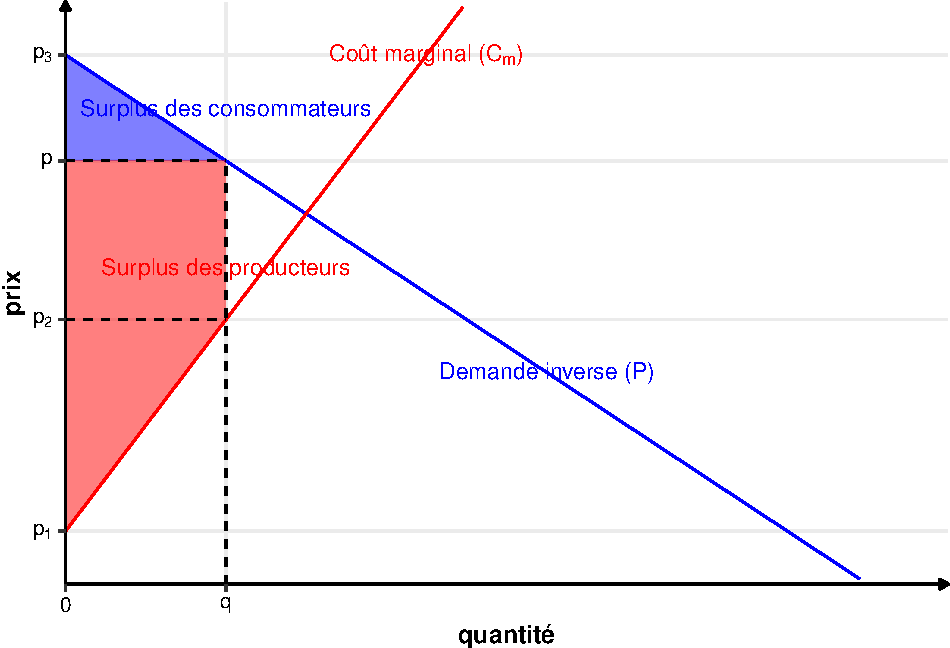
\includegraphics{_main_files/figure-latex/annexesurplus2-1.pdf}
\caption{\label{fig:annexesurplus2}Surplus avec un prix de l'échange \(p\).}
\end{figure}

Le second cas est illustré sur le graphique \ref{fig:annexesurplus3}.
Le prix de l'échange \(p\) est tel que le surplus des consommateurs est un trapèze, et le surplus des producteurs est un triangle.
Dans ce cas, on obtient \(p_2= P(q)\).
Le surplus des consommateurs est donné par :
\[
S_c=\frac{1}{2}\times(p_3-p+p_2-p)\times q
\]
Et le surplus des producteurs par :
\[
S_p=\frac{1}{2}\times(p-p_1)\times q
\]

\begin{figure}
\centering
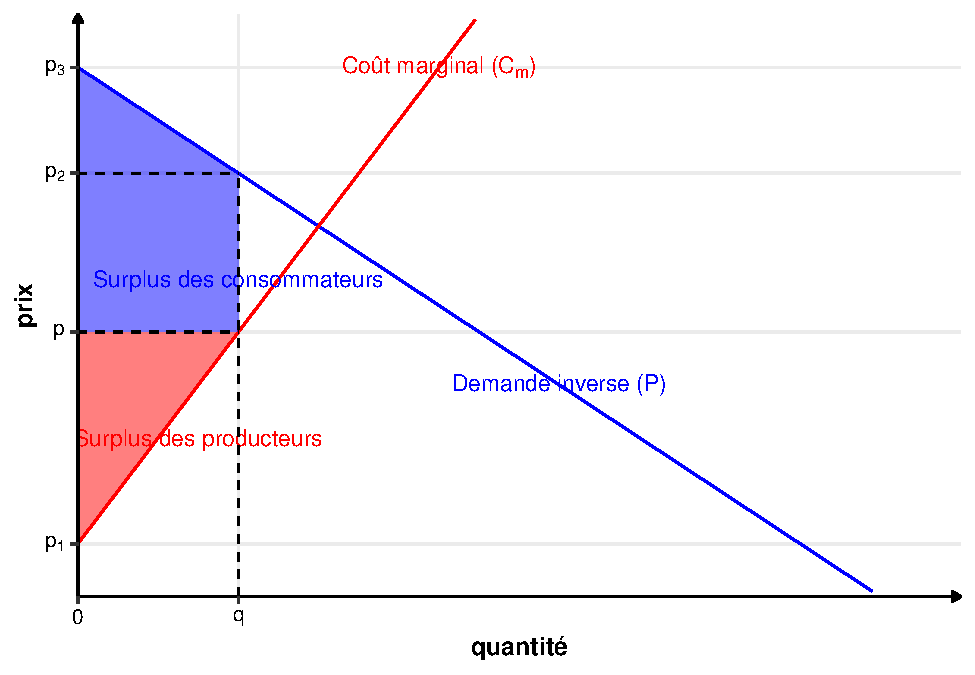
\includegraphics{_main_files/figure-latex/annexesurplus3-1.pdf}
\caption{\label{fig:annexesurplus3}Surplus avec un prix de l'échange \(p\).}
\end{figure}

  \bibliography{book.bib,packages.bib,bibliographie.bib}

\end{document}
